\documentclass[a4paper,12pt]{extarticle} % На предупрежденгие насрать, все норм компиилирутся и славно
% Глобальные поля
\usepackage[left=30mm, top=20mm, right=15mm, bottom=20mm,nohead, includefoot,footskip=35pt]{geometry}

% Язык, кодировка, шрифт
\usepackage[utf8]{inputenc}
\usepackage[T1]{fontenc}
\usepackage[english]{babel}
%\renewcommand{\rmdefault}{Tempora-TLF}
\usepackage{mathptmx}

\usepackage[
    backend=biber,
    style=gost-authoryear,
    movenames=false, % Если авторов больше 4 кеакого-то хрена меняло на название работы
    otherlangs=true
]{biblatex}
\addbibresource{bibliography.bib}
\usepackage{csquotes}

% Межстрочный интервал = 1.5pt
\usepackage{setspace}
\onehalfspacing

% Абзацный отступ = 1.25см
\usepackage{indentfirst}
\setlength\parindent{12.5mm}

% Пакет для содержания
\usepackage{tocloft}

% Команда для специальных разделов (введение, обзор литературы, etc)
% Не нумеруются в содержании, по уровню вложенности:
\newcommand{\specialsection}[1]{
    \phantomsection
    \bigskip\smallskip\hspace{-13.8mm}
    \normalfont\fontsize{12}{12}\textbf{#1}
    \par\bigskip\normalfont\normalsize
    \addcontentsline{toc}{section}{#1}
}

% Размеры заголовков разделов и подразделов
\usepackage{titlesec}
% Раздел: 12pt, добавляем слово "CHAPTER"
\titleformat{\section}
{\fontsize{12}{12}\bfseries}{
\hspace{-1.5mm}CHAPTER \thesection. \hskip-1em}{1em}{}
% Подраздел: 12pt
\titleformat{\subsection}
{\fontsize{12}{12}\bfseries}{\hspace{-0.2mm}\thesubsection}{1em}{}

% Содержание
\renewcommand{\cfttoctitlefont}{\centering\normalsize\bfseries}
\renewcommand{\cftaftertoctitle}{\hfill}

% Слово "Глава" в содержании
\renewcommand{\cftsecpresnum}{CHAPTER\space}
\newlength\mylength
\settowidth\mylength{\cftsecpresnum}
\addtolength\cftsecnumwidth{\mylength}
% Строки с точками
\renewcommand{\cftsecleader}{\cftdotfill{\cftdotsep}}
% Точки после цифр в в содержании
\renewcommand{\cftsecaftersnum}{.}
\renewcommand{\cftsubsecaftersnum}{.}
% Подровнять subsection под точку главы
% (если глав будет больше десяти, будет чуть хуже)
\setlength{\cftsubsecindent}{2.68em}
% Интервал глав
\setlength{\cftbeforesecskip}{4pt}

\renewcommand{\cftsecpagefont}{\normalfont}

% Шрифт подписи (caption) = 12pt
% (Повезло, что small как раз равен 12pt)
\usepackage[font=small,labelfont=bf]{caption}

% Пакет, который позволяет собирать один документ TeX из нескольких
\usepackage{import}

% Пакет, реализующий гиперссылки. Никакого расскрашивания
\usepackage[colorlinks=false,unicode=true]{hyperref}

\newcommand{\ITEM}{\vspace{-0.2cm}\item}
\newcommand{\MList}[1]{\par\begin{itemize}#1\end{itemize}}
\newcommand{\NList}[1]{\par\begin{enumerate}#1\end{enumerate}}


% Задаем отступ у списков равным обычному абзацному отступу (\parindent)
\usepackage{enumitem}
\setlist[itemize]{leftmargin=\dimexpr\parindent\relax}
\setlist[enumerate]{leftmargin=\dimexpr\parindent\relax}

% Нумерация только тех формул, на которые в тексте присутствует ссылка
% \usepackage{autonum}
% Правка нумерации формул: числа справа в скобках
\renewcommand{\theequation}{\arabic{equation}}

% Список литературы
% \makeatletter
% \renewenvironment{thebibliography}[1]
%     {%
%       \bigskip
%       {\noindent\normalfont\bfseries References\par}%
%       \addcontentsline{toc}{section}{References}%
%       \smallskip
%       \list{\@biblabel{\@arabic\c@enumiv}}%
%            {%
%              \settowidth\labelwidth{\@biblabel{#1}}%
%              \leftmargin\labelwidth
%              \advance\leftmargin\labelsep
%              \@openbib@code
%              \usecounter{enumiv}%
%              \let\p@enumiv\@empty
%              \renewcommand\theenumiv{\@arabic\c@enumiv}%
%            }%
%       \sloppy
%       \clubpenalty4000
%       \@clubpenalty \clubpenalty
%       \widowpenalty4000%
%       \sfcode`\.\@m%
%     }%
%     {%
%       \def\@noitemerr
%         {\@latex@warning{Empty `thebibliography' environment}}%
%       \endlist%
%     }
% \makeatother


% Пакеты по желанию (самые распространенные)
% Хитрые мат. символы
\usepackage{euscript}
% Таблицы
\usepackage{multirow}
\usepackage{longtable}
\usepackage{makecell}
% Картинки (можно встявлять даже pdf)
\usepackage[pdftex]{graphicx}

\usepackage{amsthm,amssymb,amsmath}
\usepackage{textcomp}

% Для коректной работы H в фигурах и ссылок на фигуры
\usepackage{float}

\usepackage{hyperref}

\newcommand{\argmax}{\operatornamewithlimits{argmax}}
\newcommand{\argmin}{\operatornamewithlimits{argmin}}
\DeclareMathOperator{\col}{col}
\usepackage{pdfpages}
\begin{document}
    % Оглавление
    %% Титульный лист диплома СПбГУ
% Временное удаление foot на titlepage
\newgeometry{left=30mm, top=20mm, right=15mm, bottom=20mm, nohead, nofoot}
\begin{titlepage}
\begin{center}

\textbf{Saint Petersburg}
\textbf{State University}

\vspace{35mm}

\textbf{\textit{\large Tomin Denis Valerievich}} \\[8mm]
% Название
\textbf{\large Bachelor Diploma Thesis}\\[3mm]
\textbf{\textit{\large Understanding the Aspect Structure of Financial Publications Using Deep Neural Networks}}

\vspace{20mm}
Level of education: Bachelor's degree\\
Direction 01.03.02 “Applied Mathematics and Informatics”\\
Basic educational program CB.5005.2015
«Management»\\
Graduated School of Management\\[25mm]


% Научный руководитель, рецензент
\begin{flushright}
\begin{minipage}[t]{0.65\textwidth}
{Supervisor:} \\
Professor, Research Center for Market Efficiency and Applied Finance, \\ Dr. Darko Vuković

\vspace{10mm}

{Peer reviewer:} \\
Senior Lecturer, Department of Finance and Accounting, \\ Vitaly Leonidovich Okulov
\end{minipage}
\end{flushright}

\vfill

{Saint Petersburg}
\par{\the\year{}}
\end{center}
\end{titlepage}
% Возвращаем настройки geometry обратно (то, что объявлено в преамбуле)
\restoregeometry
% Добавляем 1 к счетчику страниц ПОСЛЕ titlepage, чтобы исключить
% влияние titlepage environment
\addtocounter{page}{1}
    %\pagebreak

    % Заявлениее о самостоятльности
    %\input{}
    %\pagebreak
    
\includepdf[pages=-,             % все страницы файла
            noautoscale=true,    % не менять масштаб
            offset=0mm 0mm,      % поправка позиционирования
            pagecommand={\thispagestyle{empty}}
           ]{struct/start-1.5.pdf}

    % Оглавленине
    \tableofcontents{}
    \pagebreak

    \specialsection{Введение}
    \label{sec:introduction}
    В последние годы наблюдается стремительный рост интереса к применению методов искусственного интеллекта,
в частности машинного (ML) и глубокого обучения (DL), в сфере анализа финансовых данных и принятия
инвестиционных решений. Прогресс в области обработки естественного языка (NLP) и развитие больших языковых
моделей (LLM) позволили значительно расширить спектр решаемых задач, включая анализ новостных публикаций
и прогнозирование цен активов \parencite{Jiang2023, Halder2022, Kim2023}. Тем не менее, несмотря
на достижения в области архитектур и вычислительных возможностей, многие аспекты применения
LLM в финансовом домене до сих пор остаются исследовательски и инженерно нерешёнными.

Современные финансовые рынки характеризуются высокой волатильностью и мгновенной реакцией
на внешние события. Новостные сообщения, изменения регуляторного ландшафта, публикации
финансовых отчётов и рекомендации аналитиков формируют непрерывный информационный поток,
оказывающий как краткосрочное, так и накопительное воздействие на цены активов.
Традиционные аналитические системы, главным образом опирающиеся на количественные
показатели --- такие как цены открытия и закрытия, объёмы торгов и классические технические
индикаторы --- не в состоянии объяснить все ценовые колебания. Вследствие этого их
прогностическая точность снижается, а инвестиционные стратегии становятся уязвимыми
к внезапным рыночным шокам.

Современные финансовые рынки характеризуются высокой волатильностью, непрерывным потоком информации
и мгновенной реакцией на значимые события. Выпуски новостей, изменения регуляторной политики, корпоративные
отчёты и экспертные комментарии могут оказывать как краткосрочное, так и накопительное воздействие на показатели
рынка. Однако традиционные аналитические системы зачастую не способны эффективно интегрировать и интерпретировать
такую разнородную и быстро меняющуюся информацию, что снижает их прогностическую силу и делает инвестиционные
стратегии менее устойчивыми к рыночным шокам.

Решение этих задач требует не только усовершенствования архитектурных решений, но и разработки интерпретируемого,
масштабируемого и воспроизводимого инструментария, способного учитывать контекстуальные особенности финансовых
текстов, извлекать аспекты, релевантные к целевым активам, и обобщать лексико-семантические закономерности.
В настоящей работе предлагается подход, опирающийся на методологическую синергию тематического моделирования,
аспекто-ориентированного анализа и векторных представлений текстов.

Эволюция архитектур NLP-систем привела к доминированию трансформерных моделей, начиная с появления трансформерной
архитектуры в 2017 году \parencite{vaswani2017attention}. Языковые модели на базе BERT \parencite{devlin2019BERT}
и его адаптаций (например, FinBERT \parencite{Liu2020FinBERT,Yang2020FinBERT,Huang2023FinBERT,Araci2019FinBERT})
стали стандартом де-факто в ряде прикладных задач. Однако большинство моделей были обучены на корпусах,
не отражающих специфику финансового языка, что ограничивает их применимость \parencite{Jiang2023, devlin2019BERT}.
Финансовые тексты обладают высокой плотностью терминов, наличием отраслевого жаргона, аббревиатур
и формализованных шаблонов, требующих специализированного подхода к семантическому анализу.

До сих пор открыты вопросы интеграции LLM с классическими количественными моделями, отсутствия
достаточного количества решений с откртым исходным кодом для финансовой области и ограничений
существующих моделей для обработки длинных текстовых последовательностей (см. \hyperref[sec:models]{Раздел 1.3.1}).
В декабре 2024 года была представлена новая современная модель ModernBERT, способная обрабатывать тексты, длина которых
в 16 раз превышает возможности предыдущих архитектур \parencite{Warner2024ModernBERT, devlin2019BERT}. Эта модель
расширяет возможности анализа с отдельного заголовка или поста до целых новостных статей, пресс-релизов, транскриптов
интервью и аналитических обзоров. Несмотря на это, обработка многостраничных финансовых отчётов (например, 10-Q, 10-K)
остаётся сложной задачей (см. \hyperref[sec:limitations]{Раздел 2.1}).

Ранее в подобных исследованиях акцент делался на обработке коротких текстов, таких как заголовки
новостей или постов в социальных сетях, что неизбежно ограничивало доступный контекст и повышало чувствительность
моделей к экспрессивным и стилистически окрашенным элементам текста. Проблема заключается в том,
что такие форматы текстов могут усиливать эффекты эмоционального заголовка или стилистических
приемов, не отражая реального содержания публикации. В настоящей работе данная проблема
нивелируется за счёт анализа полного текста, что позволяет учитывать как эмоциональные,
так и содержательные характеристики новостей, снижая влияние поверхностных факторов.

Таким образом, если рассматривать проблему со стороны управления, при принятии инвестиционных решений на волатильных рынках,
важно своевременно анализировать совокупное влияние различных событий (новости, законодательные изменения, аналитика и т. д.)
на динамику активов. Специалисты не способны справиться с таким объемом информации за предельно короткие сроки. С другой
стороны, отсутствие инструмента для комплексного анализа приводит к запаздывающим или неточным решениям, что снижает
эффективность инвестиционных стратегий и увеличивает риск упущения возможностей.

Разработка инструмента, который мог бы разрешить данную ситуацию и упростить процесс принятия решений является трудоёмкой
и комплексной задачей, которую можно условно разбить на следующие этапы:

\begin{enumerate}
    \item Разработка эффективной архитектуры для LLM.
    \item Адаптация модели под специфику финансового домена.
    \item Тонкая настройка модели для решения конкретных задач.
    \item Интеграция модели в систему, работающую как с количественными, так и с качественными данными,
    включая этапы обучения, тестирования и внедрения.
\end{enumerate}

Важно отметить, что конечной целью подобного инструмента стоит автономное эффективное финансовое прогнозирование, которое
бы могло быть с легкостью интерпретировано финансовым аналитиком, контролирующим систему. Стоит уточнить, что речь
идет об эффективном финансовом прогнозировании именно с точки зрения теории эффективности рынка (EMT) \parencite{emt1970fama}.

Итак, поскольку базовая архитектура ModernBERT уже разработана, а методы прогнозирования стоимости финансовых активов при помощи нейронных
сетей изучены на достаточном уровне, настоящее исследование фокусируется на разработке инструментария для повышения как эффективности, так и
интерпретируемости финансового прогнозирования. Причем исследование формулирует цель достичь повышения эффективности прогнозирования
не за счет количественного или итеративного улучшения имеющихся методов, а за счет изучения принципиально новых областей и качетсвенного
технологического скачка, заключающегося в новой парадигме финансового прогнозирования. Так, настоящее исследование предлагает
достичь качественного скачка за счет расширения модальности данных, использующихся для прогнозирования, а также
разработки методов их предобработки.

Данная задача, как отмечалось ранее, комплексна и крайне трудна. Поэтому предметом работы является не финансовое прогнозирование,
а инструментарий (комплекс методов и конкретные технологии) для интегации языковых моделей, а также методов тематического
моделирования и анализа тональности в процесс прогнозирования стоимости активов, которые сделают возможным в последующих
исследованиях качественный рывок в целевой задаче.

Так, на данный момент, в финансовом прогнозировании LLM используются в крайне узком спектре, так как сама технология относительно нова.
Тем не менее, уже есть первые попытки использовать языковые модели для анализа тональности новостей и интеграции тональностей в процесс
прогнозирования, причем несмотря на ограниченность ресурсов, методов и технологий данный подход зарекомендовал себя как достаточно
эффективный. В частности, модели, применяющие тональности в финансовом прогнозирвании показывают результаты выше тех, что делают
прогнозы, основываясь исключительно на количественных данных \parencite{Kim2023, Jiang2023, Halder2022}. Однако, применимость текстовой
модальности для финансового прогнозирования на данный момент крайне ограничено и новым направлением, пока еще не нашедшем применение
в финансах является аспекто-ориентированый сентиментальный анализ \parencite{SA2020taxonomy,FSA2020problems} и тематическое моделирование
\parencite{angelov2020top2vec,BERTopic2022}.

Таким образом, объектом исследования являются инвестиционные стратегии, основанные на методах искусственного интеллекта. Цель работы
заключается в создании практико-ориентированного интерпретируемого инструментария, на основе которого станет
возможным разработать систему для динамического мультимодального прогнозирования стоимости актива с использованием иерархического
аспекто-ориентированного сентиментального анализа. Отдельно стоит подчеркнуть, что ключевым условием предложенного решения является
его интерпретируемость в отличие от других решений, использующих глубокие нейронные сети как черный ящик.

На протяжении исследования были выполнены следующие работы:

\begin{itemize}
    \item Анализ и выбор современных и наиболее эффективных архитектур и моделей (см. Разделы \hyperref[sec:ml_algos]{1.2} и
    \hyperref[sec:models]{1.3}) для целевой задачи.
    \item Проектирование концепта прицнипиально новой системной архитектуры для эффективного финансового прогнозирования
    (см. Раздел \hyperref[sec:architecture]{3.1}).
    \item Разработка финансовой аспекто-ориентированной гибридной семантической системы (Financial Aspect-Based hybrid Semantic System, FinABYSS),
    направленной на реализацию необходимых системных комонент для интерпретируемой финансовой аналитики на мультимодальных данных
    (см. Раздел \hyperref[sec:components]{3.2}).
    \item Сбор большого и исчерпывающего корпуса финансовых публикаций размером более 15Гб, пригодного для использования в смежных финансовых исследованиях
    (см. Раздел \hyperref[sec:data_governance]{2.2}).
\end{itemize}

Следует подчеркнуть глобальную значимость данного исследования. Несмотря на то что в качестве
предмета экспериментов выбран рынок США, это обусловлено исключительно изобилием, доступностью
и единообразием открытых данных по данному рынку. Методология и инструментарий, разработанные
в работе, легко масштабируются и адаптируются к любым другим финансовым рынкам. Универсальность
подхода гарантирует его применимость в различных юрисдикциях и на различных уровнях развития
информационной инфраструктуры, что подчёркивает принципиальную глобальность исследования.

Все результаты данного исследования, включая код для сбора данных, обучающий код, результаты анализ данных и моделей, а также сами модели доступны
в официальном GitHub репозитории проекта\footnote{FinABYSS (Financial Aspect-Based hybrid Semantic System) [Electronic resource] //
Томин Д.В. --- 2025 --- URL: \url{https://github.com/denisalpino/FinABYSS} (Дата обращения: 26.05.2025). --- Режим доступа: по запросу.}.
Собранный корпус доступен в репозитории HuggingFace\footnote{YahooFinanceNewsRaw [Electronic resource] //
Томин Д.В. --- 2025 --- URL: \url{https://huggingface.co/datasets/denisalpino/YahooFinanceNewsRaw} (Дата обращения: 20.04.2025). --- Режим доступа: по запросу.}.

    % Первая теоретическая глава
    \newpage
    \section{ТЕОРЕТИЧЕСКИЙ ОБЗОР}
    \label{sec:theory}
    \subsection{Artificial Intelligance in Finance}
\subsubsection{Прогнозирование стоимости}
Существует множество подходов, демонстрирующих эффективность прогнозирования стоимости активов с помощью
глубоких нейронных сетей. Наиболее распространёнными в этой задаче являются рекуррентные нейронные сети
(Recurrent Neural Networks, RNN), тогда как сверточные нейронные сети (Convolutional Neural Networks, CNN)
используются преимущественно в качестве вспомогательного компонента.

Наиболее характерным представителем семейства RNN является архитектура долгой кратковременной памяти
(Long Short-Term Memory, LSTM) \parencite{Hochreiter1997LSTM}, часто применяемая для прогнозирования
цен. Её модификации, такие как двунаправленная LSTM (Bidirectional LSTM, Bi-LSTM) и гибридные модели
CNN-LSTM, также показывают высокую результативность. Более того, с появлением трансформерной архитектуры
\parencite{vaswani2017attention} всё активнее исследуются методы её адаптации к специфике временных рядов
\parencite{wen2022transformers}.

В числе последних экспериментов особенно выделяются:

\begin{itemize}
    \item репозиторий, в котором демонстрируется потенциал трансформерной архитектуры на примере прогнозирования
    цены Биткоина\footnote{Bitcoin Price Prediction Using Transformers [Electronic resource] //
    baruch1192. --- 2025 --- URL: \url{https://github.com/baruch1192/-Bitcoin-Price-Prediction-Using-Transformers} (Дата обращения: 11.01.2025).};
    \item исследование, сравнивающее производительность моделей Bi-LSTM, гибридных CNN-Bi-LSTM и трансформера
    при прогнозировании стоимости акций IBM\footnote{CapMarket [Electronic resource] //
    JanSchm. --- 2025 --- URL: \url{https://github.com/JanSchm/CapMarket} (Дата обращения: 18.12.2024).};
    \item торговый робот на базе LSTM, ориентированный на извлечение краткосрочной прибыли в боковом движении
    цены актива CGEN, показавший при бэктестинге доходность в размере 4\% депозита за сутки
    \footnote{Stock Price Prediction with a Bot [Electronic resource] //
    roeeben. --- 2025 --- URL: \url{https://github.com/roeeben/Stock-Price-Prediction-With-a-Bot} (Дата обращения: 27.12.2024).}.
\end{itemize}



Тем не менее отдельные модели, будь то LSTM или методы на основе деревьев решений, обладают ограниченной
адаптивностью при смене рыночных режимов и плохо реагируют на их динамику \parencite{Vukovi2024}.
Несмотря на очевидность этого факта, исследователи нередко недооценивают его значение. Согласно теории
эффективного рынка (Efficient Market Theory, EMT), предложенной Фама в 1970 году, цены активов отражают
всю доступную рыночную информацию, что ставит под сомнение возможность точного прогнозирования на основе
лишь исторических количественных показателей --- цены открытия, закратия, максимума, минимума (Open High
Low Close, OHLC), объёма торгов и классических индикаторов.

К тому же большинство моделей не учитывают такие тонкие аспекты, как заявки лимитного порядка, влияние
других торговых роботов, а также качественную внебиржевую информацию. Новейшие исследования показывают,
что интеграция анализа информационного поля за пределами биржи в прогнозные модели заметно повышает качество
предсказаний, о чём будет подробно рассказано в последующих подразделах.

\subsubsection{Анализ тональности}
Как отмечалось во введении, появление трансформерной архитектуры позволило моделям глубокого обучения
достичь значительного прогресса в понимании естественного языка (Natural Language Understanding, NLU).
Это имеет особую ценность для финансовой сферы, где традиционные количественные данные недостаточны
для точного прогнозирования.

Еще до распространения современных языковых моделей для анализа тональности текста (Sentiment Analysis,
SA) применялись LSTM-модели, ULMfit, авторегрессионные сети и другие методы
\parencite{Hochreiter1997LSTM, howard2018ULMFIT}. Например, в одном исследовании сравнивали
авторегрессионную модель без учета тональности с аналогичной моделью, интегрировавшей
тональностные признаки. Результаты показали, что в 77.8\% случаев модель с учетом тональности
превосходила версию, обученную только на количественных данных \parencite{NNAR2019}.

Современные предобученные трансформерные модели, известные как большие языковые модели (Large Language Model,
LLM), открывают новые возможности для финансового прогнозирования. Наиболее очевидное применение ---
анализ тональности новостей. Для этого требуется сбор значительного объема текстовых данных с последующей
разметкой. Метки классов обычно включают три категории: -1 (негативный), 0 (нейтральный) и 1 (позитивный)
\parencite{SA2020taxonomy}.

Ручная разметка предполагает привлечение отраслевых экспертов, способных оценить влияние текста
на финансовые рынки. Для повышения качества данных применяется метод перекрестного консенсуса \parencite{consensus1997bogdan}:
несколько экспертов независимо аннотируют одни и те же тексты, после чего метки согласуются.
Именно этот подход использовался при создании популярного датасета FinancialPhraseBank \parencite{Malo2014FPB} для тонкой
настройки моделей под задачу финансового анализа тональностей (Financial SA, FSA).

Алгоритмические методы, основанные на динамике стоимости активов, менее распространены из-за
субъективности и нестабильности. В частности по той причине, что сложно определить пороговое
значение изменения цены для классификации тональности и гарантировать, что фактический прирост
не обусловлен любым другим фактором.

После разметки данных, на что уходит большая часть ресурсов, выполняется тонкая настройка
предобученных языковых моделей путем модификации весов на последних слоях нейросети.

Таксономия SA включает три уровня \parencite{SA2020taxonomy}:

\begin{itemize}
    \item \textbf{Документальный уровень.} Тональность оценивается для всего документа (новости, отчета и т.д.).
    Данный уровень предполагает наличие в документе мнений об одной сущности, что редко соответствует реальности.
    Более того, существует и техническое ограничение --- современные трансформеры технически не способны
    обрабатывать многостраничные документы (например, отчеты 10-K) или новостные статьи, вследствие ограниченных
    возможностей обработки токенов. Тем не менее, в последнее время стали появляться модели, способствующие обработки
    хотя бы новостных статей, однако отчеты все еще не могут быть обработаны ими.
    \item \textbf{Уровень предложений.} Тональность относится к одному или нескольким предложениям (обычно 1-8 предложений),
    при этом сохраняется предпосылка об одном субъекте. Именно работы данного уровня преобладают в общем числе благодаря
    доступности датасетов и технической совместимости с современными LLM, из которых практически все способны обработать
    тексты такого размера. Типичные источники --- заголовки новостей, публикации в социальных сетях X (бывший Twitter) и Reddit.
    \item \textbf{Аспектный уровень (Aspect-Based SA, ABSA).} Выявление тональности по отношению к отдельным аспектам сущности.
    ABSA на данный момент является наиболее  продвинутым уровнем, который довольно часто рассматривают как отдельную и достаточно
    обширную область. ABSA включает четыре подзадачи: извлечение аспектов, определение их полярности, категоризация аспектов
    и оценка полярности категорий. Отдельно выделяют таргетированный ABSA, который допускает несколько субъектов, но предполагает
    не более одного сентимента на каждого из них. Более подробно ABSA рассматривается в \hyperref[sec:absa]{Section 1.1.3}.
\end{itemize}

Большинство методов SA требуют разметки текстов, что является существенным недостатком, в ввиду больших ресурсных затрат,
а также имеет естественные ограничения:

\begin{itemize}
    \item Не существует универсального и точного определения тональности, подходящего для каждой задачи. Это вынуждает формулировать
    уникальное определение в ходе решения практических задач, что затруднительно из-за многочисленности паттернов
    и сценариев, встречающихся в текстах.
    \item Невозможно без кратного увеличения затрат на контроль (например, при помощи метода перекрёстного консенсуса
    \parencite{consensus1997bogdan}) обеспечить надежность и объективность оценок, так как на качество разметки
    сильно сказывается человеческий фактор.
\end{itemize}

Как было отмечено, постановка SA может несколько отклоняться от своей классической постановки в контексте различных доменов.
Так, особенностью FSA является то, что он фокусируется не исключительно на обособленных текстах, но так же и на количественной
информации, которая в финансовых статьях крайне много \parencite{FSA2024techniques}.

Тем не менее, FSA терпит неудачи в нескольких типовых сценариях среди которых: нереальные настроения (условные настроения,
сослагательное наклонение, повелительное наклонение), риторика (негативные заявления, персонификация, сарказм), зависимые
мнения, неопределенные аспекты, нераспознанные слова (жаргонизм, микротекст, сущности) и external references (то есть
отсылки к тем знаниям, которые не заключены в модель) \parencite{FSA2020problems}.

\subsubsection{Аспектный анализ}
\label{sec:absa}
ABSA представляет собой специализированную задачу выявления и оценки сентимента по отношению к конкретным
«аспектам» --- характеристикам или свойствам рассматриваемого объекта. В финансовой сфере такими аспектами
могут выступать рисковые факторы, кредитная политика, макроэкономические индикаторы и другие элементы,
упоминаемые в публикациях. Классический подход к ABSA включает три этапа: выделение аспектов из текста,
определение полярности сентимента по каждому аспекту, и агрегацию результатов для построения итоговой
картины мнений экспертов или рынка .

Параллельно с развитием ABSA в лингвистическом сообществе активно развалось тематическое моделирование,
главной целью которого является выявление скрытых «тем» (topics) в корпусах документов. Одним из первых
и наиболее влиятельных методов стал Latent Dirichlet Allocation (LDA) \parencite{LDA2003}, где темы
формулируются как распределения слов, а документы рассматриваются как смеси таких распределений. В контексте
финансовых текстов LDA позволяет выделять основные направления обсуждения (например, «монетарная политика»,
«корпоративные риски» и т.д.), но испытывает сложности с моделированием синтагматических связей и динамичной
лексики.

На стыке эмбеддинговых моделей и тематического анализа сформировалась идея top2vec \parencite{angelov2020top2vec},
согласно которой темы представляются в том же векторном пространстве, что и слова, что позволяет объединить
преимущества распределённых представлений и тематических структур. Далее эволюция привела к появлению BERTopic
\parencite{BERTopic2022}, где для построения тем используются плотностные алгоритмы поверх эмбеддингов, а зате
 для каждого кластера извлекаются наиболее характерные ключевые слова. Эта модель демонстрирует высокую
 адаптивность к изменениям лексики и позволяет работать с динамическими, даже мультиязычными корпусами.

Связь между ABSA и тематическим моделированием очевидна: аспекты в широком смысле являются темами, по отношению
к которым измеряется сентимент. В традиционном ABSA аспекты задаются или извлекаются на основе лингвистических
паттернов (например, правилами на зависимостях или словарями), тогда как тематическое моделирование открывает
путь к автоматическому выявлению аспектов как скрытых латентных переменных. Преимущество такого подхода
в финансовом домене заключается в том, что заранее неизвестное множество аспектов («тем») может быть извлечено
без ручной разметки, после чего к выявленным кластерам документов применяется стандартная процедура оценки
сентимента (например, с помощью LLM), что позволяет получать более полный и интерпретируемый анализ мнений рынка.

Таким образом, в рамках данной работы аспекты рассматриваются как темы в тематическом моделировании. А работа
предлагает способ первоначальной кластеризации векторных представлений, которая формирует «тематические кластеры»,
для того, чтобы агрегировать по ним сентимент. Такое объединение позволяет (1) выявлять как глобальные тренды,
так и локальные, нишевые аспекты финансового рынка, (2) минимизировать необходимость ручной разметки аспектов,
и (3) обеспечить интерпретируемость результатов за счёт явной привязки сентимента к темам, выраженным через
ключевые термины каждого кластера. Это сочетание взяло лучшее от обоих направлений: структуры тем
при LDA/topic2vec/BERTopic и точности полярности при ABSA.

\subsection{Machine Learning Algorithms}
\subsubsection{Dimensionality Reduction}
\textbf{Principal Component Analysis (PCA)} is a linear dimensionality reduction (DR) method based
on the decomposition of the covariance matrix of the original data. Given a zero trait mean,
it finds the covariance eigenvectors (components) responsible for the maximum variance:
$\Sigma = X^T X$, $\Sigma w_i = \lambda_i w_i$, the projection of the data $Y = XW_{d'}$
onto the first $d'$ eigenvectors.

PCA aims to preserve as much variance of the original data as possible and, as a consequence,
preserves well the “global” cluster structure \parencite{TRIMAP2019}. In practice, PCA is often
used as an intermediate step: for example, when dealing with high-dimensional text embeddings
(several hundred features, e.g., embeddings of dimensionality 768) before non-linear
DR methods. The use of PCA can significantly reduce the dimensionality
(down to tens to hundreds of components) and speed up subsequent computations\parencite{huang2022towards}.

However, PCA is a linear method, and it does not capture the more complex nonlinear dependencies
inherent in language embeddings. As a consequence, subtle local word-document relationships
may be lost, although the overall structure (the “global landscape” of the data) is most often
preserved.

\textbf{t-distribution Stochastic Meighbor Embedding (t-SNE)} is a nonlinear stochastic method focused
on preserving local data structure. In high-dimensional space, it computes conditional probabilities
$p_{j|i} \propto \exp(-|x_i-x_j|^2/2\sigma_i^2)$, reflecting the proximity of neighbors; it then
symmetrizes them: $p_{ij}=(p_{j|i}+p_{i|j})/2n$. A similar measure (Student's distribution with 1 degree
of freedom) is given in the low-dimensional mapping. The algorithm optimizes the placement of $Y$ points
by minimizing the Kullback-Leibler divergence $C = \sum_{i,j} p_{ij}\ln\frac{p_{ij}}{q_{ij}}$.
As a result, points close to each other in the original space will retain a local cluster structure
in the low-dimensional space.

The 'perplexity' hyperparameter determines the number of effective neighbors. t-SNE shows an impressive
visualization of local clusters, but poorly reproduces the global distance between clusters.
It is computationally expensive for large samples and is usually used only for the final transition
to 2D space (or 3D), not for intermediate DR. For textual embeddings, t-SNE is
often applied after preprocessing (e.g., PCA mapping) because it scales poorly directly
to several hundred features.

\textbf{Uniform Manifold Approximation and Projection (UMAP)} is a method of nonlinear DR
based on the manifold assumption. UMAP theoretically relies on Riemannian geometry and the theory
of “fuzzy simplicial sets”. The algorithm constructs a graph of $k$-nearest neighbors
in the original space, then each pair of points is assigned a “membership” in a fuzzy set by a formula of the form:

\begin{equation}
    \mu_{ij}=\exp\big(-\cfrac{\max(0, d(x_i, x_j) - \rho_i)}{\sigma_i}\big),
\end{equation}

where $\rho_i$ takes into account the density of neighbors. These local symplectic sets are then combined
and symmetrized, and a weighted data graph is obtained. Next, a similar “fuzzy” graph is constructed in
low-dimensional space and the location of points is optimized by minimizing the cross entropy energy between
the two graphs.

UMAP retains the local structure of the data while aiming to distribute points uniformly on the manifold;
unlike t-SNE, it can better retain some global features (due to the cross-entropy used). The main hyperparameters
of UMAP are the number of neighbors 'n\_neighbors' (specifies the scale of locality) and 'min\_dist'
(minimum distance of points in the mapping).

UMAP demonstrates high speed and scalability (the method can run on an arbitrary number of output measurements
at once). In an experiment, UMAP was shown to give a visualization quality comparable or better than t-SNE
with a significantly shorter runtime \parencite{UMAP2018mcinnes}. UMAP's advantages also include the preservation
of a larger-scale data structure and the ability to “downscale” the dimensionality down to multidimensional
vectors (not only 2D).

Nevertheless, UMAP may incorrectly represent highly sparse clusters by “equalizing” dense and sparse regions
(the algorithm actually seeks a uniform distribution of data on the assumed manifold). In addition, UMAP
results are sensitive to the choice of hyperparameters and the degree of noise sampling (the algorithm uses
approximate neighbor search and negative sample sampling) \parencite{huang2022towards}. However, in most textual
data clustering applications, UMAP has proven to be a robust and efficient tool.

There are several Python implementations of this method. The classical implementation, 'umap-learn' (CPU),
is widely used \parencite{mcinnes2018umap-software}, and there is a GPU implementation ('cuML') to speed
up the learning process \parencite{cuml2020machine}. cuML's GPU implementation of UMAP can give speedups
of up to 10-100× compared to the CPU version on large amounts of data. However, in early versions of cuML,
approximations were introduced for speed purposes, sometimes resulting in a small difference in display
quality compared to the original. Also the GPU implementation of UMAP may reduce the local structure preservation
relative to the reference version. Thus, 'cuML' UMAP is suitable for very large amounts of data, while
the implementation from 'umap-learn' is more versatile and stable, but runs slower.

\textbf{Triplet Manifold Approximation and Projection (TriMAP)} is an embedding learning method with an emphasis
on the global \parencite{TRIMAP2019} data structure. It formulates the problem through triples of $(i,j,k)$
points: point $i$ must be closer to $j$ than to $k$ in a low-dimensional representation. The selection
of such triplets is based on nearest and farthest neighbors in the original space; each triplet is given
a weight reflecting the relative closeness of the pairs in the original space. Optimization is performed over
a large sample of informative triplets using gradient descent.

TriMAP preserves global structure much better than t-SNE and often better than UMAP. TriMAP also scales well
and exhibits low runtime for large and high-dimensional samples \parencite{TRIMAP2019}. In terms of text embeddings,
TriMAP can provide a more readable picture of document cluster locations on 2D (although local community details
may be smoothed out).

\textbf{Pairwise Controlled Manifold Approximation and Projection (PaCMAP)} is a newer method specifically designed
to balance local and global structure \parencite{PACMAP2021}. Like TriMAP, it uses samples of pairs of points
of different types: “close” pairs (neighbors), "middle" pairs (between clusters), and "far" pairs. For each
pair type, the corresponding weights and attraction/repulsion forces are specified. As a result, the optimized
loss function tends to simultaneously compress locally close points and push distant ones apart, preserving
the global shape of the distribution.

PaCMAP is robust to hyperparameter selection and DR in preprocessing, and preserves both
local and global structure well. The disadvantages of PaCMAP are its relative novelty and the need to fit
fractions of different types of pairs.

Systematic comparisons indicate a characteristic separation in the properties of these algorithms. Thus, PCA,
TriMAP, and PaCMAP preserve global distances (large-scale cluster structure) well, while t-SNE and UMAP are better
at capturing local details \parencite{huang2022towards}. PCA is traditionally used for preprocessing: reducing
the dimensionality to tens of components speeds up further analysis and makes it more stable. However, it is
noticeable that full PCA preprocessing can distort the original distances, so the results of the final embedding
(e.g., t-SNE/UMAP visualization) often depend on the number of PCA components. In experimental method evaluations,
PaCMAP and TriMAP showed the best agreement of global distances, while UMAP and t-SNE were on average inferior
in this task. Conversely, t-SNE and UMAP performed best in the classification task on vector features (testing
local consistency).

In general, the choice of DR method for high-dimensional embeddings of documents depends
on the task: for subsequent clustering and thematic one often uses PCA or UMAP (for more “stable” representation
of clusters), and for final 2D visualization and detailed analysis of local clusters --- t-SNE, UMAP or PaCMAP.
Careful selection of hyperparameters and possibly a combination of methods (e.g., PCA+UMAP) can achieve a better
representation of the textual data structure.

\subsubsection{Clustrering}
In the considered scheme for thematic analysis of financial news articles, a DR
algorithm is applied after obtaining textual embeddings. After this DR,
clustering algorithms operate in a less sparse space, which can improve
the selection of dense regions and reduce the influence of noise factors.

\textbf{K-Means} is one of the classical partitional clustering algorithms \parencite{kmeans2010data}.
It seeks to partition the data into $K$ clusters by minimizing the intra-cluster point spread.
We denote clusters $C_1,\dots,C_K$ and cluster centroids $\mu_k$; then the optimized objective
function (the “sum of squares of distances” metric from points to the corresponding centroids)
is given as

\begin{equation}
    J(C)= \sum_{k=1}^K \sum_{x_i \in C_k} \|x_i - \mu_k\|^2,
\end{equation}

and is minimized when partitioned by the Euclidean metric. Finding the global minimum of this
function is an NP-complete problem, so the K-Means method performs a greedy iterative procedure
of point reclassification and centroid recalculation (usually with random initialization) that
converges to a local minimum. An important feature of K-Means is the requirement to specify
the number of clusters $K$ and the initial approximations in advance.

Since the algorithm typically uses a Euclidean metric, it forms mostly spherical clusters. All
objects are automatically assigned to some cluster (rigidly “belonging” each point to one cluster),
and the algorithm does not explicitly emphasize outliers or noise. Advantages of the method include
ease of implementation, low computational cost, and widespread use. However, K-Means is unstable
to outliers, and is poor at distinguishing nested or highly heterogeneous clusters.

\textbf{Density-Based Spatial Clustering of Applications with Noise (DBSCAN)} is a density-based
clustering method \parencite{DBSCAN1996}. It defines clusters as regions of high-density data separated
by low-density regions. The algorithm uses two parameters: the radius $\epsilon$ and the minimum
number of points $min_{pts}$. A point is called the “core” of a cluster if its $\epsilon$-neighborhood
contains at least $min_{pts}$ points. Points reachable in density from the core belong to the same
cluster.

DBSCAN automatically separates points that are not in dense regions as noise and does not require
the number of clusters to be specified. Due to this, the method finds clusters of arbitrary shape
and is well suited for datasets with non-uniformly distributed objects. However, DBSCAN has significant
limitations: the choice of a single $\epsilon$ threshold is critical, and when combining clusters
of different densities, the algorithm either merges them into one whole or breaks them into too small
fragments. In addition, as the dimensionality of the space grows, the data becomes sparse, and it becomes
difficult to distinguish a high-density region from a low-density one. As a consequence, DBSCAN
in high-dimensional text embeddings often demonstrates reduced efficiency. Also, the complexity
of classical DBSCAN in the absence of optimization can reach $O(n^2)$, although practical implementations
with indexes usually have significantly lower performance.

\textbf{Hierarchical DBSCAN (HDBSCAN)} is a hierarchical extension of the DBSCAN method \parencite{HDBSCAN2013}.
Unlike DBSCAN, HDBSCAN does not require a fixed $\epsilon$: instead, it computes the mutual reachability
distance between points $x$ and $y$ as

\begin{equation}
    d_{\mathrm{mreach}}(x,y) = \max\bigl\{d_{\mathrm{core}}(x),\,d_{\mathrm{core}}(y),\,d(x,y)\bigr\},
\end{equation}

where $d_{\mathrm{core}}(x)$ is the distance from a point $x$ to its $k$-th nearest neighbor (i.e.,
the minimum $\epsilon$ at which $x$ becomes the “core” of the cluster). We then construct a graph
of complete mutual reachability (or directly a minimal island tree at such distances). By removing
the edges of this tree in descending order of weight, the algorithm generates a tree-like hierarchy
of clusters reflecting the nested structure of the data at different density thresholds. From this tree,
the final clusters are selected based on the stability criterion. Such a procedure is equivalent
to performing multiple runs of DBSCAN at all possible $\epsilon$ and selecting the most significant
“stable” clusters. An important feature of HDBSCAN is that it finds the optimal number of clusters
by itself, requiring only a minimum cluster size ('min\_cluster\_size').

Thanks to its hierarchical approach, HDBSCAN is able to detect nested clusters of different densities
and adapt more flexibly to the data distribution than DBSCAN and K-Means. The algorithm is robust
to density fluctuations: if there are regions of different homogeneity in the data, HDBSCAN will identify
large sparse clusters and smaller dense clusters simultaneously. It automatically flags outliers, similar
to DBSCAN, but without rigidly binding to a single threshold. Because of the additional processing
(searching for $k$-nearest neighbors, MST construction, and hierarchy analysis), HDBSCAN is somewhat
more computationally complex, but modern implementations with efficient neighborhood structures usually
provide comparable or even better performance \parencite{HDBSCAN2017software}. In general, HDBSCAN
provides a richer description of the data structure at different levels of granularity and more often
yields more meaningful clusters in complex multidimensional spaces.

Existing experimental studies show that in the task of topic analysis of long texts, each method has its
own pros and cons. K-Means is often used as a basic method due to its simplicity and scalability, but
it gives a relatively coarse partitioning of topics because it is limited by the spherical shape
of clusters and requires the number of topics to be specified in advance. DBSCAN can detect arbitrarily
shaped clusters and separate noise, but its performance is reduced on high-dimensional embeddings of texts
due to sparsity and the need to tune the global density threshold.

In many comparative experiments, HDBSCAN is shown to outperform both mentioned methods in terms
of the quality of topic clusters: it automatically adapts to the variability of embedding density, detects
nested topics of different granularity, and reliably eliminates irrelevant noise
\parencite{HDBSCAN2017software, HDBSCAN2013}. These findings are supported by practical applications
(e.g., news article clustering), where HDBSCAN most often yields more interpretable and stable results
compared to K-Means or “flat” DBSCAN \parencite{BERTopic2022}.

\subsubsection{Evaluation}
In the joint optimization problems of DR and clustering algorithms, it is critical
to apply metrics that can simultaneously evaluate the quality of the projection and the purity of the selected
groups. The two most common metrics in this context are the silhouette index \parencite{silouette1987}
and the DBCV index \parencite{dbcv2014density}.

The silhouette coefficient characterizes, for each object, the ratio of the average intra-cluster distance
to the nearest extra-cluster distance \parencite{silouette1987}. For object $i$ the following are calculated

\begin{equation}
    a(i)=\frac{1}{|C_i|-1}\sum_{j\in C_i\setminus\{i\}}d(i,j),\quad b(i)=\min_{C\neq C_i}\frac{1}{|C|}\sum_{j\in C}d(i,j),
\end{equation}

where $C_i$ is the cluster containing $i$, and $d(\cdot,\cdot)$ is the metric (usually Euclidean). Then

\begin{equation}
    s(i)=\frac{b(i)-a(i)}{\max\{a(i),\,b(i)\}}\in[-1,1].
\end{equation}

The mean $s=\frac1N\sum_i s(i)$ reflects how compact and distant objects within clusters are from neighboring
clusters.

The silhouette coefficient is well suited for assessing separability for “spherical” clusters, but
for density-based separability (different cluster densities and shapes) it can give overestimates or distorted
estimates, since in this case intra-cluster and inter-cluster distances do not reflect the quality of density
regions. In particular, the same is true for other indices of similar metrics, such as the Davis-Bolden and
Calinski-Harabasz index \parencite{mmj2023liu}. All of them rely on average distances to centers or variance across clusters
and do not take into account density heterogeneity and noise extraction \parencite{liu2024newindexclusteringevaluation}.

Thus, was developed a density-based metric specifically for DBSCAN/HDBSCAN clustering, the Density-Based Clustering Validation
Index (DBCV) \parencite{dbcv2014density}. This metric measures the average density ratio of “within - between” clusters,
and also explicitly handles noise and arbitrary cluster shape. Together, it allows correct estimation of arbitrarily shaped
clusters, which strictly speaking are called irregular clusters.

On the other hand, DBCV has a key disadvantage --- when clusters overlap, it gives a higher score to their union than to their
dissection, which can negatively affect exactly hierarchical density clustering. Another problem with existing cluster
validity indices is the assumption that data within a cluster has a uniform distribution, even if the shape of the cluster
is arbitrary.

There are also other metrics, such as VIASCKDE \parencite{viasckde2022} and Min-Max-Jump Silhouette coefficient (MMJ-SC)
\parencite{mmj2023liu, liu2024newindexclusteringevaluation}, they clearly have potential in a fairly wide range of tasks,
but are still inferior to DBCV in stability on a different tasks and test cases \parencite{liu2024newindexclusteringevaluation}.
Moreover, as example, MMJ-SC is absolutely new metric that have not been tested enough yet.

On the test data of clusters of complex nested shapes in three-dimensional space, the DBCV index is the only metric that
performed correctly, showing a maximum value of 0.53 on the true clustering variant, while the silhouette coefficient,
although it showed a higher maximum value of 0.62, but this maximum of the metric came from the categorically incorrect
cluster partitioning \parencite{liu2024newindexclusteringevaluation}.

\subsection{Deep Neural Networks}
\subsubsection{Модели}
Изначально в аналитике финансовых текстов применялись классические рекуррентные \parencite{RNN1986} и сверточные \parencite{CNN1998lecun} сети.
Рекуррентные сети, включая улучшенные варианты LSTM \parencite{Hochreiter1997LSTM}, способны обрабатывать текст как последовательность,
моделируя контекст слова на основе предыдущих состояний. Поворотным этапом стал переход к трансформерам \parencite{vaswani2017attention}.


\textbf{Представления двунаправленного кодировщика трансформера (Bidirectional Transformer Encoder Representations,
BERT)}. Модель BERT \parencite{devlin2019BERT} предложила двунаправленный кодировщик на основе механизмов внимания,
что позволило учитывать контекст слова одновременно слева и справа. BERT задаёт новую парадигму: модель предобучается
на больших корпусах на задаче моделирования маскированного языка (Masked Language Modeling, MLM), а затем тонко
настраивается под конкретные задачи.

Ключевой архитектурной особенностью BERT является полносвязная модель трансформера с механизмом Multi-Head Attention
и скрытыми слоями Feed-Forward (в BERT-base – 12 слоёв по 768 нейронов). При этом BERT базово ограничен длиной входной
последовательности (до 512 токенов), что ставит ограничения на обработку длинных документов. Зато архитектура BERT
оказалась крайне удачной для тонкой настройки: она хорошо зарекомендовала себя в классификации, вопросно-ответных
системах и других задачах при минимальных изменениях слоёв вывода.



\textbf{Финансовый BERT (FinBERT)}. Для финансового домена были разработаны адаптированные версии BERT --- FinBERT.
Так, в 2019 году была разработана модель FinBERTv1 \parencite{Araci2019FinBERT}, дообученный BERT на финансовом датасете для задачи
анализа тональности. Его модель показала улучшение всех метрик. FinBERTv1 использует стандартную архитектуру BERT,
но имеет специфический словарь финансовых текстов — например, термины из отчетов и новостей. Несмотря на размер
обучающей выборки меньший, чем у моделей общего назначения, Успех FinBERTv1 прежде всего обусловлен тем, что
модель «понимает» контекст финансовой терминологии лучше, чем модели общего назначения.

Позже была разработана другая версия FinBERTv2, специально предобучая её на финансовых корпусах (новости,
отчёты компаний, финансовые форумы) и используя мультизадачное обучение \parencite{Liu2020FinBERT}. Это
позволило FinBERTv2 выучить богатые представления, учитывающие специфику финансовой лексики. FinBERTv2
демонстрирует заметно лучшие результаты на задачах финансового сентимента и вопросно-ответных системах.

Еще одна работа — FinBERTv3 \parencite{Yang2020FinBERT, Huang2023FinBERT} --- также адаптировала BERT
под финансы, но с акцентом на интерпретируемость и извлечение информации из аналитических отчётов. Авторы
развивают идею учета контекста: их FinBERTv1 «интегрирует финансовые знания» и лучше «резюмирует
контекстуальную информацию в финансовых текстах». При этом модель значительно превосходит как словарные
подходы, так и классические алгоритмы машинного обучения, а также свёрточные и LSTM-модели на задачах
классификации тональности в экспериментах с разметкой аналитиков. Особенно сильным преимуществом FinBERTv3 \parencite{Yang2020FinBERT}
является обработка предложений, где другие модели ошибочно ставят метку «нейтрально» --- благодаря лучшему
учёту контекста модель выявляет позитивные/негативные оттенки там, где неглубокие методы промахиваются.

Таким образом, все три варианта FinBERT основаны на архитектуре трансформера BERT, но различаются стратегией
обучения: модель FinBERTv1 просто тонко настроена на специализированном датасете, FinBERTv2 --- предобучена
смешанных данных и задачах, а FinBERTv3 --- упор сделан на извлечение финансовой информации, контекстный
анализ и интерпретацию. Во всех случаях финансовая специализация даёт превосходство над «чистой» моделью
BERT в финансовом домене.

\textbf{ModernBERT} \parencite{Warner2024ModernBERT} --- это новейшее поколение моделей, кодировщиков, эта архитектура сохраняет идею BERT,
но включает несколько усовершенствований. Во-первых, ModernBERT обучен на очень большом объёме данных ($\approx$3
триллиона токенов) и изначально поддерживает длину последовательности до 8192 токенов, в то время как исходный
BERT ограничен 512 токенами. Это качественно меняет способности модели — она может захватывать длинный контекст
документа целиком без специальной пост-обработки. Во-вторых, архитектура ModernBERT включает технологические
новшества: так, в ней применены гейтированные слои GeGLU, использованы ротационные позиционные кодировки (RoPE)
для лучшего кодирования положения на больших расстояниях, а также внедрён чередующийся механизм локально-глобального
внимания вместо полного механизма внимания у BERT. Это позволяет эффективнее обрабатывать длинные тексты с точки
зрения вычислительных ресурсов. Кроме того, ModernBERT оптимизирован для скорости и памяти: он спроектирован
с учётом аппаратных особенностей GPU.

По сравнению с BERT и его «каноническими» модификациями, ModernBERT достигает новых рекордов эффективности. Так,
эта модель превосходит BERT на всех стандартных задачах бенчмарка GLUE (см. Раздел \ref{sec:benchmarks}) и значительно
улучшает показатели в задачах извлечения и поиска по длинным контекстам. Её показатели значительно выше конкурентов
в задачах с длинным контекстом. Например, при построении индексов ColBERT ModernBERT имеет метрику 80.2, в то время,
как для BERT она составляет всего 28.1, а для предыдущей модели с аналогичным контекстом --- 69.3. При этом ModernBERT
также обрабатывает короткий контекст быстрее предыдущих лидирующих моделей, сохраняя при этом экономию памяти
\parencite{Warner2024ModernBERT, devlin2019BERT}. Иными словами, ModernBERT представляет собой «новое поколение»
кодировщиков. Он не только эффективен, но и специально заточен под длинные тексты и большие масштабы данных.

Таким образом, ModernBERT — это эволюционная ступень архитектуры кодировщика. Он сохраняет концепцию двунаправленного
трансформера BERT, но адаптирует её к масштабным данным и длинным последовательностям. Благодаря сочетанию новых
архитектурных приёмов и гигантского корпуса обучения ModernBERT значительно расширяет возможности по обработке финансовых
(и любых других) текстов большого объёма по сравнению с оригинальным BERT.

\subsubsection{Техники}
\textbf{Тонкая настройка.} В современных NLP-системах, основанных на трансформерах, предобученная модель служит
обобщённым языковым ядром, однако она не всегда готова давать оптимальные представления эмбеддингов для конкретных
задач. Тонкая настройка представляет собой дополнительную фазу обучения, в ходе которой уже предобученная модель
корректирует свои внутренние веса под узконаправленные цели. Тонкая настройка задействует размеченные данные
именно для целевой задачи (классификация, регрессия и т. д.). В финансовом тематическом анализе тонкая настройка
критична для того, чтобы модель не просто генерировала универсальные представления текста, а акцентировала внимание
на релевантных паттернах, интенсивности финансовых терминов, синтаксических конструкциях и даже количественных
упоминаниях, что обеспечивает большую точность кластеризации и прогнозных модулей.

Одной из наиболее востребованных downstream-задач является оценка семантичесой схожести текстов (Semantic Textual
Similarity, STS) --- определение смыслового сходства двух текстовых фрагментов. В отличие от бинарных задач классификации,
STS формулируется как задача регрессии: модели требуется выдать непрерывную оценку близости, обычно в диапазоне
от 0 до 5 \parencite{Cer2017STSB} или от 0 до 1 \parencite{gao2021simcse}.

STS-задача предъявляет высокие требования к качеству эмбеддингов: они должны сохранять тонкие семантические нюансы
и одновременно быть инвариантны к синтаксическим перестановкам и стилевым вариациям. Так, была предложена архитектура
Sentence-BERT, где два экземпляра BERT-сети обмениваются градиентами через сиамскую конфигурацию, а их выходные векторы
сравниваются по косинусному расстоянию, что позволило значительно ускорить и улучшить оценку STS \parencite{SBERT2019}.

Таким образом, тонкая настройка эмбеддинговой модели на STS играет ключевую роль в построении пайплайна, где комбинируются
модели понижения размерности и кластеризации. Тонкая настройка обеспечивает эмбеддинги, в которых локальные и глобальные
семантические связи выстроены таким образом, чтобы и нелинейное понижение размерности сохраняло релевантные соседства,
и плотностная кластеризация автоматически выделяла тематические объединения без избыточного шума.

\textbf{Доменно-адаптированное предобучения (Domain-Adaptive Pretraining, DAPT).} В современной практике работы с
LLM оказывается недостаточным одноразовое предобучение на обширных общекорпусных данных. DAPT представляет собой
дополнительную фазу предобучения на текстах целевого домена, предшествующую этапу тонкой настройки на определенной
задаче \parencite{gururangan2020DAPT}.

В отличие от классической тонкой настройки, при которой модель лишь корректирует веса в последних слоях под конкретный
датасет и задачу, DAPT продлевает исходную задачу языкового моделирования, позволяя модели «освежить» и углубить своё
представление о лексике, синтаксисе и семантике специфического домена --- например, финансовых публикаций. Такое поэтапное
наращивание преобучения демонстрирует существенные приросты качества на доменных задачах как в условиях дефицита
размеченных данных, так и при их изобилии.

Исходя из расчетов, DAPT в среднем обеспечивает прирост бенчмарков на 4\% в относительной шкале по сравнению с базовой
моделью, которая не была адаптирована под определенный домен. Данная цифра является весьма весомой, учитывая, что
для некоторых специфичных задач прирост может составлять вплоть до 20\% \parencite{gururangan2020DAPT}.

Необходимость доменной адаптации особенно очевидна в финансовом секторе: общие корпуса, такие как BookCorpus \parencite{BookCorpus2015}
или Wikipedia \parencite{WikiText2017}, не отражают терминологию, метафоры и стилистические паттерны пресс-релизов, аналитических отчётов
и биржевых новостей. Множество исследований подтвердило преимущества DAPT в специализированных областях. Так,
разработчики SciBERT продемонстрировали, что предобучение BERT на корпусе научных статей приводит к улучшению
показателей на задачах извлечения научных сущностей и классификации статей по дисциплинам, обеспечивая рост
F1-метрики до 2-3 пунктов по сравнению с базовой моделью \parencite{SciBERT2019}. Аналогично BioBERT, адаптированный
к биомедицинскому тексту, повысил точность извлечения медицинских терминов и отношений на 10-20\% по сравнению
с исходным BERT \parencite{BioBERT2020}.

В финансовом домене доменная адаптация позволяет LLM лучше улавливать нюансы упоминаний акций, процентных ставок
и регуляторных терминов, что вкупе с задачей тематической кластеризации повышает качество эмбеддингов и делает
выходные представления более «разборчивыми» при последующей кластеризации методом HDBSCAN. Таким образом, DAPT
выполняет роль «моста» между общими языковыми знаниями и потребностями предметной области, позволяя добиться
значительного улучшения результатов на доменных задачах.

\textbf{Механизм слияния.} В многомодальных и многокомпонентных системах механизм слияния отвечает за объединение
информации из разных источников или представлений, обеспечивая совместную обработку гетерогенных сигналов.

Первый --- раннее слияние --- предполагает подачу всех признаков (биржевых котировок, технических индикаторов
и текстовых эмбеддингов) сразу в единую модель CNN‑LSTM \parencite{Karpathy_2014_CVPR, dutt2022shared}. Преимущество
метода --- простота реализации и возможность немедленно учить кросс‑модальные зависимости. Однако на практике
раннее слияние подвержен «захлёбыванию» в шуме одной из модальностей и утрачивает гибкость при динамической
оценке вклада каждой из них \parencite{dutt2022shared}.

Второй метод --- позднее слияние --- объединяет предсказания отдельных каналов (каждая модальность обрабатывается
своей CNN-LSTM-ветвью) лишь на завершающем этапе \parencite{Karpathy_2014_CVPR, ortega2019multimodal}.
Такой подход отличается модульностью (простота замены или дообучения отдельного канала), но исключает
извлечение низкоуровневых кросс‑модальных закономерностей и требует обучения всех ветвей по‑отдельности,
что влечет кратное увеличение вычислительных ресурсов \parencite{dutt2022shared}.

Третий, компромиссный механизм --- медленное слияние --- обеспечивает поэтапное слияние каналов
на разных уровнях сети \parencite{feichtenhofer2016convolutional, dutt2022shared}. Ключевые преимущества метода:
баланс между автономной переработкой каждой модальности и возможностью учёта их взаимодействия, сохранение
«чистоты» низкоуровневых признаков и гибкость настройки числа и глубины этапов интеграции \parencite{Karpathy_2014_CVPR}.
Главные недостатки --- сложность выбора оптимального уровня слияния и повышенные вычислительные затраты из‑за
параллельных ветвей на ранних слоях, но тем не менее, меньшие нежели при позднем слиянии.

\subsubsection{Бенчмарки}
\label{sec:benchmarks}
Бенчмарк общего пониания языка (General Language Understanding Evaluation, GLUE) представляет собой набор из девяти
разнообразных задач на понимание естественного языка, предназначенных для оценки и сравнения производительности моделей
в различных задачах обработки естественного языка (Natural Language Processing, NLP) \parencite{wang2018GLUE}.
Предоставляя стандартизированную основу, GLUE облегчает разработку моделей, которые хорошо обобщаются при решении
различных задач, способствуя прогрессу в создании надежных и универсальных систем понимания языка.

Бенчмарк GLUE представляет собой набор ресурсов для обучения, оценки и анализа систем понимания естественного языка.
GLUE состоит из:

\begin{itemize}
    \item \textbf{Набор из девяти задач}, на понимание языка по предложениям или парам предложений, созданный на основе
    существующих наборов данных и отобранный таким образом, чтобы охватить разнообразный диапазон размеров наборов
    данных, жанров текстов и степеней сложности.
    \item \textbf{Диагностический набор данных}, предназначенный для оценки и анализа работы моделей в отношении
    широкого спектра лингвистических явлений, встречающихся в естественном языке;
    \item \textbf{Публичная таблица лидеров} для отслеживания результатов выполнения эталона и приборная панель
    для визуализации работы моделей на диагностическом наборе.
\end{itemize}

Ниже представлена таблица, иллюстрирующая ключевые характеристики датасетов, используемых в GLUE:

\begin{table}[ht]
    \caption{Обзор датасетов, входящих в бенчмарк GLUE.}
    \centering
    \resizebox{\textwidth}{!}{%
    \begin{tabular}{|l|l|l|c|c|}
        \hline
        \textbf{Название} & \textbf{Задача} & \textbf{Источник} & \textbf{Размер} & \textbf{Метрика} \\
        \hline
        \textbf{CoLA}   & Классификация по одному предложению & \parencite{dudy2018CoLA} & $\sim$8\,500 & Коэффициент корреляции Мэттьюса \\
        \textbf{SST-2}  & Бинарная классификация по одному предложению  & \parencite{socher2013SST2} & $\sim$67\,000 & Точночть \\
        \textbf{MRPC}   & Идентификация перефразирования & \parencite{dolan2005MRPC} & $\sim$3\,700 & Точность, F1 \\
        \textbf{STS-B}  & Семантическое текстовое сходство (Регрессия) & \parencite{Cer2017STSB} & $\sim$7\,000 & Корреляция Пирсона/Спирмена \\
        \textbf{QQP}    & Обнаружение повторяющихся вопросов (пары вопросов Quora) & \parencite{chen2018QQP} & $\sim$364\,000 & Точность, F1 \\
        \textbf{MNLI}   & Многожанровый вывод на естественном языке & \parencite{williams2018MNLI} & $\sim$393\,000 & Точность \\
        \textbf{QNLI}   & Задача вывода & \parencite{rajpurkar2016QNLI} & $\sim$105\,000 & Точность \\
        \textbf{RTE}    & Распознавание текстовых фрагментов & \parencite{bentivogli2009RTE} & $\sim$2,500 & Точность \\
        \textbf{WNLI}   & Задача вывода & \parencite{levesque2012WNLI} & 634 & Точность \\
        \hline
    \end{tabular}
    }%
    \label{tab:GLUE}
\end{table}

В целом, бенчмарк GLUE представляет собой надежную основу для оценки как стандартных, так и адаптированных к конкретной области моделей NLP.
Его комплексный дизайн и включение различных лингвистических задач позволяют провести тонкий анализ возможностей модели.
После этого обзора будет рассмотрен эталон FLUE, предназначенный для оценки моделей в финансовом контексте,
будет рассмотрен для дальнейшего дополнения оценки доменно-адаптивных стратегий предварительного обучения.

Бенчмарк Financial Language Understanding Evaluation (FLUE) представляет собой аналог бенчмарка GLUE, но специализированный
под домен финансов \parencite{FLANG2022FLUE}. Данный бенчмарк был создан совсем недавно на основе 5 разнообразных датасетов.
Его разработка обусловлена необходимостью оценки моделей, способных эффективно обрабатывать финансовый текст, поскольку
стандартные универсальные наборы данных зачастую не отражают специфические особенности финансовой лексики и задач,
присущих данной области.

\begin{table}[ht]
    \caption{Обзор датасетов, входящий в бенчмарк FLUE.}
    \centering
    \resizebox{\textwidth}{!}{%
    \begin{tabular}{|l|l|l|c|c|l|}
        \hline
        \textbf{Название} & \textbf{Задача} & \textbf{Источник} & \textbf{Рамер (Обучающая/Валидационная/Тестовая)} & \textbf{Метрика} & \textbf{Лицензия} \\
        \hline
        \textbf{FPB} & Классификация тональности & \parencite{Malo2014FPB} & 3488 / 388 / 969 & Точность & CC BY-SA 3.0 \\
        \textbf{FiQA SA} & Анализ тональности (Регрессия) & \parencite{FiQA2018SA, FLANG2022FLUE} & 822 / 117 / 234 & MSE & Публичный \\
        \textbf{NHC} & Классификация заголовков новостей & \parencite{sinha2021NHC} & 7989 / 1141 / 2282 & Усредненная F1 & CC BY-SA 3.0 \\
        \textbf{FinNER} & Распознавание именованных сучщностей & \parencite{alvarado2015FinNER} & 932 / 232 / 302 & F1 & CC BY-SA 3.0 \\
        \textbf{FinSBD3} & Обнаружение границ структуры & \parencite{Au2021FinSBD} & 460 / 165 / 131 & F1 & CC BY-SA 3.0 \\
        \textbf{FiQA QA} & Ответы на вопросы & \parencite{FiQA2018SA, FLANG2022FLUE} & 5676 / 631 / 333 & nDCG, MRR & Публичный \\
        \hline
    \end{tabular}
    }%
    \label{tab:FLUE}
\end{table}

FLUE охватывает 5 различных финансовых задач, что позволяет проводить комплексную оценку качества моделей на разнообразных
аспектах финансового языка. Статистика, представленная в Таблице \ref{tab:FLUE}, демонстрирует величину и разнообразие датасетов.
При этом все датасеты, входящие в состав FLUE, характеризуются низким уровнем этических рисков и не содержат конфиденциальной
информации ни о каких организациях или отдельных лицах. Дополнительно, для включения каждого датасета в бенчмарк был получен
соответствующий запрос на согласие авторов, что подчеркивает его легитимность и корректность с точки зрения этики.

Возникновение бенчмарка FLUE продиктовано потребностью стандартизировать оценку моделей в области финансового понимания языка.
Финансовая сфера предъявляет особые требования к обработке текстовых данных: высокая терминологическая сложность, динамичность
рынка, специфические задачи (например, анализ тональности новостных заголовков, извлечение информации и другие). Именно эти факторы
способствуют формированию разнородного набора задач, объединённых в FLUE, что позволяет всесторонне оценивать эффективность различных
моделей. Таким образом, FLUE служит важным инструментом для исследователей, способствуя объективному сравнению моделей и выявлению
областей для дальнейшего совершенствования подходов в финансовом NLP.

    % Вторая практическая глава
    \newpage
    \section{ПРАКТИЧЕСКОЕ РЕШЕНИЕ}
    \label{sec:practice}
    \subsection{Limitaions}
Prior to practical implementation, a comprehensive analytical evaluation was conducted
based on preliminary semantic analysis and structural design to identify and formalize
the technical constraints affecting the FinABYSS architecture. As a result, five key
problem areas were identified, of which three were able to offer sustainable solutions,
while two less critical ones were left for further research.

\textbf{Deduplication of texts.} De-duplication is a necessary element of the text sentiment
analysis pipeline because financial signals propagating with delay may be repeatedly fed
into the corpus, and their repeated consideration distorts prediction results. For example,
the initial publication of mortgage origination irregularities in September 2008 generated
strong negative sentiment at the time of the event's occurrence, while its republications
years later accompanying retrospective reviews do not have a similar effect on asset prices.
Such discreteness of temporal context is not accounted for in classical textual deduplication
based on linguistic or syntactic similarity.

Two news items can have almost complete textual similarity and yet carry dramatically different
semantic connotations. As a theoretical example, if in the original article about the Citi Group
fine (Section \ref{sec:practical_importance}), “79 million” had been mistakenly replaced with
“79 thousands”, it would have had a fundamentally different sentiment and a different meaning.

A special category of duplicate materials is represented by corrections on the Yahoo! Finance
platform. Such publications begin with the marker “/CORRECTION/”, then the article points
to the corrected fragments and repeats the main text almost verbatim. Linear de-duplication
at the line or $n$-gram level in such cases removes the latest version, which violates
the logic of stream analysis.

Thus, de-duplication in a financial media stream should fulfill two requirements: first,
to distinguish semantically equivalent but contextually different publications in time;
second, to correctly handle “correction”-versions, extracting non-overlapping semantics
if it differs meaningfully from the previous version. Each document should be considered
unique if it contains new information, even if the textual overlap rate is high.

Since the problem lacks source markup, it requires a formal formulation of the semantic
deduplication problem that goes beyond simple textual comparison. The semantic space
of texts, unlike the lexical space, is continuous and unbounded, and therefore pairwise
comparison of strings or texts by cosine distance is not sufficient to check the uniqueness
of a single document: it is necessary to operate with volumes of vector representations and
to take into account the distribution of ideas in a wider context.

A full description of the mathematical formulation of the problem and the proposed analytical
solution is presented in Section \ref{sec:semantic_deduplication}. It is there that a strict
definition of semantic uniqueness is given, and an algorithm for detecting documents that
are close in meaning but differ in information value is presented.

\textbf{Computing Resources.} Training models on big data requires an extremely powerful computing
infrastructure. For example, one FinBERT model was trained on four NVIDIA Tesla P100s for two
days on 5 billion tokens \parencite{Yang2020FinBERT}. It should be clarified that the training time of only one
model is given here, and several more models are usually trained during the experimentation
process. Speaking of ModernBERT --- it was trained on eight NVIDIA H100s in 10 days, and the total
corpus was about 3 trillion tokens \parencite{Warner2024ModernBERT}.

In the context of our study, ModernBERT is used as the baseline model, so we should focus on it.
In the course of the study, a corpus of about 1 billion tokens was collected, which, although smaller
than the ModernBERT corpus, would be sufficient for domain-adapted pre-training, i.e., an additional
fourth stage of pre-training \parencite{Warner2024ModernBERT, gururangan2020DAPT}.

Training even the basic ModernBERT model requires extremely powerful computing hardware. The minimum
requirements are NVIDIA Tesla T4 from the server segment or NVIDIA RTX 3090 from the customer segment
\parencite{Warner2024ModernBERT}. However, in the context of the study, only NVIDIA RTX 3060 was available,
on which it would have been impossible to adapt ModernBERT. Therefore, due to the difficult availability
of computational resources, the context of the study uses a baseline version of ModernBERT fine-tuned
for the task of clustering vector representations.

\textbf{Data.} The lack of a representative text corpus in the financial domain was one of the key challenges
of this study. Attempts to find open-source datasets on HuggingFace, Kaggle, GitHub and similar platforms
revealed that the available financial corpora have either been removed for copyright infringement reasons,
are closed for public use, or are too short fragments of text unsuitable for topic modeling and sentiment
analysis in the current long-context research field
\parencite{FiQA2018SA, Malo2014FPB, daudert2022multi, FSA2020problems, wiebe2005annotating}.
In addition, many of the remaining sets are solely for fine-tuning neural network models, but do not
contain the necessary amount or variety of data.

Self-collection of financial news articles is complicated by the fact that key sources are disparate and often
resist mass scraping. Few providers provide access to paid and expensive APIs (e.g., X, formerly Twitter),
where prices for historical data can run into the thousands of dollars. Meanwhile, news sites tend to focus
on narrow segments of industry content, making single-source corpus biased and fragmented.

From a financial point of view, not only the breadth of coverage is important, but also the availability
of reliable metadata: timestamps, information about the author and others. Many sites lack open archives,
provide only RSS feeds, and some resources simply do not place publication time in HTML, which makes automated
parsing impossible without in-depth analysis and regular script updates. Different HTML template structures
and dynamic content generators (JavaScript rendering) increase the complexity of developing data extraction
pipelines.

Thus, trying to assemble a truly representative corpus would require integrating multiple sources
with heterogeneous site layouts, resulting in a high technical burden. Focusing on a single data provider
risks introducing an imbalance in thematic and regional representations of financial events. At the same
time, existing paid alternatives (e.g., commercial datasets of News from Bright
Data\footnote{URL: \url{https://brightdata.com/products/datasets/news}}) are priced at several thousand
dollars for a volume comparable to the corpus collected during the study, which is beyond the budget
and research constraints of the project.

Consequently, the lack of open, large and homogeneous financial corpora remains a serious obstacle for building
scalable and robust models for topic modeling and tone analysis in finance. The following Section \ref{sec:data_collecting}
describes the chosen compromise approach to data collection and aggregation, taking into account the identified
limitations and quality requirements of the corpus.

\textbf{Context window limitation.} The base version of the ModernBERT model provides a context window of 8,192 tokens,
which significantly outperforms traditional BERT-like models with a 512 token limit \parencite{devlin2019BERT,Warner2024ModernBERT}. However,
even with this extended resource, 10-K and 10-Q financial documents, often exceeding tens of pages, do not fit
completely. While there are techniques for sliding windowing or fragmenting text into overlapping chunks, they
are beyond the scope of the original task of evaluating the out-of-the-box capabilities of modern LLMs.
In the context of this study, it was decided to limit the analysis to news articles whose sizes fit within 8,192
tokens, and not to consider multi-page analytical reports. This allowed us to maintain the focus on comparing
embodiment and topic models without complicating the preprocessing by aggregating excerpts of long documents.

\textbf{The irrelevance of existing benchmarks.} Comparing the performance of the ModernBERT model and its
domain-adapted version on the widely accepted FLUE benchmark seems like a natural step for evaluating progress.
However, FLUE datasets consist mostly of short chunks (up to 512 tokens) designed for typical text comprehension
tasks \parencite{FLANG2022FLUE}. Because these datasets are sharpened for the 512-token window, they do not
reflect the benefits of ModernBERT's extended context and, conversely, will underestimate its totals. Thus,
the use of FLUE in the current study will lead to a distorted perception of the model's qualities: short-text
tasks do not demonstrate its ability to capture long-term dependencies and synthesize information from large
amounts of data.

Both problems --- the limited context window when analyzing long documents and the unrepresentativeness of standard
512-token benchmarks --- dictate the need for specialized preprocessing and validation techniques tailored
to the financial domain. With the exception of these two problems, all other problems have been solved and their
solutions are proposed in further sections of the paper.

\subsection{Data Governance}
\subsubsection{Постановка задачи}
\label{sec:data_req}
Одной из ключевых задач исследования являлся сбор данных. Как отмечалось, корпус формировался с учётом
требований универсальности и перспективы дальнейшего использования в смежных исследованиях.

\textbf{Требования к данным.} В качестве основного источника качественных данных выбраны тексты.
В финансовом домене наиболее ёмкими и значимыми по влиянию на стоимость активов являются:

\begin{itemize}
    \item новостные статьи;
    \item посты в социальных сетях;
    \item официальные отчёты (годовые, квартальные, стратегические);
    \item пресс-релизы;
    \item аналитические обзоры и статьи;
    \item транскрипты интервью, конференций и веб-трансляций публичных компаний.
\end{itemize}

Предыдущие исследования подтвердили эффективность этих типов текстов. Так, FinBERTv3 \parencite{Yang2020FinBERT,Huang2023FinBERT}
обучался на официальных отчётах и аналитических статьях, а его вторая версия включала пресс-релизы \parencite{Liu2020FinBERT}.
Другие модели тонко настраивались под задачу анализ тональности на заголовках новостей и публикациях из социальных сетей
\parencite{Araci2019FinBERT}. Тем не менее в рамках нашего исследования целенаправленно обрабатываются полные тексты
без их фрагментации. Официальные отчёты часто превышают 8192 токена, которые способен обработать ModernBERT,
что затрудняет их интеграцию, тогда как слишком короткие форматы (посты в социальных сетях) не раскрывают
преимущества работы с длинным контекстом.

Кроме того, нет единого источника, агрегирующего все перечисленные типы текстов. Ввиду чего, обращая внимание
на ограниченность ресурсов, для первичной фокусировки были выбраны наиболее значимые виды:

\begin{itemize}
    \item новостные статьи;
    \item аналитические обзоры и статьи;
    \item пресс-релизы;
    \item транскрипты финансовых мероприятий.
\end{itemize}

В будущем планируется расширить корпус другими категориями контента.

Для обеспечения универсальности и удобства дальнейшего использования для каждого текста были собраны следующие следующие метаданные:

\begin{itemize}
    \item заголовок (например, «Covestro board enters formal talks on \$12 billion ADNOC approach»);
    \item источник (правообладатель), например, Reuters, Simply Wall St., PR Newswire, @ilyasut, Max Gottich;
    \item ресурс, на котором был опубликован текст (например, Twitter, Yahoo! Finance, Reddit, Seeking Alpha);
    \item дата и время публикации по UTC с точностью до секунды (например, 2024-09-01T01:48:13);
    \item тематические метки от автора (например, ["M\&A", "Cryptocurrency", "Tech"]);
    \item список тикеров, ассоциированных автором с текстом (например, ["9626.HK", "BILI"]).
\end{itemize}

В заключении был установлен оптимальный период для сбора данных. Нижняя и верхняя границы дат подбирались
исходя из предположения о том, что данный корпус в дальнейшем будет использоваться для обучения модели предсказания
стоимости, что обязывает синхронизировать первоначальные знания ModernBERT с теми, на которых он позднее будет
тонко настраиваться. По причине того, что в публикации ModernBERT не раскрываются данные на которых была обучена
модель, невозможно точно судить о том, за какой период были взяты данные \parencite{Warner2024ModernBERT}. Посему в нашем исследовании, ориентируясь
на дату публикации ModernBERT \parencite{Warner2024ModernBERT} и классического соотношения обучающей, валидационной и тестовой выборок как 75/15/10
был принят диапазон дат с 17.09.2023 по 18.03.2025, то есть 548 дней, из которых 374 рабочие по календарю США.

\textbf{Требования к источникам.} Источники данных должны быть открытыми, бесплатными, англоязычными и авторитетными,
поскольку широкий охват и оперативность публикаций напрямую влияют на реакцию рынков. В числе рассматриваемых
источников оказались:

\begin{itemize}
    \item Новостные издания: Bloomberg, The New York Times, Reuters, и другие;
    \item Аналитические платформы: Seeking Alpha, TradingView;
    \item Официальные сайты: корпоративные и правительственные порталы.
\end{itemize}

При анализе более 50 корпоративных и более 100 правительственных ресурсов установлено,
что благодаря наличию RSS-лентам, пресс‑релизы централизованно агрегируются через PR Newswire
и GlobeNewswire. Имеется и ряд других автоматических агрегаторов, например,
Business Wire,
ACCESS Newswire и других, однако эмпирически было выявлено, что среди подобных агрегаторов
доминируют PR Newswire и GlobeNewswire. Тем не менее, данные агрегаторы не дают разнообразия жанров.

Из новостных изданий по скорости реакции и охвату рынков оптимальной признана служба Reuters.
Также было изучено несколько более узких, но качественных источников (например, The Information,
Epoch AI, однако они содержат слишком узкоспециализированную информацию, в то время как более
традиционные источники по типу Bloomberg, Wall Street Journal,
The Economist и другие покрывают более обширную часть рынков, однако технически ограничены.

Среди аналитических платформ Seeking Alpha уступает из‑за большого объёма платного контента,
а TradingView не обеспечивает доступ к историческим публикациям.

Таким образом, основными первичными источниками корпуса стали PR Newswire и Reuters. Однако, чтобы снизить риск
систематической предвзятости и обеспечить дополнительный охват, принято решение обогатить корпус другими
издательствами, но в силу их разрозненности, отсутствия API, а также зачастую и полной информации о статье
(включая время публикации с точностью о секунды), агрегировать и синхронизировать данные не представляется возможным.
Так, дополнительно были рассмотрены агрегаторы Google Finance,
Yahoo! Finance и FinURLs.

В итоге предпочтение отдано Yahoo! Finance благодаря унифицированной схеме сайта и широкому отражению разнообразных
источников, тогда как FinURLs использует переадресацию на сайты источников, каждый из которых имеет свою собственную
схему сайта. С другой стороны, Google Finance больше похож на Yahoo! Finance, однако не предоставляет возможности
для сбора исторических данных.


\subsubsection{Сбор данных}
\label{sec:data_collecting}

Предваряя сбор данных, был проведен поиск и анализ существующих открытых решений для сбора данных
с Yahoo! Finance. В ходе анализа выявлено пять наиболее подходящих инструментов. При этом два --- 'yahooquery'
и 'yahoo-stock-api' --- не поддерживают извлечение статей, ещё два --- 'yahoo\_fin' и 'fin-news' --- оказались
заброшенными и не работают должным образом, а 'yfinance' предоставляют доступ исключительно к последним двадцати
новостным материалам в реальном времени. В связи с этим была разработана собственная программа‑парсер на языке Python.
Архитектура парсера состоит из двух ключевых этапов.

\begin{enumerate}
    \item Сбор ссылок. Рекурсивный обход официальной карты сайта позволяет собрать ссылки на статьи за заданный период.
    Каждая «страница дня» содержит 50 ссылок на новости и указатель на следующую страницу, причём доступ к странице $n$
    возможен только через страницу $n-1$, что являлось узким местом процесса парсинга, имплементируя связанный список
    с высокой сетевой задержкой.
    \item Извлечение содержимого. По собранным URL-адресам производится парсинг текстов статей. Важно отметить,
    что, как и для обучения классической модели BERT, таблицы и изображения не обрабатывались \parencite{devlin2019BERT}.
\end{enumerate}

В ходе парсинга было выявлено множество ограничений, которые затем были учтены при разработке архитектуры программы-парсера:

\begin{itemize}
    \item IP-блокировки и cookies. Инфраструктура Yahoo! Finance ограничена 14 параллельными запросами с одного IP
    с интервалом не менее 4 секунд; при нарушении интервалов ответы содержат коды 404, 429 или 200 с пустым телом. Тем не менее,
    как оказалось, даже с выполнением всех инфраструктурных требований, данная проблема все равно может возникать. Для обхода
    блокировок использовался пул из 50 прокси-серверов, а неудачные запросы автоматически обрабатывались в дополнительной итерации.
    \item Региональные ограничения. Из разных стран одни и те же ссылки мгуть быть недоступны или работать некорректно.
    \item Технические неполадки. Встречались ссылки с переадресацией на внешние источники, битые и платные ссылки,
    которые игнорировались в ходе сбора корпуса.
\end{itemize}

Для ускорения обработки больших объёмов данных была использована библиотека реализованная на C --- 'selectolax' ---
которая в 30 раз быстрее 'BeautifulSoup' и в 5 раз — 'lxml'.

В результате на первом этапе было собрано 1 362 103 ссылки, из которых 1 360 761 принадлежали домену Yahoo! Finance.
Успешно спаршено 1 304 717 статей благодаря модульной архитектуре парсера, использованию множества прокси и повторным
итерациям. Итоговый корпус составил 15,4 ГБ в формате CSV и 8,6 ГБ в более оптимизированном формате Parquet.


Итоговый класс реализующий программу-парсер, находится в официальном репозитории проекта, называясь
'YahooFinanceParser'\footnote{FinABYSS (Financial Aspect-Based hybrid Semantic System) [Electronic resource] //
Томин Д.В. --- 2025 --- URL: \url{https://github.com/denisalpino/FinABYSS} (Дата обращения: 26.05.2025). --- Режим доступа: по запросу.}.

\subsubsection{Анализ данных}
\label{sec:data_analysis}
Перед началом этапа предобработки было принято решение провести всесторонний анализ собранного корпуса новостных статей.
Такой предварительный анализ позволил не только выявить характерные особенности данных, но и сформировать базу для последующей
автоматизации очистки и структурирования текстов. Более того, результаты анализа, в том числе, сказались на качество обученной
модели.


\textbf{Локальный анализ} охватывал точечное изучение различных срезов корпуса с целью обнаружения паттернов,
характерных для нерепрезентативных или «шумовых» статей. При этом были выделены ключевые сигналы, такие как
характерные ключевые слова в заголовках и первых абзацах, которые позволяют автоматически отсеять нежелательные
тексты. Кроме того, локальное исследование выявило потенциальные правила для удаления маркетинговых фрагментов,
метаданных и прочих артефактов, негативно влияющих на качество данных. Все полученные правила были затем
формализованы (см. \hyperref[sec:data_prep]{Раздел 2.2.4}).

\textbf{Глобальный анализ} направлен на изучение центральных тенденций корпуса через описательные статистики
и анализ различных репрезентаций данных --- как метаданных, так и непосредственно текстовой информации.
Такой подход позволил оценить распределение ключевых характеристик, выявить сезонные и тематические
закономерности, а также подготовить агрегированные результаты, служащие базисом для дальнейшего улучшения
методики предобработки.

Ниже представлены агрегированные результаты глобального анализа, которые в совокупности с локальными выводами
позволяют глубже понять природу собранного датасета и определить направления для его дальнейшей оптимизации.

\begin{figure}[H]
    \centering
    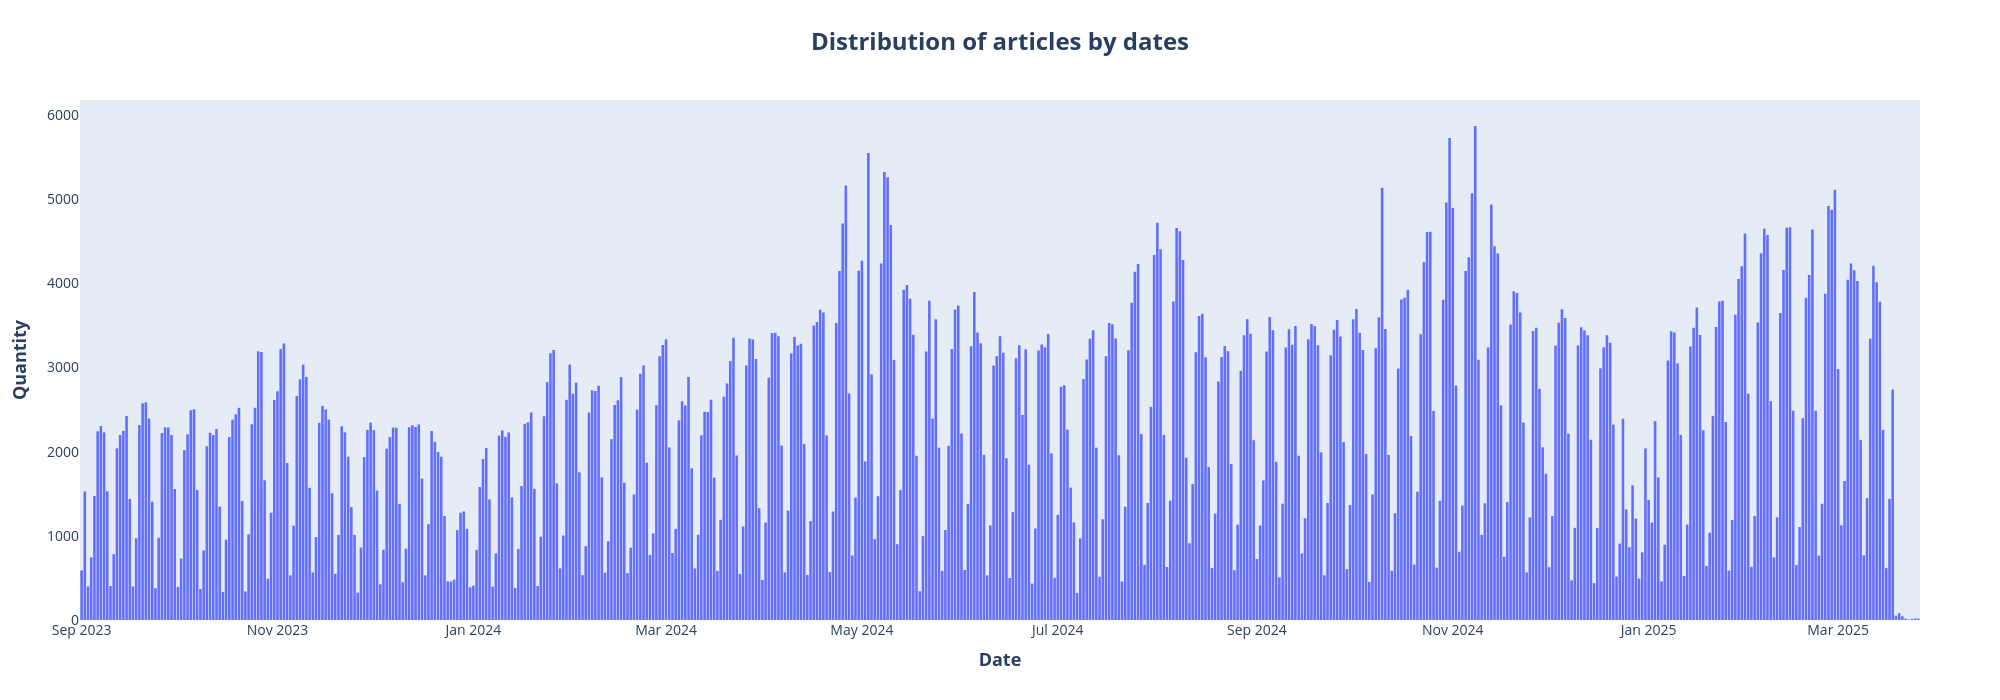
\includegraphics[width=1\linewidth]{img/articles_dist_by_dates.png}
    \caption{Распределение содержащихся в корпусе публикаций по датам.}
    \label{fig:dist_by_dates}
\end{figure}

\textbf{Распределение публикаций по датам.} На Рис. \ref{fig:dist_by_dates} видно, что количество публикаций
колеблется по дням с определённой периодичностью. Детальное изучение показало, что минимумы приходятся
на воскресные и праздничные дни, когда публикуется меньше финансовых новостей. Это естественно отражает
специфику рынка: в выходные и праздничные дни деловая активность снижается, поэтому и публикаций становится меньше.

\begin{figure}[H]
    \centering
    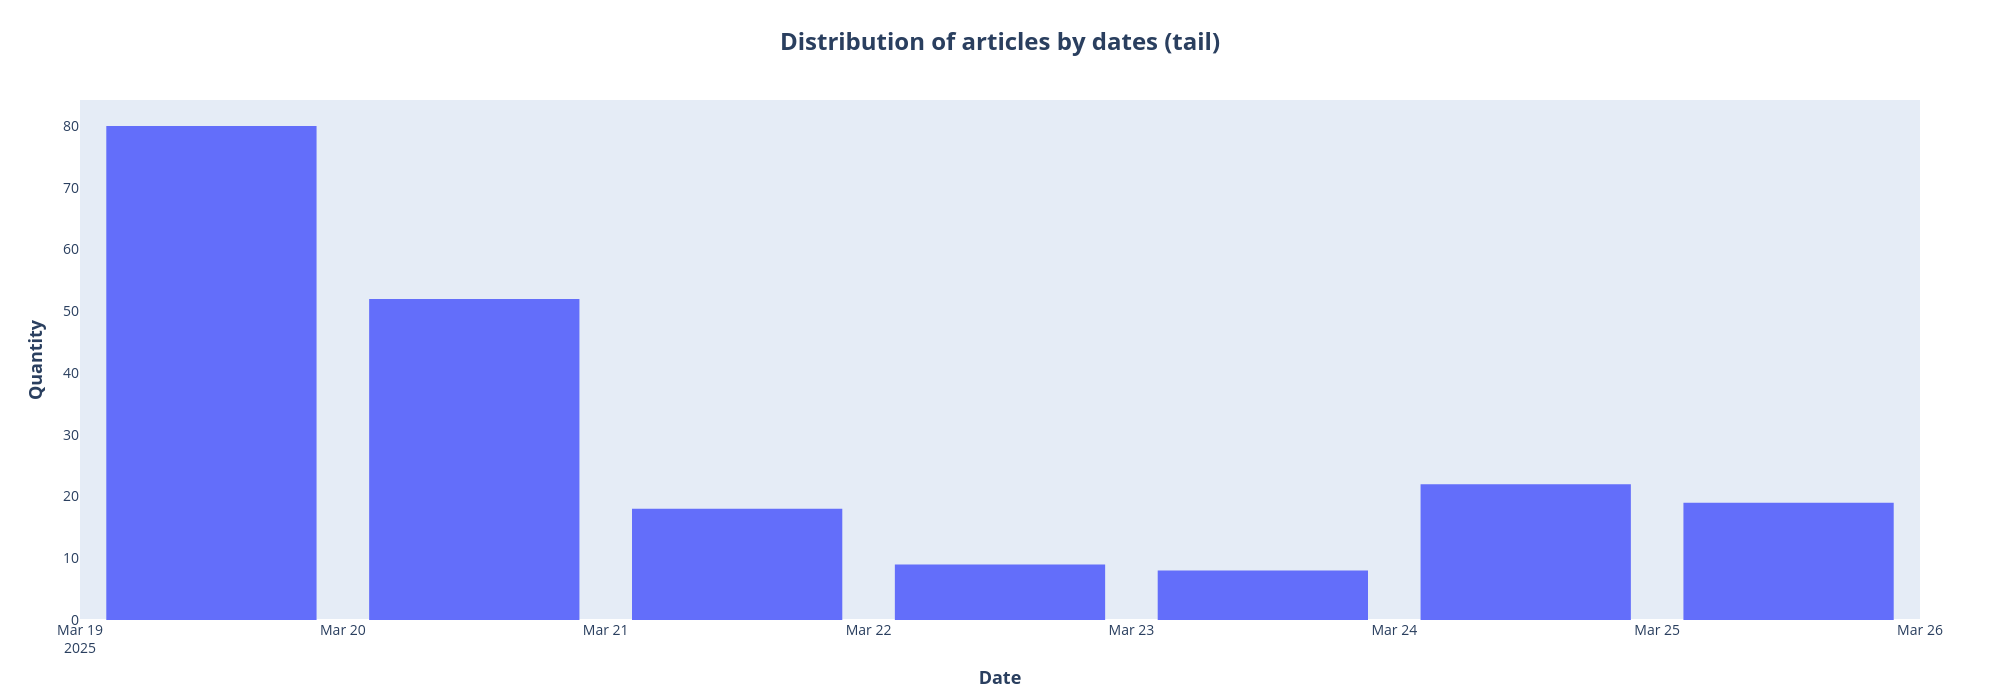
\includegraphics[width=1\linewidth]{img/articles_dist_by_dates_tail.png}
    \caption{\label{fig:dist_by_dates_tail}Распределение содержащихся в корпусе публикаций по датам (хвост).}
\end{figure}

При этом часть статей, по формальным признакам, выходит за границы периода сбора (1 сентября 2023 года --- 18 марта 2025 года).
На Рисунок \ref{fig:dist_by_dates_tail} показаны эти «хвостовые» публикации, численность которых слегка превышает 200 единиц.
Более детальный анализ установил, что публикации фактически были сделаны в установленный интервал, однако их содержание
редактировали или дополняли позже. В результате дата и время публикации на соответствующем сайте обновились, а старая версия
(со старой датой) утрачена. Если бы ссылки парсились не через неделю, а спустя несколько недель и более, таких случаев было
бы несколько больше.


С точки зрения краткосрочного прогнозирования рынка это обстоятельство может привести к искажению временных меток:
часть статей будто бы опубликована позже, чем на самом деле. Поэтому датасет может оказаться менее эффективен
в краткосрочных исследованиях, чем в средне- и долгосрочных (где сдвиг в пару дней уже не так принципиален).
Тем не менее, для данной работы это не играет критической роли, поскольку модель всё равно опирается лишь
на текст статьи и не учитывает точные временные метки публикаций.

\begin{figure}[H]
    \centering
    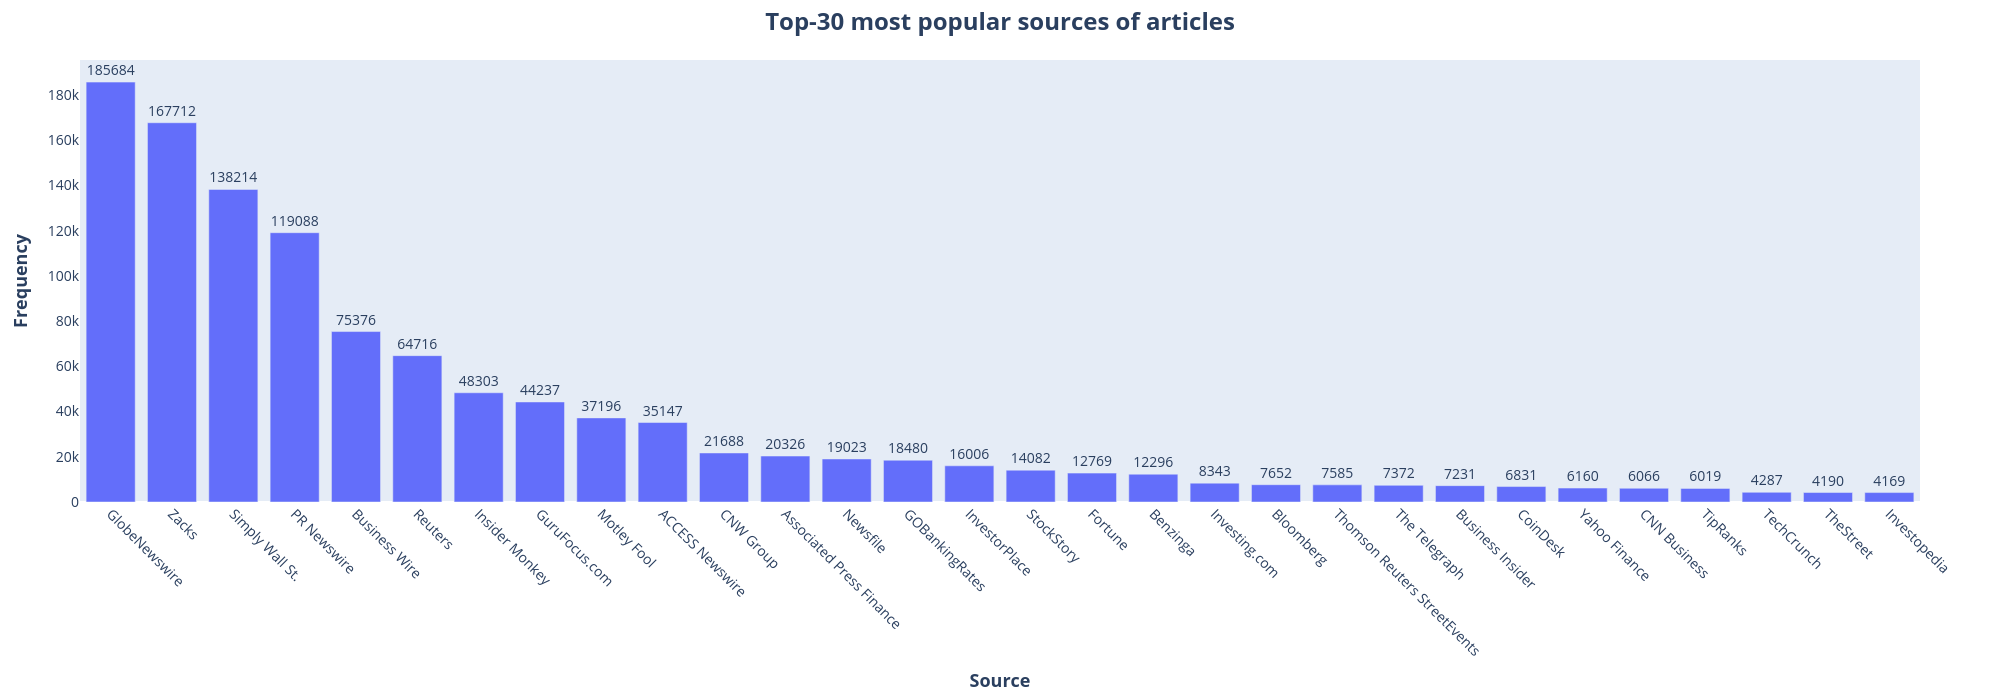
\includegraphics[width=1\linewidth]{img/top30_sources.png}
    \caption{\label{fig:dist_sources}30 наиболее популярных источников финансовых публикаций в корпусе.}
\end{figure}

\textbf{Новостные источники.} Рисунок \ref{fig:dist_sources} иллюстрирует распределение публикаций по 30 наиболее частым источникам.
Анализ показал, что преобладающая доля статей (потенциально 69.2\%) была опубликована полу-автоматизированными агрегаторами:
GlobeNewswire, Zacks, Simply Wall St., PR Newswire, Business Wire, GuruFocus.com, Motley Fool и др. Они фокусируются
на автоматическом сборе ключевых данных с различных ресурсов (регуляторы, официальные сайты компаний и т.п.), публикуя
пресс-релизы, краткие обзоры отчётов и приглашения на корпоративные мероприятия.

В топ-15 источников лишь некоторые можно условно считать «традиционными» новостными ресурсами, такими как Reuters,
Insider Monkey, CNW Group, Associated Press Finance, InvestorPlace. При этом за пределами топ-30 превалируют именно
классические издания, которые в основном публикуют авторские статьи. В реальности же размытая грань между авторскими
и полу-автоматическими материалами усложняет попытки чёткого разграничения.

По приблизительной оценке, из 1 300 000 статей около 900 000 (69.2\%) являются полу-автоматическими.
Это важный фактор для обучения языковой модели, поскольку:

\begin{enumerate}
    \item Качество таких материалов нередко ниже: тексты содержат артефакты, ломаются разметки и вставляются некорректные символы.
    \item Их объём велик, что, с одной стороны, даёт большую семплирующую способность, но с другой — затрудняет очистку и нормализацию без потери значимой информации.
\end{enumerate}

Тем не менее, даже «нечистые» тексты из агрегаторов несут полезную информацию о финансовом рынке и компаниях. Однако, крайне важно разработать корректные правила
очистки и предобработки (см. \hyperref[sec:data_prep]{Раздел 2.2.4}) текстов, чтобы не повредить их семантическую целостность.

Кроме того, и, что более важно, эти полу-автоматические тексты составляют примерно такое же общее количество токенов,
как и «авторские» статьи (30.8\%), несмотря на их количественное доминирование. Следовательно, при правильной обработке
данная группа полу-автоматических статей может дать значимый вклад в обучение языковой модели, не размывая значимость
«авторских» текстов.

\begin{figure}[H]
    \centering
    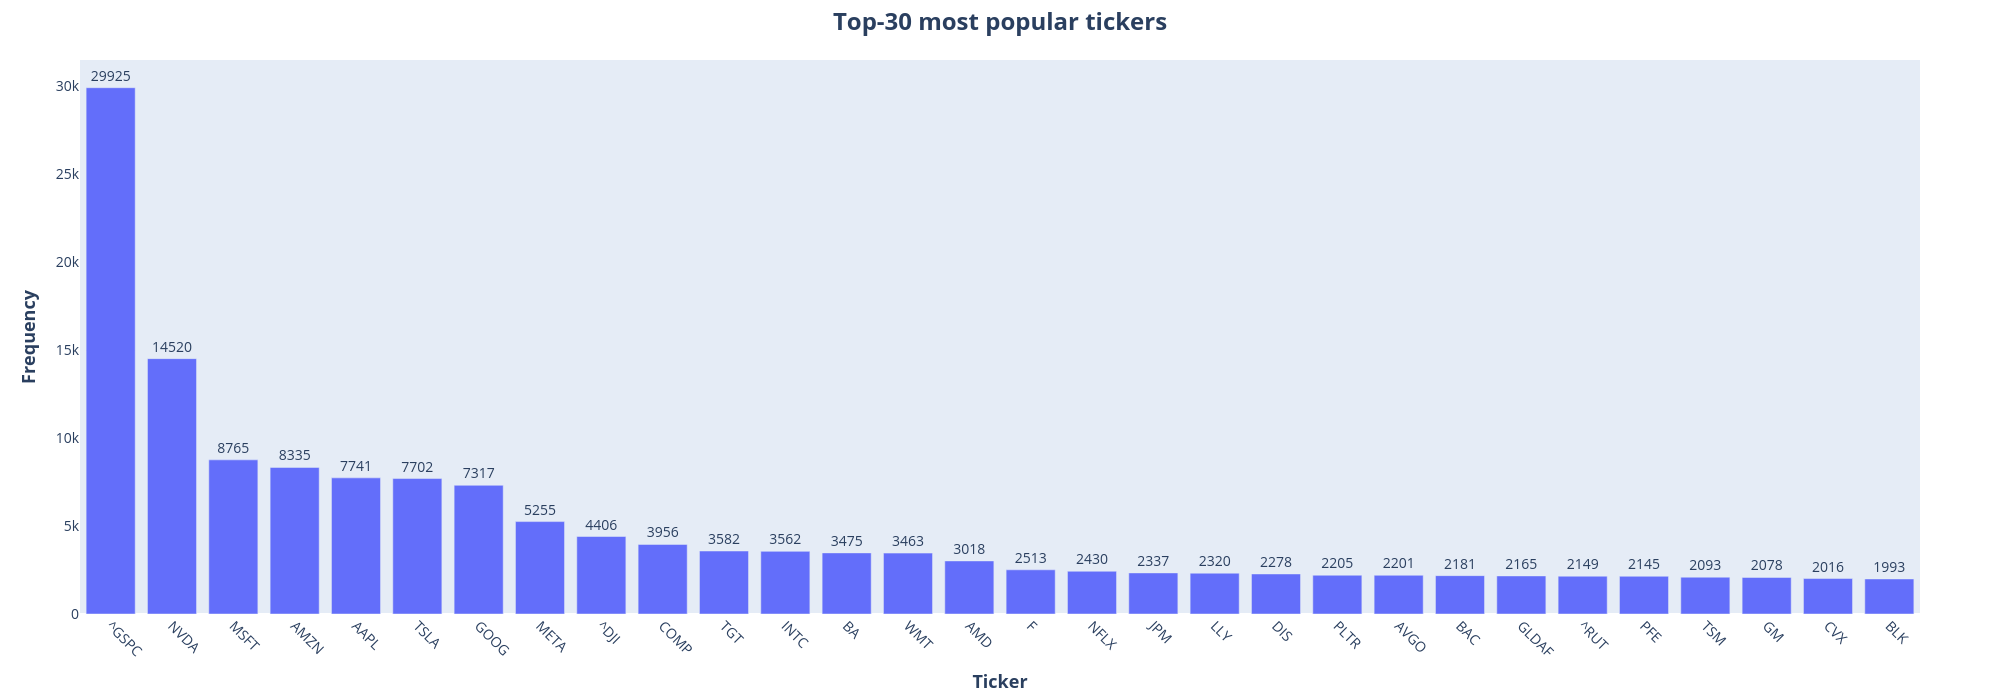
\includegraphics[width=1\linewidth]{img/top30_tickers.png}
    \caption{\label{fig:dist_tickers}30 наиболее частых тикеров в датасете.}
\end{figure}

\textbf{Анализ тикеров.} На Рисунке \ref{fig:dist_tickers} представлено распределение публикаций по 30 наиболее часто встречающимся
тикерам. Лидером является индекс S\&P 500, однако в выборку также попали Dow Jones и Russell 2000. Примечательно, что в топ-10
оказались главным образом IT-компании, причём с существенным отрывом лидирует Nvidia.

При этом около 574 000 (44,2\%) публикаций не содержат вообще никаких тикеров в описании статьи, которое находится
в шапке страницы. Более того, даже когда тикеры присутствуют, они могут отображать не все фактически упомянутые
в статье компании или индексы. Это говорит о том, что данный столбец в датасете, пусть и достаточно репрезентативен,
но не даёт полного покрытия всех потенциальных тикеров, и часть новостей формально «выпадает» из рассмотрения.
Следовательно, для задач, выходящих за рамки данной исследовательской работы стоит создать словарь терминов и наименований,
относящихся к каждому конкретному тикеру, а затем алгоритмически дополнить столбец с тикерами, используя соответствующие тексты.

\begin{figure}[H]
    \centering
    
\includegraphics[width=1\linewidth]{img/wordcloud.png}
    \caption{\label{fig:wordcloud}Облако слов, составленное по всем текстам, содержащимся в собранном корпусе.}
\end{figure}

\textbf{Качество текста.} На Рисунке \ref{fig:wordcloud} представлено облако слов, построенное по всему
корпусу собранных текстов. Из этой визуализации можно сделать следующие ключевые выводы:

\begin{enumerate}
    \item \textbf{Репрезентативность данных}. Облако демонстрирует широкий спектр финансовых терминов, что указывает на достаточную репрезентативность
    датасета в финансовой тематике. Это свидетельствует о том, что материал охватывает разнообразные аспекты рыночной деятельности и экономических событий.
    \item \textbf{Специфичность финансовой терминологии}. Распределение частот финансовых терминов существенно отличается от того,
    что наблюдается в популярных корпусах для обучения языковых моделей (например, English Wikipedia или BookCorpus).
    Это различие обуславливает необходимость проведения доменной адаптации DAPT для корректного обучения модели на специфических данных
    финансовой тематики.
    \item \textbf{Уровень шума и наличие нерелевантной информации}. Облако слов включает такие элементы, как «Zacks», «click»,
    «please», «free» и «source». Это указывает на значительное присутствие шумовых, рекламных или автоматически сгенерированных
    фрагментов, что требует разработки специальных методов очистки данных без нарушения семантической целостности текстов.
\end{enumerate}

Дополнительно можно отметить, что выявленные шум и рассеянность терминов могут негативно сказаться на качестве downstream-задач, таких как классификация
или извлечение эмбеддингов, если данные не будут корректно обработаны на этапе предобработки.

\textbf{Вывод}. Собранный датасет новостей характеризуется некоторыми особенностями. Во-первых, наблюдается ярко выраженная сезонность
публикаций --- минимумы приходятся на выходные и праздничные дни, также зафиксированы так называемые «хвостовые» статьи. Во-вторых,
анализ источников показывает, что около 69\% текстов поступают от полу-автоматизированных агрегаторов, что может усложнить процесс очистки
данных, поскольку такие источники нередко порождают тексты с нарушенной разметкой, встроенными артефактами и нерелевантной информацией.
Наконец, выяснено, что датасет обладает высокой вариативностью финансовой терминологии, но в то же время содержит значительный уровень шума,
что в совокупности подтверждает необходимость проведения доменной адаптации (DAPT) и разработки методов для эффективной очистки текстов.

С одной стороны, выявленные особенности (временные сдвиги, шум, доминирование полу-автоматизированных источников) могут
снижать пригодность датасета для краткосрочного прогнозирования или задач, требующих строгой временной разметки. С другой
стороны, для задач, ориентированных на семантическое содержание текста, данные проблемы не оказывают критического влияния.
Надлежащая предобработка, включающая очистку текстов и устранение нерелевантных элементов, позволит существенно повысить качество
обучаемой модели и расширить ее возможности для обобщения на различные типы публикаций.

\subsubsection{Предобработка данных}
\label{sec:data_prep}
После проведения локального и глобального анализов текстовых данных, в ходе которых были выявлены как шумовые
паттерны внутри отдельных документов, так и системные аномалии, свидетельствующие о нерепрезентативности некоторых
публикаций в корпусе в целом, был спроектирован многоэтапный потоковый пайплайн предобработки на лету с использованием
чанков по 100 000 публикаций. Ключевым ограничением при разработке решения стала ограниченность оперативной памяти: при
объёме исходного корпуса порядка 15 ГБ стандартные операции фильтрации и полного прохода по текстам требовали выделения
значительного константного буфера памяти. Это породило необходимость адаптации алгоритма к потоковой обработке порциями
фиксированного размера.

В ходе первого этапа каждый чанк загружался из хранилища и сразу подвергался первичной фильтрации: документы,
содержащие менее 100 символов, отбраковывались как недостаточно информативные. Эмпирически установленный порог
в 100 символов оказался достаточен для устранения «пустых» артефактов, возникающих из-за нестабильности разметки
на стороне источников. Так, на популярных площадках вроде Yahoo! Finance текст порой оказываются зашитым внутри
нетипичных HTML-тегов — например, в ‘<tbody>’ вместо привычного ‘<p>’ — что приводит к появлению почти полностью
пробельных записей или маркетинговых вставок в конце документа.

Следующим шагом реализован фильтр по заголовку: на его основе формализованы 66 правил, охватывающих как общие
шаблоны («Form 8», «Net Asset Value», «Holdings in company»), так и более таргетированные для шумных 12 источников
(например, в GlobeNewswire удалялись заголовки, содержащие «Declaration» или начинающиеся с «Key digital»). Такая
селекция гарантировала удаление публикаций, состоящих преимущественно из табличных данных или кратких заполнителей.

После нормализации всех видов пробельных символов — слияния подряд идущих пробелов или переносов строк в единичный
символ, замены неразрывных пробелов ‘\\xa0’ на стандартный пробел и унификации специальных знаков в тексте ---
применялись ещё 12 правил, направленных на отбраковку нерепрезентативных документов по содержанию основного тела
публикации. В частности, всё, что начиналось с маркера «(Repeat)», а также приветственные шаблоны специфичных
источников вроде «Dear madam, sir, please find hereunder the links» для GlobeNewswire, автоматически исключалось
из дальнейшей обработки.

Далее текст очищался от контактных данных и типовых футеров: ссылки, адреса электронной почты, а также фразы,
однозначно указывающие на конец документа («Forward-looking statements», «Contact Details»), либо нерепрезентативность
абзаца («Source:», «See More:», «Sponsored:»). Кроме того, из начала публикаций удалялись стандартные вводные фразы вроде
«The recommendations of Wall Street analysts» и «When deciding whether to buy, sell, or hold a stock, investors often
rely on analyst recommendations». Всего в различных группах было сформировано 92 правила очистки.

Такое агрессивное очищение текстов обуславливается тем, что отфильтрованные паттерны встречаются настолько часто,
что крайне негативно сказываются на кластеризации искусственно завышая метрику кластеризации. После проведенном
агрессивном очищении корпуса, метрика качества действительно уменьшилась, однако кластеры стали гораздо более
репрезентативными и основанными на семантике самой новости, а не ее источниках, маркетинговой и правовой информации
в текстах.

\begin{figure}[H]
    \centering
    
\includegraphics[width=1\linewidth]{img/prep_wordcloud.png}
    \caption{\label{fig:prep_wordcloud} Облако слов, составленное по всем по текстам, содержащимся в предобработанном корпусе.}
\end{figure}

В качестве валидации качества очистки текстов можно обратиться к облаку слов корпуса после предобработки (Изображение \ref{fig:prep_wordcloud}),
на котором отчетливо видно улучшение: отсутствуют такие слова, как 'forwardlooking', 'link', 'click', 'simply' (название источника Simply Wall St.) и другие.

Наконец, перед сохранением чанков происходила сортировка по дате публикации и удаление дубликатов на основе полного текста документа.
С учётом описанных операций объём корпуса сократился с 15,4 ГБ в формате CSV (8,6 ГБ в Parquet) до 5,9 ГБ (2,0 ГБ в Parquet): из 1 304 717
исходных записей осталось 1 267 416, то есть удалено было всего 2,8\% документов. Данный результат свидетельствует о высокой
доле шумов в тексте в собранном датасете и подчёркивает эффективность многоступенчатого потокового подхода к предобработке,
который сохраняет оперативную память и обеспечивает качественную очистку текстовых данных перед последующими этапами
тематического моделирования и анализа.


\subsection{Model Development}
\subsubsection{Извлечение векторных представлений}
После предобработки корпуса текстов и удаления фонового шума, для ускорения последующих этапов тематического моделирования,
включая обучение моделей понижения размерности и кластеризации, были извлечены их эмбеддинги.

Базовая модель ModernBERT не оптимальна для этой задачи, поскольку её векторные представления оказываются чрезмерно разреженными.
Высокая степень разреженности эмбеддингов ухудшает качество кластеризации, в частности методов, основанных на оценке плотностей
(например, DBSCAN). Несмотря на более высокую устойчивость HDBSCAN к различиям плотностей, разреженность всё равно негативно
сказывается на результатах кластерного разбиения.

Чтобы устранить указанную проблему, обычно применяют тонкую настройку модели под задачу STS. При этом модель получает на вход пару
текстов и возвращает оценку их сходства \parencite{MTEB2023}, чаще всего вычисляемую через косинусное расстояние (Формула \ref{eq:cos_dist}).

\begin{equation}\label{eq:cos_dist}
    D_{\cos}(\mathbf{u}, \mathbf{v})
    = 1 - \frac{\mathbf{u} \cdot \mathbf{v}}
                 {\|\mathbf{u}\|_2 \,\|\mathbf{v}\|_2}.
\end{equation}

Именно STS‑модели демонстрируют наиболее плотные и информативные эмбеддинги.

Так, для базовой модели ModernBERT было рассмотрено 2 тонко настроенные модели --- 'modernbert-embed' от Nomic AI \parencite{nomic2024}
и `gte-modernbert-base` от Alibaba \parencite{MGTE2023,MGTE2024}. Для оценки данных двух моделей был использован бенчмарк Massive
Text Embedding Benchmark (MTEB) \parencite{MTEB2023}, охватывающий восемь классов задач и 58 датасетов. По результатам:

\begin{itemize}
    \item В задаче кластеризации на 12 датасетах 'gte-modernbert-base' превзошла 'modernbert-embed' на 1.5 процентных пункта (44.98\% против 44.47\%).
    \item В задаче STS на 10 датасетах их результаты близки (81.78\% и 81.57\% соответственно).
    \item В среднем по всем восьми задачам на 56 датасетах 'gte-modernbert-base' опережает 'modernbert-embed' на 1.76 процентных
    пункта (64.38\% против 62.62\%).
\end{itemize}

В связи с этим для извлечения эмбеддингов была выбрана модель gte-modernbert-base из библиотеки 'sentence\_transformers' \parencite{SBERT2019}.
При получении эмбеддингов для всего документа вместо токена [CLS] применялась более продвинутая техника --- Mean Pooling, которая заключается
в усреднении значений эмбеддингов по всем токенам последовательности (Формула \ref{eq:mean_pooling}).

\begin{equation}\label{eq:mean_pooling}
    \mathbf{h_{mean}}=\frac{1}{T}\sum^T_{t=1}\mathbf{h}_{t}.
\end{equation}

где $T$ — длина токенизированной последовательности, а $\mathbf{h}_t$ — эмбеддинг $t$-го токена.

Для оптимизации скорости обучения моделей понижения размерности и кластеризации,
эмбеддинги предварительно приводились к единичной $L_2$-норме (Формула \ref{eq:l2_norm}):

\begin{equation}\label{eq:l2_norm}
    \widehat{\mathbf{u}}
    = \frac{\mathbf{u}}{\|\mathbf{u}\|_2},
    \qquad
    \|\mathbf{u}\|_2 = \sqrt{\sum_{i=1}^{n} u_i^2}.
\end{equation}

Подобная предобработка позволяет пользоваться GPU-оптимизированной евклидовой метрикой расстояния (Формула \ref{eq:euclidean}) при обучении модели DR,
не повторяя при этом на каждой итерации оптимизации гиперпараметров вычисление $L_2$-нормы, которое происходит при вычислении метрики косинусного расстояния.

\begin{equation}\label{eq:euclidean}
    D_{2}(\mathbf{u}, \mathbf{v})
    = \|\mathbf{u} - \mathbf{v}\|_2
    = \sqrt{\sum_{i=1}^{n} \bigl(u_i - v_i\bigr)^2}.
\end{equation}

Таким образом, после вычисления $L_2$-нормы и евклидова расстояния, мы, на самом деле, в некотором смысле можно считать, что мы работаем с косинусным расстоянием,
так как приведенная мера становится монотонно связанной с косинусным и отражает тот же порядок близости точек (Формула \ref{eq:euclidean_after_l2_norm}),
однако все вычисления ускоряются за счет GPU-оптимизации.

\begin{equation}\label{eq:euclidean_after_l2_norm}
    D_{2}\bigl(\widehat{\mathbf{u}}, \widehat{\mathbf{v}}\bigr)
    = \bigl\|\widehat{\mathbf{u}} - \widehat{\mathbf{v}}\bigr\|_2
    = \sqrt{2\,\bigl(1 - \widehat{\mathbf{u}}\!\cdot\!\widehat{\mathbf{v}}\bigr)}.
\end{equation}

Для построения и обучения алгоритмов понижения размерности и кластеризации была сформирована
тренировочная выборка из 200 000 эмбеддингов и сопутствующих метаданных, что составляет приблизительно
16\% от всего корпуса. Такой объем обучающей подвыборки был выбран, исходя из доступных вычислительных
ресурсов. Так, 200 000 эмбеддингов использовались для подбора оптимальных гиперпараметров,
а остальные 1 050 000 эмбеддингов были зарезервированы для этапов валидации и инференса.
При этом, перед инференсом конвейер моделей понижения размерности и кластеризации были обучены
на всем корпусе с линейным увеличением значений гиперпараметров для алгоритма HDBSCAN, выбор которого
обуславливается в \hyperref[sec:drc]{Секции 2.3.2}.

Кроме того, при извлечении эмбеддингов была задействована смешанная точность (float16) и ускоренный
механизм внимания FlashAttention \parencite{flash2022attention}, что существенно сократило требования
к вычислительным ресурсам и время обработки.

\subsubsection{Модели понижения размерности и кластеризации}
\label{sec:drc}
Итак, после формирования выборки эмбеддингов мы приступили к экспериментам с моделями DR и кластеризации,
проводя их совместную оптимизацию. Такой подход обусловлен многокритериальным характером задачи: требуется
не только сохранить структурные (глобальные) и локальные взаимосвязи из исходного 768-мерного пространства,
но и обеспечить разделимость («кластерность») эмбеддингов в низкоразмерной проекции, пригодной для визуализации на плоскости.

В качестве ключевых условий было обозначено:

\begin{enumerate}
    \item Сохранение кластерной структуры. Эмбеддинги после понижения размерности должны оставаться разделимыми,
    то есть сохранять группировку по смыслу и тематике.
    \item Готовность к двумерной визуализации. Итоговое пространство должно быть пригодно для наглядного
    отображения на плоскости без потери интерпретируемости.
\end{enumerate}

Для одновременного поиска оптимальных гиперпараметров выбора алгоритмов понижения размерности
и методов кластеризации использовался единый мета‑процесс.

В качестве критерия оптимальности был принят индекс DBCV, поскольку он не предполагает заранее заданной
формы кластеров (в отличие от индексов, ориентированных на сферические или эллипсоидальные структуры)
и эффективно оценивает плотностные методы кластеризации.

В качестве основы был выбран алгоритм HDBSCAN \parencite{HDBSCAN2013}, отвечающий двум важным требованиям:

\begin{itemize}
    \item Отсутствие предположений о форме кластеров. В отличие от K‑Means HDBSCAN не предполагает,
    что кластеры являются гауссовыми сферами, что критически для представления тем.
    \item Иерархическая и плотностная природа. Позволяет выявлять как крупные тематические группы,
    так и мелкие, высококонцентрированные ниши.
\end{itemize}

Кроме того, благодаря реализации на GPU, HDBSCAN показал высокую скорость обработки
как больших выборок, так и высокоразмерных данных.

В контексте алгоритма HDBSCAN для оптимизации рассматривается несколько ключевых гиперпараметров.
Минимальное число соседей --- количество точек в окрестности, необходимое для признания точки «ядром» кластера.
Минимальный размер кластера --- число наблюдений, определяющее порог для формирования кластера,
что позволяет учитывать редкие, узкотематические группы.

 В ходе пилотных экспериментов было обнаружено, что одновременно существуют плотные области («горячие темы»)
 и редкие, но значимые по содержанию кластеры. При малом минимальный размер кластера удаётся захватывать
 редкие темы, однако возрастает число микрокластеров, разделение между которыми семантически не всегда оправдано.

 Для смягчения этой проблемы рассматривалась техника объединения кластеров по порогу $\epsilon$ \parencite{HDBSCAN2020cluster_selection_epsilon}, позволяющая
 консолидировать соседние микрокластеры в высококонцентрированных регионах. Однако такой подход усложняет
 инференс модели: при появлении новых наблюдений $\epsilon$‑объединение не может быть учтено, что вынуждает
 полностью переобучать модель.

 Так как исследование ставит своим приоритетом практичность, было принято решение отказаться от использования
 $\epsilon$, но использовать меньшие значения минимального размера кластера, принимая некоторую фрагментацию,
 но сохраняя возможность последующей интерпретации и агломерации кластеров на более высоком уровне иерархии.

 Ещё один гиперпараметр --- метод выделения кластеров --- определяет, будут ли они формироваться на основе «избытка массы» или «листьев дерева».
 Практика показала, что второй вариант даёт более мелкозернистые и однородные группы, что и было избрано для окончательной настройки.

 Таким образом, на финальной стадии оптимизации HDBSCAN оставлены лишь два подлежащих настройке параметра: минимальное
 число соседей и минимальный размер кластера.

 Также стоит отметить, что в архитектуре, описанной в \hyperref[sec:architecture]{Разделе 3.3},
 планируется фиксированное количество кластеров для статичного числа экспертов,
 поэтому в качестве базовой реализации используется именно HDBSCAN из cuML,
 а не его адаптивная версия \parencite{HDBSCAN2022adaptive}.

 Переходя к алгоритмам понижения размерности, для предварительного отбора рассматривались
 t-SNE, PCA, UMAP, TriMap и PaCMAP, причём ключевыми критериями были точность, возможность
 балансировать отображения локальных и глобальных отношений и скорость обучения. Исходя из опыта
 других исследователей в качестве базового алгоритма для сравнения был выбран UMAP \parencite{BERTopic2022}.

Так, исключён из-за недостаточной производительности на больших объёмах данных. PCA рассматривался как
быстрое глобальное приближение, но для конечного понижения размерности не обеспечивает локальную точность.
Тем не менее, был проведён эксперимент с предварительным применением PCA перед основным алгоритмом,
направленный на ускорение вычислений. Эксперимент показал, что пайплайн PCA + UMAP уступает по индексу
DBCV «чистому» UMAP примерно на 37\%, что сделало применение PCA неоправданным.

Дальнейшее сравнение UMAP, TriMap и PaCMAP продемонстрировало схожую точность при проекции в промежуточные размерности,
однако для окончательной двумерной визуализации PaCMAP оказался предпочтительнее за счёт более равномерного распределения
кластеров на плоскости. Тем не менее, поскольку для кластеризации на промежуточном этапе была важна возможность GPU-ускоренной
оптимизации и проверенная устойчивость, выбор пал на UMAP реализованном в cuML \parencite{cuml2020machine}.

\subsubsection{Оптимизация гиперпараметров}

После этапа инициализации моделей последовала комплексная оптимизация гиперпараметров, затрагивающая
семь ключевых параметров: пять для UMAP (число соседей 'n\_neighbors', размер выходного пространства 'n\_components',
параметры 'min\_dist' и 'spread', коэффициент 'negative\_sample\_rate') и два для HDBSCAN ('min\_cluster\_size' и 'min\_samples').
В качестве фреймворков для поиска оптимума были апробированы Ray Tune \parencite{raytune2018liaw} и Optuna \parencite{optuna2019akiba},
причём акцент был сделан на ресурсно-ориентированном подходе, где «ресурсом» выступал размер обучающей подвыборки.
Экспериментально были выбрано 5 этапов обучения с долями от 1.5\% до 10\% общего корпуса, что позволило
оценить масштабируемость методов и устойчивость полученных гиперпараметров.

В контексте Ray Tune применялась схема Байесовской оптимизации с HyperBand (BOHB)
\parencite{TPEandBO2011bergstra, BOHB2018falkner, hyperband2018li, HPOoverview2015shahriari},
однако она не обеспечила должного соотношения скорости и качества при работе с UMAP/HDBSCAN.
Переключившись на Optuna, были реализованы три разновидности «прунеров» --- механизмы
для досрочного отсечения бесперспективных комбинаций при наращивании ресурса.
Первый, 'AdaptiveStablePercentilePruner', удалял худшие по заранее заданному перцентилю
в каждом шаге ресурса, второй, 'CustomPatientPruner', минимизировал риск преждевременного исключения,
отсекая комбинации после $n$ последовательных неудачных шагов с приростом менее $\delta$, а третий,
'NormalPruner', использовал Z-статистику (Формула \ref{eq:z_score}) и заданный перцентиля стандартного
нормального распределения ($\mathcal{N}(0, 1)$).

\begin{equation}\label{eq:z_score}
    z\text{-score}=\frac{m - \mathbb{E}[M]}{\mathbb{V}[M]},
\end{equation}

где $m$ --- текущая метрика и $M$ --- распределение метрик на данном этапе.

Метрикой оценки в ходе итераций стал взвешенный кумулятивный DBCV-индекс (WCDBCV):

\begin{equation}
    WCDBCV_j=\frac{1}{j\sum_{i=1}^jp_i} \sum_{i=1}^j p_i \cdot DBCV_i,
\end{equation}

где $j$ — текущий этап ресурса, а $p_i$ — доля выборки, использованная на $i$-м шаге.

Из всех сочетаний наилучшую эффективность продемонстрировал алгоритм Древовидной оценка Парсена (TPE)
\parencite{TPE2023watanabe, TPEandBO2011bergstra, HPOoverview2015shahriari} в связке с 'AdaptiveStablePercentilePruner',
однако прирост качества оказался недостаточно существенным относительно возросших вычислительных затрат.
В связи с этим последующий поиск гиперпараметров был выполнен без использования прунинга.
В качестве глобальной стратегии применялся классический TPE с 400 испытаниями, из которых половина
выполнялась в «разминочном» режиме случайных конфигураций. Для локальной донастройки возникших
перспективных областей пространства гиперпараметров использовалась адаптивная эволюционная стратегия
(CMAES) \parencite{restartCMAES2005auger, CMAES2024nomura} с механизмом повторного старта IPOP, адаптивной
скоростью обучения и предварительным «тёплым запуском» на базе 15 лучших комбинаций, найденных
на этапе глобальной оптимизации \parencite{CMAES2024nomura, lrCMAES2023nomura, restartCMAES2005auger, warmCMAES2021nomura}.
Бюджет локальной фазы составил 250 испытаний, что обеспечило глубокий поиск вокруг уже высокоэффективных конфигураций.

В результате такого двухуровневого подхода --- сначала широкого исследования методом TPE, затем углублённого
локального поиска CMAES --- удалось сбалансировать широту и глубину оптимизации, повысив устойчивость конвейера моделей.

\subsection{System Development}
\label{sec:sys_dev}
После завершения этапа семантической кластеризации и построения тематических групп,
необходимо обработать сформированные кластеры на лингвистическом уровне. В тематическом
моделировании качество представлений тем является ключевым для интерпретации тем,
передачи результатов и понимания закономерностей. Так, необходимо убедиться,
что каждое множество документов действительно характеризуется уникальным набором
ключевых терминов и не содержит артефактов неправильной сегментации. Данная валидация
выходит за пределы чисто метрических оценок и требует эмпирического, «человеческого»
взгляда на то, какие слова действительно определяют содержание темы. В контексте
неразмеченного корпуса такая проверка особенно важна: без исходных меток о тематике
единственным источником информации о семантической однородности кластеров остаётся
текст самой публикации. Более того, существует необходимость в присвоении названий
каждому из кластеров, поэтому крайне важно разработать пайплайн репрезентации тем.

С другой стороны, результатом кластеризации являются метки нижнего уровня, а в контексте
системы подразумевается иерархический подход к репрезентации тем, что ведет к необходимости
извлечения из текущей модели дополнительной информации и ее пост-обработки.

Для упрощения и формализации процесса в FinABYSS был реализован специализированный пайплайн
репрезентации тем, основанный на следующих инструментах:





\begin{itemize}
    \item BERTopic --- для удобства и упрощения процесса обработки лингвистических признаков,
    визуализации взвешенных частот слов, а также построения иерархии.
    \item OpenAI API --- для автоматизации разметки полученных кластеров на основе их лингвистических признаков.
    \item DataMapPlot для упрощения работы с графическим интерфейсом и создания интерактивной семантической карты.
    \item Собственная реализация:
    \begin{itemize}
        \item над BERTopic --- для реализации возможности выбора определенного количества иерархических тематических уровней.
        \item между BERTopic и OpenAI --- для реализации возможности присвоения тематических названий на основе
        лингвистических признаков на более высоких иерархических уровнях, нежели только на самом нижнем.
        \item между BERTopic и DataMapPlot — для тонкой настройки как статической, так и интерактивной семантической карты.
    \end{itemize}
\end{itemize}

Таким образом, первым этапов в пайплайне стала векторизация текстов, то есть приведение их к матричному виду.
С этой целью использовался 'CountVectorizer' из библиотеки 'sklearn', который был настроен настроенная
на извлечение униграмм и биграмм. Это полезно для более точной репрезентации тем, так как ведет к рассмотрению
таких терминов как “central bank”, “monetary policy” и “New York” и совместно, а не отдельно по словам..


Отныне, слова в контексте документов такие уни- и биграммы будут называться <<терминами>> для предотвращения
путаницы, так как, на самом деле, в контексте разработанной системы рассматриваются не слова, а $n$-граммы,
то есть короткие последовательности из $n$ слов.

Также на основе свободного англоязычного словаря стоп-слов \parencite{nothman2018stop} был настроен этап
фильтрации артиклей, предлогов, местоимений, союзов и других частей речи, мешающих отбору по-настоящему
репрезентативных терминов.

Наконец была настроена минимальная частота термина в документе для его включения в матрицу.
Несложно представить ситуацию, когда определенный термин встречается во всех документах только
один раз. Маловероятно, что данный термин отражает определенную тематику. С другой стороны,
в корпусе собрано более миллиона статей и, если не установить минимальную частоту термина,
матрица станет огромной и непрактичной в использовании. Поэтому термины, появляющиеся менее
15 раз во всём корпусе, отсекаются как статистически нерепрезентативные.

Наконец, система подразумевает функционирование в режиме реального времени, поэтому принципиально
важно уметь инкрементально обновлять матрицу терминов, для этого была использована онлайн версия
'CountVectorizer' --- 'OnlineCountVectorizer'.

После формирования матрицы терминов, необходимо сгруппировать их по тематическим кластерам
и определить релевантность терминов для каждой тематической группы, чтобы в дальнейшем,
на основе наиболее репрезентативных терминов сгенерировать названия кластеров.

Частота термина, обратная частота документа (Term Frequency Inverse Document Frequency, TF-IDF)
и Best Match (BM-25) являются аддитивными функциями релевантности. Они используются в большинстве
поисковых систем как основные метрики релевантности. Обе метрики показывают релевантность документа.
Чем выше значение метрик, тем более релевантен документ. При этом, важно отметить, что само значение
метрик не имеет какой-либо значимой интерпретации, кроме как относительная разность релевантности
документов или терминов друг с другом.

В контексте поисковых систем метрика отражает релевантность документа или термина поисковому запросу,
но в текущей системе используется модифицированная TF-IDF метрика, которая выражает релевантность
термина, не по отношению к запросу, а по отношению к теме.

Такая метрика, называется c-TF-IDF \parencite{BERTopic2022}. Лучше всего ее можно объяснить, как формулу TF-IDF принятую для всей
темы, в целом. То есть все документы внутри темы не рассматриваются по-отдельности, а объединяются в один
большой документ, на основе которого происходит подсчет. Так, c-TF-IDF учитывает то, что отличает документы
в одном тематическом кластере от документов в другом.

Таким образом, мы сначала извлекаем частоту термина $x$ в тематическом кластере $c$, которому и принадлежит
термин $x$. В результате получается представление $tf$ на основе классов. А для того, чтобы учесть различия
в размере тематических кластеров, по полученным частотам вычисляется $L_1$-норма.

Затем, вычисляется логарифм суммы единицы и частного от деления среднего количества слов в каждом
из тематических кластеров на частоту слова $x$ во всех кластерах. Так, получается представление $idf$,
которое помогает определить насколько данное слово $x$ редко встречается среди всех остальных классов.
Единица нужна для того, чтобы логарифм всегда был положительным.

Наконец, как и в случае с обычным TF-IDF, полученные репрезентации $tf$ и $idf$ перемножаются
(Формула \ref{eq:c_tf_idf}):

\begin{equation}\label{eq:c_tf_idf}
    w_{x, c} =
    ||tf_{x, c}||_1
    \times
    \log\Bigg(
        1 + \cfrac{
            \frac{1}{||\mathbb{C}||}\sum_{i \in \mathbb{C}}||\mathbb{X}_i||
        }{
            \sum_{i \in \mathbb{C}}x
        }
    \Bigg),
\end{equation}

где $w_{x, c}$ --- релевантность терма $x$ тематическому кластеру $c$,
$\mathbb{X_i}$ --- множество всех термов в тематическом кластере $i$.

Тем не менее, вместо классической формулы c-TF-IDF, было принято решение использовать
ее модифицированный аналог. Некоторые слова или термины встречаются слишком часто
в каждой из тем, однако не считаются типичными стоп-словами для исключения из текста.
Чтобы сгладить самые частые термины в теме, в системе применяется нормализация частот
терминов, то есть извлекается квадратный корень из $tf$, после применения схемы взвешивания.

С другой стороны, несмотря на то, что собранный финансовый корпус велик, он может
не вполне исчерпывающе отражать все лексическое изобилие генеральной совокупности.
Поэтому, для более стабильного результата, к $idf$ было применено преобразование BM-25.
Итоговая формула релевантности выглядит следующим образом:

\begin{equation}
    w_{x, c} =
    \sqrt{||tf_{x, c}||_1}
    \times
    \log\Bigg(
        1 + \cfrac{
            \frac{1}{||\mathbb{C}||}\sum_{i \in \mathbb{C}}||\mathbb{X}_i|| - \sum_{i \in \mathbb{C}}x + 0.5
        }{
            \sum_{i \in \mathbb{C}}x + 0.5
        }
    \Bigg),
\end{equation}

Коэффициенты $0.5$ основаны на подгонке под теоретически более чистую форму.
Такая форма дает меньший вес слишком часто встречающимся терминам.

В итоге, мы получаем для каждого из тематических кластеров мешки слов, которые
достаточно репрезентативно отражают лексическое богатство каждой темы. Тем не менее,
в мешках слов все еще могут присутствовать некоторые не совсем репрезентативные слова
или же мешок может быть излишне однородным. Данные проблемы могут негативно сказаться
на процессе генерации названий тем, поэтому при разработке системы был предусмотрен
более сложный пайплайн, который добавляет еще 2 шага перед финальной репрезентацией.

Первый шаг заключается в семантическом сравнении наиболее репрезентативных слов,
с наиболее репрезентативными документами. Сначала из мешка слов извлекается 30 наиболее
репрезентативных терминов, а из самого тематического кластера --- 5 наиболее репрезентативных
документов. Затем, мы собираем уже извлеченные эмбеддинги по соответствующим документам,
и при помощи той же эмбеддинговой модели —-- 'gte-modetnbert-base' --- извлекаем эмбеддинги
из выбранных терминов. После чего, мы сравниваем эмбеддинги терминов-кандидатов с наиболее
репрезентативными документами и ранжируем их по полученному значению метрики косинусного расстояния.

На втором шаге мы применяем алгоритм Максимальной Предельной Релевантности (Maximaxl Marginal Relevance,
MMR) --- это техника для реферирования по запросу, которая максимизирует похожесть фрагментов ответа
на запрос и минимизирует схожесть с уже выбранными в ответ фрагментами. Аналогично TF-IDF, в контексте
текущей системы рассматривается не запрос, а термин. То есть мы максимизируем внутреннее разнообразие
наиболее репрезентативных теме терминов. MMR вычисляется по следующей формуле:


\begin{equation}\label{eq:mmr}
    MMR =
    \argmax_{
        t_i \in \mathbb{R} \setminus \mathbb{S}
    }[
        \lambda(sim_1(t_i,\mathbb{C})) - (1 - \lambda)\max_{t_j \in \mathbb{S}}(sim_2(t_i, t_j))
    ],
\end{equation}

где $\mathbb{T}$ --- тема, для которой рассчитывается $MMR$, $\mathbb{R}$ --- множество всех терминов $t_i$ --- рассматриваемый термин,
а $\mathbb{S}$ — множество уже выбранных терминов. Получается, что мы ищем новый термин из $\mathbb{R} \setminus \mathbb{S}$ так,
чтобы он был максимально похож на тему, но минимально на на уже присутствующие в мешке слов термины. В Формуле \ref{eq:mmr}
коэффициент $\lambda$ является гиперпараметром и балансирует похожесть терминов на тему с непохожестью терминов друг с другом.
Чем меньше $\lambda$, тем термины менее похожи друг на друга, а чем больше, тем похожее термины на тему.

Так, у нас получается максимально репрезентативный набор терминов, относительно которых мы уже можем генерировать названия тем.
Непосредственно для генерации тем в системе предусмотрено использование text2text моделей. Конкретно в текущей реализации
использовалась модель GPT-4o, для которой был задан соответствующий промпт с инструкциями.
Модель использовалась с помощью OpenAI API. А все сгенерированные метки позднее были провалидированы вручную.

Наконец, заключительным этапом является визуализация семантической карты. Визуализация была выполнена
в двух форматах: в статичном --- для работы и презентации, и в интерактивном --- для функционирования системы.
Визуализация осуществлялась при помощи Python-библиотеки DataMapPlot, а также кастомных дополнений на HTML,
CSS и JavaScript. Также на системном уровне были разработаны функциональности для поиска по текстам,
построения облака слов, фильтрации по источникам, активам, дате публикации и другим количественным признакам.

    % Третья результирующая глава
    \newpage
    \section{РАЗУЛЬТАТЫ}
    \label{sec:results}
    \subsection{Invented Architecture}
\label{sec:architecture}
\subsubsection{Обзор}

В рамках данного исследования была разработана архитектура предиктивной системы нового поколения.
Основное внимание в настоящей работе уделено созданию системы тематического моделирования и аналитического
интерфейса для финансовой предметной области. Логичным продолжением станет построение интерпретируемой
и эффективной модели прогнозирования на основе тематической тональности финансовых публикаций
(новостных статей, пресс‑релизов, постов, транскриптов и др.). Таким образом, настоящая работа
не только демонстрирует принципы функционирования базового модуля, но и формулирует видение того,
каким образом можно расширить её возможностями предсказания цен активов.

Предложенная архитектура опирается на доказавшие свою надёжность подходы смешанного прогнозирования ---
сочетание сверточных и рекуррентных нейронных сетей (CNN-LSTM) \parencite{Hochreiter1997LSTM, CNN1998lecun, CNN_LSTM2020finance}.
Это решение позволяет одновременно учитывать глобальные долгосрочные тенденции (например, общий тренд рынка)
и локальные краткосрочные паттерны (такие как «голова и плечи», «двойное дно» и другие структуры,
обусловленные поведенческой экономикой).

При этом важно помнить о разнообразии исходных данных. Для прогнозирования обычно используют биржевые метрики
(OHLCV и т.п.) и производные технические индикаторы (RSI, MACD и др.).
В нашем исследовании к ним добавляются текстовые данные как внебиржевой источник. В дальнейшем в
качестве дополнительных модальностей могут быть привлечены графовые представления связей, изображения,
аудио‑ и видеозаписи. Таким образом, на текущем этапе мы работаем с тремя модальностями, каждая из которых
несёт самостоятельную смысловую нагрузку и способна объяснить динамику цен независимо, но их взаимодействие
может как усиливать полезный сигнал, так и вносить шум.

В данном исследовании архитектура была построена на основе CNN-LSTM с использованием медленного слияния.
Основной инженерный вызов состоял в согласовании пространственно‑временных форм признаков разных модальностей.
Для решения этой задачи в архитектуру введён Механизм Кэширования Признаков (Feature Caching Mechanism, FCM),
который синхронизирует тональностные векторы текстовой модальности с биржевыми временными рядами.

Дополнительно текстовая ветвь подвергается предобработке: на основе разработанной системы тематического
моделирования вычисляются тематические тональности публикаций. Это позволяет получить специализированные
оценки по каждой теме, что даёт преимущество перед использованием единой общей тональности.


\begin{figure}[H]
    \centering
    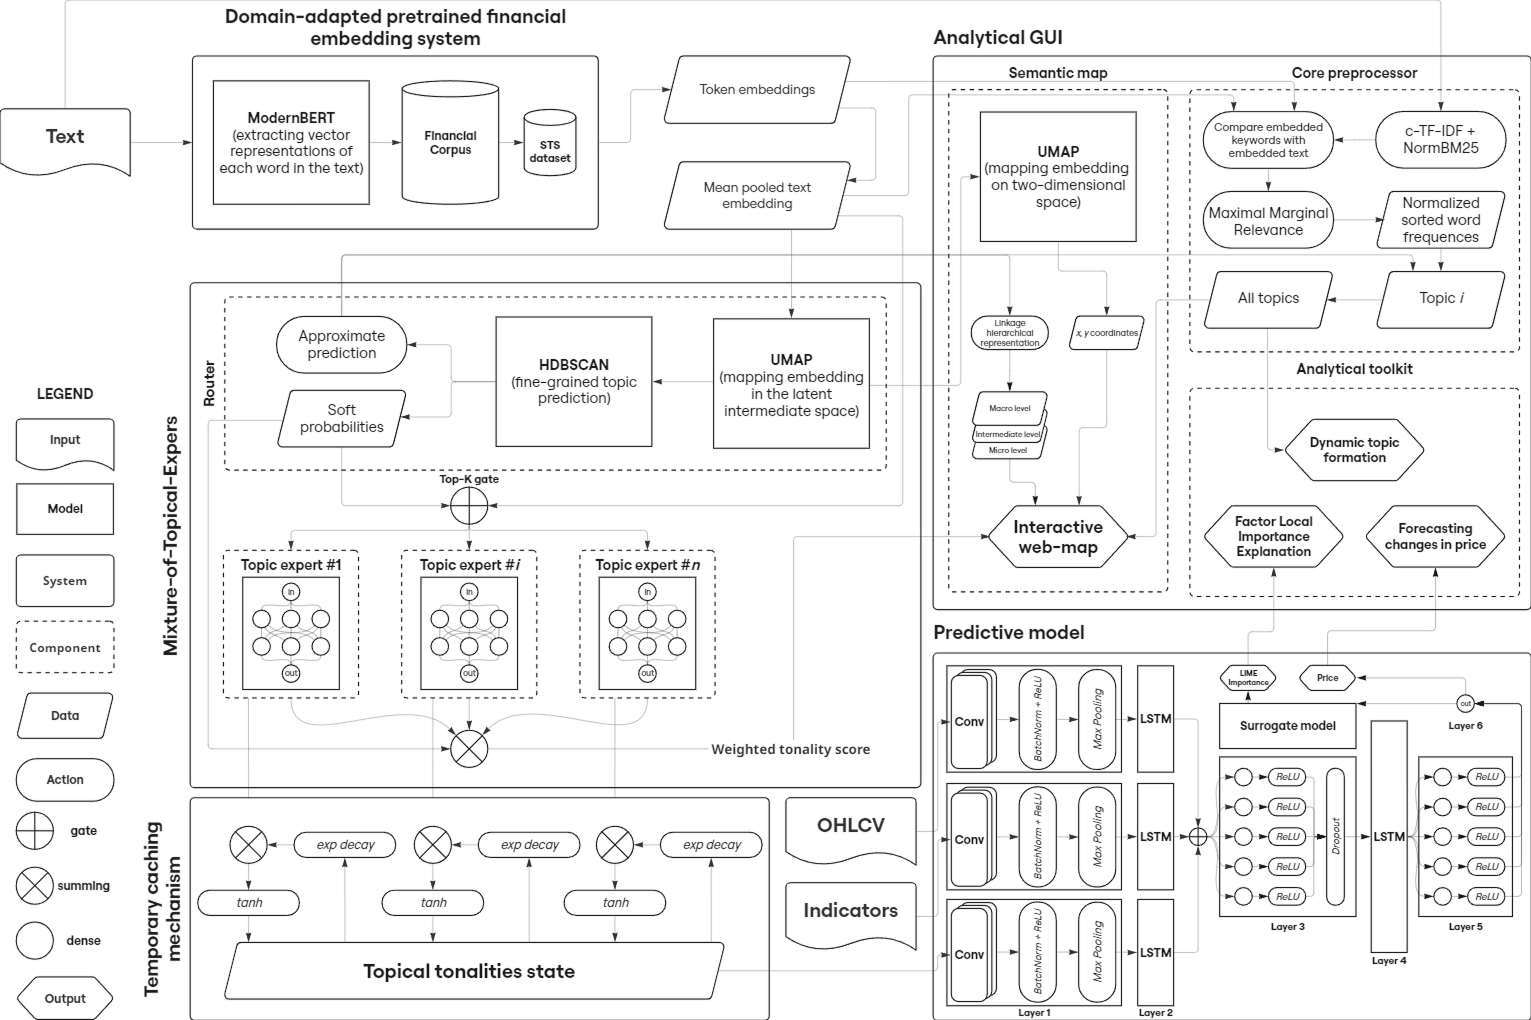
\includegraphics[width=1\linewidth]{img/architecture_overview.png}
    \caption{Обзор спроектированной архитектуры FinABYSS.}
    \label{fig:architecture_overview}
\end{figure}

Спроектированная система состоит из пяти основных модулей (Изображение \ref{fig:architecture_overview}):

\begin{itemize}
    \item Финансовая языковая модель (доменно-адаптированная, тонко настроенная для задачи STS), выдающая векторные представления текста целиком и для каждого токена.
    \item Смесь тематических экспертов (Mixture-of-Topical-Experts, MoTE), формирующая тональность публикации по каждой теме.
    \item TCM, выравнивающий тематические векторы по временным меткам биржевых данных.
    \item Ядровая предиктивная модель с CNN-LSTM и медленным слиянием, обрабатывающая все модальности и предсказывающая цену актива.
    \item Аналитический графический интерфейс (GUI), агрегирующий промежуточные результаты для последующего финансового анализа.
\end{itemize}

Таким образом, созданная архитектура представляет собой мощный и адаптируемый инструмент
для прогнозирования стоимости финансовых активов на основе комплексной оценки тематических сентиментов публикаций.

\subsubsection{Эмбеддинговая система}
Приступая к рассмотрению отдельных блоков разработанной архитектуры, следует начать с этапа предобработки данных.
Наиболее ресурсоёмким и сложным из них является подготовка внебиржевых текстовых источников.

Сразу после поступления в систему текст проходит первичную обработку с помощью доменно‑адаптированной финансовой
эмбеддинговой модели, настроенной на задачу STS. В результате работы этой
модели извлекаются векторные представления для каждого токена, что позволяет сохранить тонкие контекстные связи
внутри предложений. По мере появления новых версий эмбеддинговых моделей важно регулярно обновлять базовую модель
и повторно адаптировать её к специфике финансового домена.

Простейший путь доменной адаптации включает дополнительную стадию обучения на задаче MLM. В качестве корпуса
для этой цели может использоваться корпус финансовых публикаций, сформированный в ходе настоящего исследования,
либо его расширенная версия, а также другие релевантные текстовые корпусы. Для тонкой настройки под задачу STS
иногда применяют небольшие размеченные датасеты, однако для экономии ресурсов возможно обойтись и без них,
используя методы контрастивного обучения на случайных подвыборках основного корпуса \parencite{gao2021simcse}.

После извлечения эмбеддингов токенов производится их агрегирование: обычно применяется усреднение, что даёт векторное
представление всего документа. Далее документ и его эмбеддинги (как токенов, так и усреднённый вектор) передаются
в аналитический модуль для визуализации и интерпретации результатов. Параллельно вектор документа направляется
в блок MoTE, где на его основе формируются тематические тональности публикации.

В качестве конкретной реализации в данном исследовании используется модель 'gte-modernbert-base', построенная на архитектуре
ModernBERT. Несмотря на то, что изначально она не проходила доменную адаптацию, она демонстрирует высокую эффективность:
при кластеризации эмбеддингов удалось получить DBCV-индекс 0.407, а визуальный и контекстуальный анализ показали чёткое разделение тематических групп.

Таким образом, предложенный этап предобработки обеспечивает:

\begin{itemize}
    \item Сохранение глубоких семантических связей на уровне токенов и всего документа.
    \item Гибкость и воспроизводимость процесса адаптации модели к финансовому корпусу.
    \item Интеграцию результатов в соседние блоки архитектуры --- MoTE и аналитический GUI.
\end{itemize}

\subsubsection{Смесь тематических экспертов}

Данный блок использует современную архитектуру Mixture-of-Experts (MoE), успешно применяемую в крупных
языковых моделях (например, Mixtral 8×7B, DeepSeek R1) и в исследованиях Google (Switch Transformer) \parencite{fedus2022switch}.
Основные компоненты данного блока --- обучаемый роутер и множество экспертов --- позволяют динамически активировать
лишь небольшую часть параметров при инференсе, обеспечивая высокую пропускную способность и эффективность
\parencite{shazeer2017outrageously}. Специально для анализа финансовых текстов эксперты тематически
специализированы, что повышает интерпретируемость и точность оценки тональности публикаций.

Архитектура MoE построена на принципе условных вычислений: лишь часть подсетей («экспертов») активна
для каждого входного примера, что снижает вычислительные затраты при огромном общем числе параметров
\parencite{shazeer2017outrageously}.


\begin{itemize}
    \item Роутер получает на вход эмбеддинг документа и вычисляет распределение «весов» для всех экспертов,
    после чего выбирает либо топ-K экспертов, либо тех, чей вес превышает заданный порог, являющийся гиперпараметром.
    \parencite{fedus2022switch}.
    \item Эксперты представляют собой неглубокие feed-forward сети, каждая из которых специализируется на своей
    тематике (в контексте работы --- на одной из финансовых тем) \parencite{shazeer2017outrageously}.
\end{itemize}

При обработке каждого эмбеддинга активизируется лишь малая часть экспертов --- обычно по Top $K$
(выбор $K$ наиболее релевантных экспертов) или по пороговому значению (вес эксперта выше заданного порога) ---
что делает MoE чрезвычайно экономным с точки зрения вычислений при колоссальном общем числе параметров \parencite{fedus2022switch}.
Значения $K$ и $\theta$ выступают гиперпараметрами и настраиваются на валидационных данных.

Для анализа финансовых текстов MoE-модель является логичным выбором, поскольку публикации часто содержат смесь
смежных тематик (макроэкономика, корпоративные отчёты, геополитика и др.), и требуется оценить тональность
под разными углами. Эксперты позволяют формировать специализированные оценки по каждой теме одновременно,
сохраняя «чистоту» низкоуровневой обработки и обеспечивая интерпретируемость результатов \parencite{jacobs1991adaptive}.
Тем не менее, стоит отметить и высокую сложность подбора $K$ или $\theta$ гиперпараметров \parencite{jacobs1991adaptive}.

Вместо обучения экспертов на субъективно размеченных данных их параметры оптимизируются обратным распространением ошибки,
поступающей из блока предсказания цен активов. Это гарантирует, что каждый эксперт обучается напрямую на влиянии публикаций
на стоимость активов, а не на внешних аннотациях \parencite{shazeer2017outrageously}. После получения тематических тональностей
они агрегируются взвешенным суммированием с учётом вероятностей тем, нормализуются и направляются в аналитическую
систему для визуализации, а также в механизм кэширования признаков для синхронизации с биржевыми данными.

Таким образом, блок MoTE на базе MoE обеспечивает обеспечивает сочетание масштабируемости,
эффективности и интерпретируемости при анализе финансовых текстов. Динамическая активация небольшого числа
экспертов позволяет обрабатывать огромные модели без пропорционального роста вычислений, а обучение экспертов через
сигнал от модели прогнозирования цен делает оценку тональностей объективной и близкой к экономической реальности.
Таким образом, предлагаемая архитектура открывает новые возможности для точного прогнозирования и глубокого анализа
влияния текстовых публикаций на стоимость финансовых активов.

\subsubsection{Механизм кэширования признаков}
FCM представляет собой центральный компонент архитектуры, обеспечивающий синхронность между биржевыми данными
(регулярно поступающими временными рядами) и внебиржевыми текстовыми «тиками», разбросанными во времени.
Когда из блока Смеси Тематических Экспертов поступает новая оценка тональности публикации по теме $i$,
она моментально добавляется в матрицу накопительных экспоненциально сглаженных значений по Формуле \ref{eq:exp_decay}:

\begin{equation}\label{eq:exp_decay}
    x_{i,t}=x_{i, t-1} + x_{i, 0} \cdot e^{-\lambda \cdot t},
\end{equation}

где $x_{i, 0}$ --- исходная тональность по теме $i$, $x_{i,t-1}$ --- предыдущее сглаженное значение,
а $\lambda$ --- гиперпараметр скорости экспоненциального «затухания» сигнала. Такой подход отражает
запаздывающую и сглаженную во времени реакцию участников рынка на публикации.

Данный подход учитывает, что реакция участников рынка на информационные события задерживается и распределена
во времени: первая «волна» восприятия быстро затухает, за ней следуют более плавные и длительные эффекты,
что в финансах традиционно моделируется экспоненциальным спадом.

Так как исходные тональности нормированы в диапазоне $[-1,1]$, накопительное суммирование по первой формуле
может выходить за эти границы. Чтобы сохранить скалирование в допустимых интервалах и придать плавность
накоплению, предлагается повторно нормировать результаты с помощью гиперболического тангенса (Формула \ref{eq:tanh1}):

\begin{equation}\label{eq:tanh1}
    tone_{i, t} = \tanh(tone_{i, t-1} + x_{i,t}) =
    \cfrac{
        \tanh{(tone_{i, t-1})} + \tanh{(x_{i,t})}
    }{
        1 + \tanh{(tone_{i, t-1})} \cdot \tanh{(x_{i,t})}
    }.
\end{equation}

что эквивалентно Формуле \ref{eq:tanh2}:

\begin{equation}\label{eq:tanh2}
    tone_{i, t} =
    \cfrac{
        (1-e^{-2 \cdot tone_{i, t}})+(1-e^{-2x_{i,t}} - (1-e^{-2 \cdot tone_{i, t}}) \cdot(1-e^{-2x_{i,t}})
    }{
        (1+e^{-2 \cdot tone_{i, t}})+(1+e^{-2x_{i,t}} - (1+e^{-2 \cdot tone_{i, t}}) \cdot(1+e^{-2x_{i,t}})
    },
\end{equation}

где $tone_{i, t}$ --- текущая нормированная экспоненциально сглаженная тональность по теме $i$ на момент $t$.

В результате непрерывной работы FCM формируется матрица накопительных тематических тональностей,
обновляемая при каждом поступлении текстового «тика». Пока биржевые данные (OHLCV и индикаторы)
отсутствуют, этот временной ряд накапливает сигналы «рыночного сентимента». Как только в систему
приходит новый временной ряд биржевых измерений (с учётом сетевой задержки $\delta$), накопленные
и нормированные тональности конкатенируются с ценовыми и индикаторными данными и передаются
в предиктивную модель для совместной обработки.

Динамический процесс работы механизма проиллюстрирован на Изображении \ref{fig:feature_caching_mechanism}.
Во входной момент кэш инициализируется нулевыми значениями, затем при каждом поступлении текстовой оценки
обновляется по формуле \ref{eq:exp_decay}, после чего нормируется функцией гиперболической тангенсоиды. По достижении триггера ---
момента $t$ или поступления биржевых данных в момент $t+\delta$ --- объединённый временной ряд передаётся дальше.

\begin{figure}[H]
    \centering
    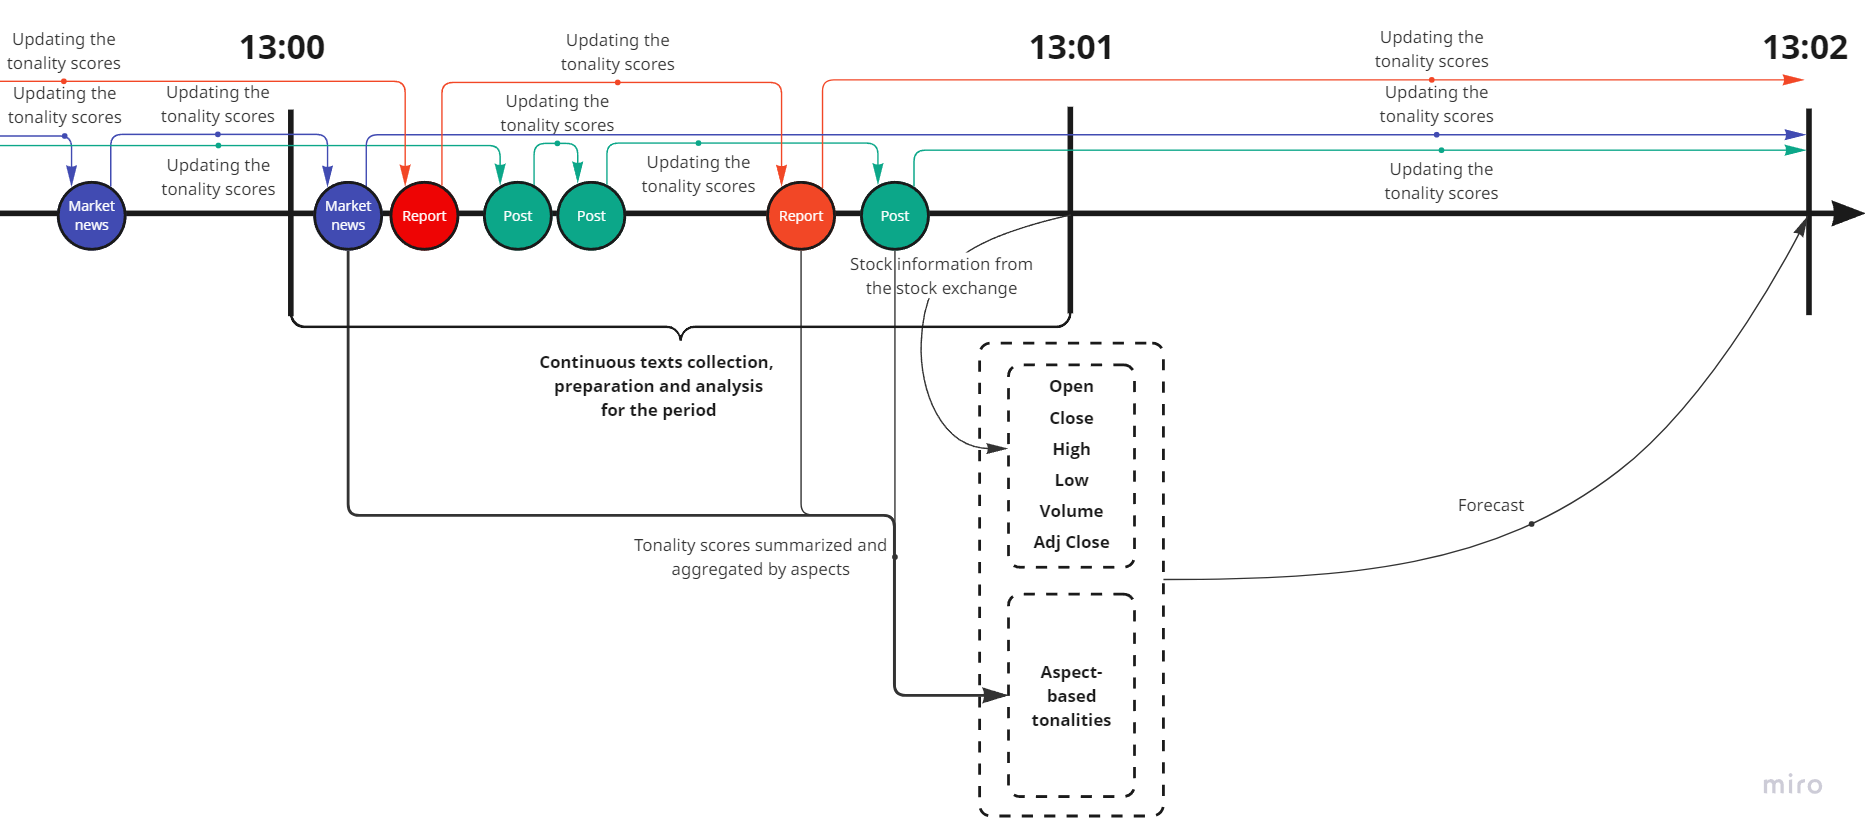
\includegraphics[width=1\linewidth]{img/feature_caching_mechanism.png}
    \caption{Динамическая репрезентация сихронизации внебиржевых данных при помощи FCM на минутном свечевом интервале.}
    \label{fig:feature_caching_mechanism}
\end{figure}

Таким образом, FCM выполняет следующие функции: преобразует нерегулярные текстовые
события в непрерывный многомерный временной ряд, применяет адекватное финансовым реалиям сглаживание и масштабирование
тональностей, а также гарантирует синхронизацию с биржевыми данными. Это обеспечивает согласованность и стабильность
входных признаков в предиктивной модели и способствует повышению точности прогнозирования стоимости финансовых активов.

\subsubsection{Предиктивная модель}
В предлагаемой гибридной архитектуре мы стремимся объединить преимущества свёрточных слоёв для локального
выделения признаков и рекуррентных модулей для моделирования длительных зависимостей, одновременно
обеспечив адаптивное слияние количественных и качественных сигналов. На вход подаётся многомерный
временной ряд длины $T$, в котором каждому временному шагу $t$ соответствует вектор
$x_t = [x_t^{\rm price}, x_t^{\rm ind}, x_t^{\rm sent}]$, где $x_t^{\rm price}\in\mathbb{R}^{C_p}$
содержит OHLCV, $x_t^{\rm ind}\in\mathbb{R}^{C_i}$, а $x_t^{\rm sent}\in\mathbb{R}^{C_s}$ ---
набор скользящих и сглаженных значений тональностей новостей.

Сначала данные разбиваются на три ветви: «Price», «Indicator» и «Sentiment». Каждая ветвь проходит два
базовых уровня обработки. На первом уровне в каждой ветви последовательность $\{x_t^{(\cdot)}\}_{t=1}^T$
пропускается через одномерную свёртку с небольшими ядрами и операциями пулинга (Формула \ref{eq:relu_pooling})

\begin{equation}\label{eq:relu_pooling}
    y^{(\ell+1)}_{t} = \mathrm{ReLU}\bigl(W^{(\ell)} * y^{(\ell)}_{t} + b^{(\ell)}\bigr), \\
    y^{(\ell+\tfrac12)}_{t} = \max\bigl(y^{(\ell+1)}{t},\,y^{(\ell+1)}_{t+1}\bigr).
\end{equation}

где символ $*$ обозначает свёртку по времени, функция активации $\mathrm{ReLU}$ определяется следующим образом (Формула \ref{eq:relu}):

\begin{equation}\label{eq:relu}
    \mathrm{ReLU}(x)=\max(0, x).
\end{equation}

Затем операция max пулинга сокращает временную размерность вдвое. Такая последовательность позволяет
в начальных слоях выделить локальные шаблоны внутри каждого потока, будь то короткие ценовые колебания,
импульсы индикаторов или флуктуации сентимента.

Далее на выходе пулинга в каждой ветви обучается рекуррентный модуль LSTM, который моделирует накопление
и забывание информации с учётом длительных временных зависимостей. Пусть $h_t$ и $c_t$ — скрытое состояние
и ячейка памяти LSTM; их эволюция задаётся стандартными уравнениями входных-, забывающих- и выходных-гейтов. Благодаря
этому каждая ветвь самостоятельно учится определять, какие локальные признаки значимы для прогнозирования
на более отдалённых временных горизонтах.

После того как каждая ветвь выдала своё скрытое состояние $h_t^{\mathrm{price}}$, $h_t^{\mathrm{ind}}$, $h_t^{\mathrm{sent}}$
на каждом временном шаге, происходит этап адаптивного слияния. Для этого векторная конкатенация $u_t$ пропускается через
гейтовый слой (Формула \ref{eq:gate})

\begin{equation}\label{eq:gate}
    g_t = \sigma\bigl(W_g\,u_t + b_g\bigr).
\end{equation}

где $\sigma$ --- сигмоида и $g_t\in(0,1)^{\dim u}$ задаёт поэлементные коэффициенты,
контролирующие относительный вклад каждого потока. Само же объединённое представление вычисляется как

\begin{equation}
    m_t = g_t\odot u_t + (1-g_t)\odot\mu(u_t).
\end{equation}

где $\mu(u_t)$ может быть усреднением или другим агрегатором компонентов вектора $u_t$.
Такой механизм позволяет модели динамически переключаться между акцентом на ценовых паттернах,
индикаторных сигналах или сентименте в зависимости от контекста конкретного временного отрезка.

Объединённая последовательность $\{m_t\}_{t=1}^{T/2}$ затем вновь поступает в рекуррентный модуль
LSTM, который, подобно предыдущим, аккумулирует информацию о совместном развитии трёх модальностей
на более высоком уровне абстракции. Его выходом служит последнее скрытое состояние
$h_{T/2}^{\mathrm{merge}}$, содержащее сжатое резюме всей истории. Для придания нелинейности
и дополнительного измерения выразительности это состояние может быть пропущено через полносвязный
слой с функцией $\mathrm{ReLU}$, а затем — через слой Dropout для регуляризации и смягчения переобучения.

Наконец, заключительный слой без активации переводит полученный вектор в одномерное предсказание
$\hat y$, которое интерпретируется как новая цена (в режиме регрессии).

Также, стоит отметить, что, в целях, локальной интерпретируемости оценок тональности важную роль
в архитектуре играет наличие отдельной суррогатной модели, которая на основе выборки ряда
тональностей, полученного из Feature Caching Mechanism, с дополнительными волнениями,
оценивает вклад каждой тематической тональности в итоговое предсказание стоимости актива.

Таким образом, предложенная гибридная архитектура объединяет локальную детекцию паттернов
(одномерной свёртки), способность LSTM моделировать длительные зависимости, а также механизм
адаптивного слияния, позволяющий динамически регулировать вклад ценовых, индикаторных и сентиментальных
сигналов. Это обеспечивает высокую точность прогнозов при умеренной вычислительной сложности
и прозрачности модели относительно используемых признаков, при этом оставаясь более лёгкой
и прозрачной по сравнению с трансформерными аналогами.

\subsubsection{Аналитический графический интерфейс}
\label{sec:gui}
В завершение описания архитектуры FinABYSS необходимо остановиться на ключевом пользовательском компоненте ---
Аналитическом GUI. Этот модуль аккумулирует результаты всех предыдущих этапов:
от предобработки внебиржевых текстов и их тематической интерпретации в блоке MoTE до конкатенации
с ценовыми и индикаторными рядами в предиктивной модели. На вход GUI поступают промежуточные и финальные данные,
а его задача --- привести их в наглядный, интерактивный и аналитически релевантный вид. GUI состоит
из трёх взаимосвязанных компонент, реализующих постобработку данных, предоставление инструментов
глубокого анализа и визуализацию семантических связей между документами.

Первый компонент --- ядровой постпроцессор --- отвечает за трансформацию «сырых» выходов предыдущих
блоков в упорядоченные и компактные репрезентации. На этапе инициализации он вычисляет относительные
частоты терминов с помощью BM25-модификации TF-IDF и дополнительной нормализации, что удаляет шумовые
и часто встречающиеся, но семантически незначимые токены (например, названия агрегаторов типа Zacks).
Далее, после получения эмбеддингов токенов и всего документа из доменно‑адаптированной языковой модели,
выполняется ранжирование $n$‑грамм по частотам с учётом косинусного сходства между векторами токенов
и документного вектора. Для обеспечения баланса между релевантностью и диверсификацией подсистемы
применяется алгоритм MMR: при разбиении на биграммы MMR устраняет дублирующиеся или избыточно близкие
по смыслу фрагменты, оставляя наиболее информативные. Например, из сырых биграмм «ai» и «ai stocks»
в зависимости от относительной частоты и семантической близости могут сохраниться либо «ai» и «stocks»,
либо только «ai stocks», либо только «ai», что повышает однородность итогового словаря и уменьшает
избыточность.

После применения MMR словарь сортируется по итоговым частотам, и постпроцессор получает от блока MoTE метку
кластера, к которому принадлежит текущий документ. На основе этой кластерной принадлежности осуществляется
инкрементальное обновление c‑TF‑IDF статистики: накопленные частоты слов внутри каждого кластера корректируются
с учётом новой публикации, что обеспечивает адаптивность и учёт эволюции тематических трендов во времени
и используется для динамического тематического моделирования. Параллельно от постпроцессора поступают два
потока данных: обогащённые частотные признаки и другие извлечённые метаданные текста направляются
в аналитический инструментарий, а сам очищенный и классифицированный текст с эмбеддингами --- в Семантическую карту.

Второй компонент --- Аналитический инструментарий --- представляет собой набор визуальных и интерактивных элементов,
позволяющих пользователю углублённо исследовать динамику тематических трендов и их влияние на цены активов.
Через дашборды можно получать:

\begin{itemize}
    \item исторические графики тональностей по каждой теме, совмещённые с ценовыми рядами и техническими индикаторами;
    \item динамические корреляционные матрицы между темами и движениями цен;
    \item сводные отчёты по влиянию макро‑, мезо‑ и микротем на волатильность и трендовые движения;
    \item агрегированные показатели рыночной тональности (взвешенная суммарная тональность по всем темам) с трендовыми линиями.
\end{itemize}

Инструментарий разработан с учётом будущего расширения: при добавлении новых модальностей
(изображения, графовые данные, аудио‑ или видеопотоки) к нему легко интегрируются модальностно‑специфичные
виджеты --- например, интерактивные облака ключевых сущностей, графы взаимосвязей эмитентов
или тепловые карты тональностей в голосовых и видео‑форматах.

Третий компонент --- Семантическая карта --- реализует двумерную визуализацию эмбеддингов документов.
На основе заранее обученной модели понижения размерности каждое документное представление из латентного
пространства, где проводилась кластеризация, отображается в координатах $(x,y)$. Параллельно используется
аппроксимальный предсказатель темы из блока Смеси Тематический Экспертов: по каждому документу
определяется иерархически организованная тройка тематических меток --- на макро‑, мезо‑ и микроверсиях.
Цвет, размер и форма маркеров на карте кодируют принадлежность к кластеру, силу тональности и объём
текста. Это позволяет анализировать не только пространственное соседство публикаций, но и их тематическую
многоуровневую структуру, быстро выявлять периферийные и центральные документы, а также отслеживать
эволюцию тематических сообществ.

В совокупности GUI создаёт единую интерактивную панораму, в которой результаты глубочайших вычислительных блоков
--- от FCM и MoTE до гибридной CNN-LSTM предиктивной модели — превращаются в интуитивно понятный и аналитически
ёмкий инструмент. Пользователь получает возможность не просто просматривать прогнозы цен, но и детально исследовать
причинно‑следственные связи между медиасигналом и движением рынка.

Аналитический графический интерфейс FinABYSS обеспечивает сквозную визуализацию и интерпретацию выходных данных
системы, интегрируя частотные, тематические и эмбеддинговые признаки в три взаимосвязанных подсистемы. Ядровой
постпроцессор трансформирует «сырые» текстовые и числовые данные в компактные и репрезентативные признаки,
аналитический инструментарий предлагает гибкие средства глубокого исследования влияния тем на стоимость активов,
а семантическая карта даёт наглядное отображение многомерных эмбеддингов с учётом иерархической тематики.
Благодаря такому сочетанию технологической мощности и удобства взаимодействия GUI выступает завершающим,
но не менее важным звеном в конвейере прогнозирования, обеспечивая прозрачность, адаптивность и наглядность
результатов для экспертов в области финансов.


\subsection{Finished System Components}
\subsubsection{Эмбеддинговая система и роутер}
\label{sec:emb_sys_and_router}

Основным итогом настоящего исследования стало создание двух ключевых компонентов: гибкой эмбеддинговой подсистемы
и обучаемого роутера для блока MoTE. Эти наработки не только обеспечивают надёжный фундамент для дальнейшего
развития FinABYSS, но и открывают широкий простор для применения в смежных прикладных проектах.

В рамках исследования мы провели серию экспериментов по отбору оптимальных комбинаций эмбеддинговых моделей,
методов понижения размерности и алгоритмов кластеризации, используя разные метрики для настройки гиперпараметров.
На первом этапе базовая цепочка состояла из ModernBERT, UMAP (косинусная метрика), HDBSCAN (эвклидова метрика)
оптимизировалась по коэффициенту силуэта. Несмотря на удовлетворительные результаты, мы отметили сильную
зависимость от структуры кластеров и чувствительность силуэта к форме кластеров.

Второй этап повторил ту же связку, но в качестве целевой метрики был выбран DBCV-индекс. Благодаря свойству
DBCV учитывать плотностные особенности и неоднородность распределения точек, гиперпараметры, подобранные
под DBCV, обеспечили более семантически согласованные и плотные кластеры.

Наконец, мы протестировали тонко настроенную на задачу STS версию ModernBERT ('gte-modernbert-base') \parencite{Warner2024ModernBERT, MGTE2024} в сочетании с UMAP,
но уже с $L_2$–эвклидовой метрикой, и тем же HDBSCAN, так же использующим $L_2$–евклидову метрику для вычисления меры дистанции (Таблица \ref{tab:experiment_configs}).
Однако это сочетание уступило предыдущему: полученный DBCV-индекс составил лишь 0.397 против 0.407 у пары косинусной с евклидовой метрикой рассояния (Таблица \ref{tab:experiment_results}).

\begin{longtable}[c]{|l|ll|}
    \caption{Description of the final configurations of experiments conducted on a subsample of 10,000 embeddings.}
    \label{tab:experiment_configs}\\
    \hline
    \multicolumn{1}{|c|}{\multirow{2}{*}{\textbf{Model}}} & \multicolumn{2}{c|}{\textbf{Configuration}}                         \\ \cline{2-3}
    \multicolumn{1}{|c|}{}                                 & \multicolumn{1}{c|}{(I)}               & \multicolumn{1}{c|}{(II)}  \\ \hline
    \endfirsthead

    \endhead

    UMAP    & \multicolumn{1}{l|}{$L_2$-Euclidean} & \multicolumn{1}{l|}{Cosine}    \\
    HDBSCAN & \multicolumn{1}{l|}{$L_2$-Euclidean} & \multicolumn{1}{l|}{Euclidean} \\ \hline
\end{longtable}

Дополнительный анализ шумовых точек и структуры кластеров не подтвердил это преимущество (Таблица \ref{tab:experiment_results}),
однако в ходе анализа выяснилось, что подобная ситуация просиъодит по причине внутренней нестрабильности GPU реализации \parencite{cuml2020machine}. На метрике же,
данный факт не сказался существенно негативным образом. При использовании $L_2$–метрики
доля шумовых точек достигала 39.54\%, число кластеров --- 73 (при максимальном размере 3 824 точек и минимальном --- 365).
Для пары "cosine + euclidean" больше точек было отмечено как шум 43.38\%, а число кластеров увеличилось до 141; при этом максимальный
кластер вырос до 2 558 точек, а минимальный сократился до 147. Так как целевая метрика именно DBCV, можно сделать вывод, что
подход "cosine + euclidean" продемонстрировал лучшую устойчивость кластеров.

% Please add the following required packages to your document preamble:
% \usepackage{multirow}
% \usepackage{longtable}
\begin{table}[!htbp]
\begin{longtable}[c]{|cl|cc|}
    \caption{Summary table of the results of hyperparameter optimization performed for three specified configurations on a subsample of 10,000 embeddings.}
    \label{tab:experiment_results}\\
    \hline
    \multicolumn{2}{|c|}{\multirow{2}{*}{\textbf{Best trial}}} & \multicolumn{2}{c|}{\textbf{Configuration}}                                                \\ \cline{3-4}
    \multicolumn{2}{|c|}{}                                     & \multicolumn{1}{c|}{(I)} & \multicolumn{1}{c|}{(II)} \\ \hline
    \endfirsthead

    \endhead

    \hline
    \endfoot

    \endlastfoot

    \multicolumn{1}{|c|}{\multirow{7}{*}{\textbf{Hyperparameters}}} & n\_components            & \multicolumn{1}{c|}{47}                & \multicolumn{1}{c|}{41}             \\
    \multicolumn{1}{|c|}{}                                          & n\_neighbors             & \multicolumn{1}{c|}{70}                & \multicolumn{1}{c|}{75}             \\
    \multicolumn{1}{|c|}{}                                          & min\_dist                & \multicolumn{1}{c|}{0,0}               & \multicolumn{1}{c|}{0,065}          \\
    \multicolumn{1}{|c|}{}                                          & spread                   & \multicolumn{1}{c|}{6,5}               & \multicolumn{1}{c|}{6,4}            \\
    \multicolumn{1}{|c|}{}                                          & negative\_sample\_rate   & \multicolumn{1}{c|}{10}                & \multicolumn{1}{c|}{11}             \\
    \multicolumn{1}{|c|}{}                                          & min\_cluster\_size       & \multicolumn{1}{c|}{360}               & \multicolumn{1}{c|}{145}            \\
    \multicolumn{1}{|c|}{}                                          & min\_samples             & \multicolumn{1}{c|}{180}               & \multicolumn{1}{c|}{170}            \\ \hline
    \multicolumn{1}{|c|}{\multirow{5}{*}{\textbf{Statistics}}}      & Max cluster size         & \multicolumn{1}{c|}{3824}              & \multicolumn{1}{c|}{2558}           \\
    \multicolumn{1}{|c|}{}                                          & Min cluster size         & \multicolumn{1}{c|}{365}               & \multicolumn{1}{c|}{147}            \\
    \multicolumn{1}{|c|}{}                                          & Total clusters           & \multicolumn{1}{c|}{73}                & \multicolumn{1}{c|}{141}            \\
    \multicolumn{1}{|c|}{}                                          & Noise \%                 & \multicolumn{1}{c|}{\textbf{39,54\%}}  & \multicolumn{1}{c|}{43,38\%}        \\
    \multicolumn{1}{|c|}{}                                          & DBCV Index               & \multicolumn{1}{c|}{0,397}             & \multicolumn{1}{c|}{\textbf{0,407}} \\ \hline
\end{longtable}
\end{table}

Экспериментальные результаты однозначно свидетельствуют о превосходстве схемы ModernBERT + UMAP
с косинусной метрикой и HDBSCAN с эвклидовой дистанцией в задачах тематической кластеризации
финансовых текстов. В сочетании с оптимизацией по DBCV-индексу данный подход формирует наиболее
семантически связные группы, минимизирует долю шумовых экземпляров и предоставляет более стабильную
основу для последующего обучения роутера MoTE.

Тем не менее, к сожалению, были выявлены и явные проблемные места текущей реализации.
Полученные кластеры и их структура не могут инкрементально обновляться при потоковых
поступлениях новых публикаций, что происходит по нескольким причинам. Во-первых, обученная
модель является GPU-реализацией из библиотеке 'cuML', в которой лишь после проведения исследования
были обнаружены критические ошибки в коде версии 25.02 \parencite{cuml2020machine}. Во-вторых, выбранный
алгоритм UMAP достаточно плохо работает в инкрементальном режиме по своей природе, именно
поэтому существуют другие реализации, как например AlignedUMAP \parencite{mcinnes2018umap-software}
или ParametricUMAP, основанный на нейронной сети в качестве базовой модели \parencite{ParametricUMAP2020}.
К сожалению, обе данные реализации доступны исключительно для обучения на центральном, а не графическом процессоре.
А для обучения на центральном процессоре в контексте текущего исследования недостаточно вычислительных ресурсов.

Таким образом, узким местом данного исследования и предложенного решения является недостаток вычислительных
мощностей для обучения моделей, что будет доработано в дальнейших исследованиях.

\subsubsection{Семантическая карта}

Наконец, на базе разработанной эмбеддинговой подсистемы и роутера MoTE была обучена отдельная модель UMAP,
призванная переводить векторы из промежуточного латентного пространства кластеризации в двумерное представление,
удобное для визуального анализа. Именно эта проекция лежит в основе Семантической карты финансовых публикаций ---
одного из ключевых компонентов интерфейса FinABYSS, обеспечивающего глубокое и интуитивно понятное исследование
тематической структуры новостных потоков.

\begin{figure}[H]
    \centering
    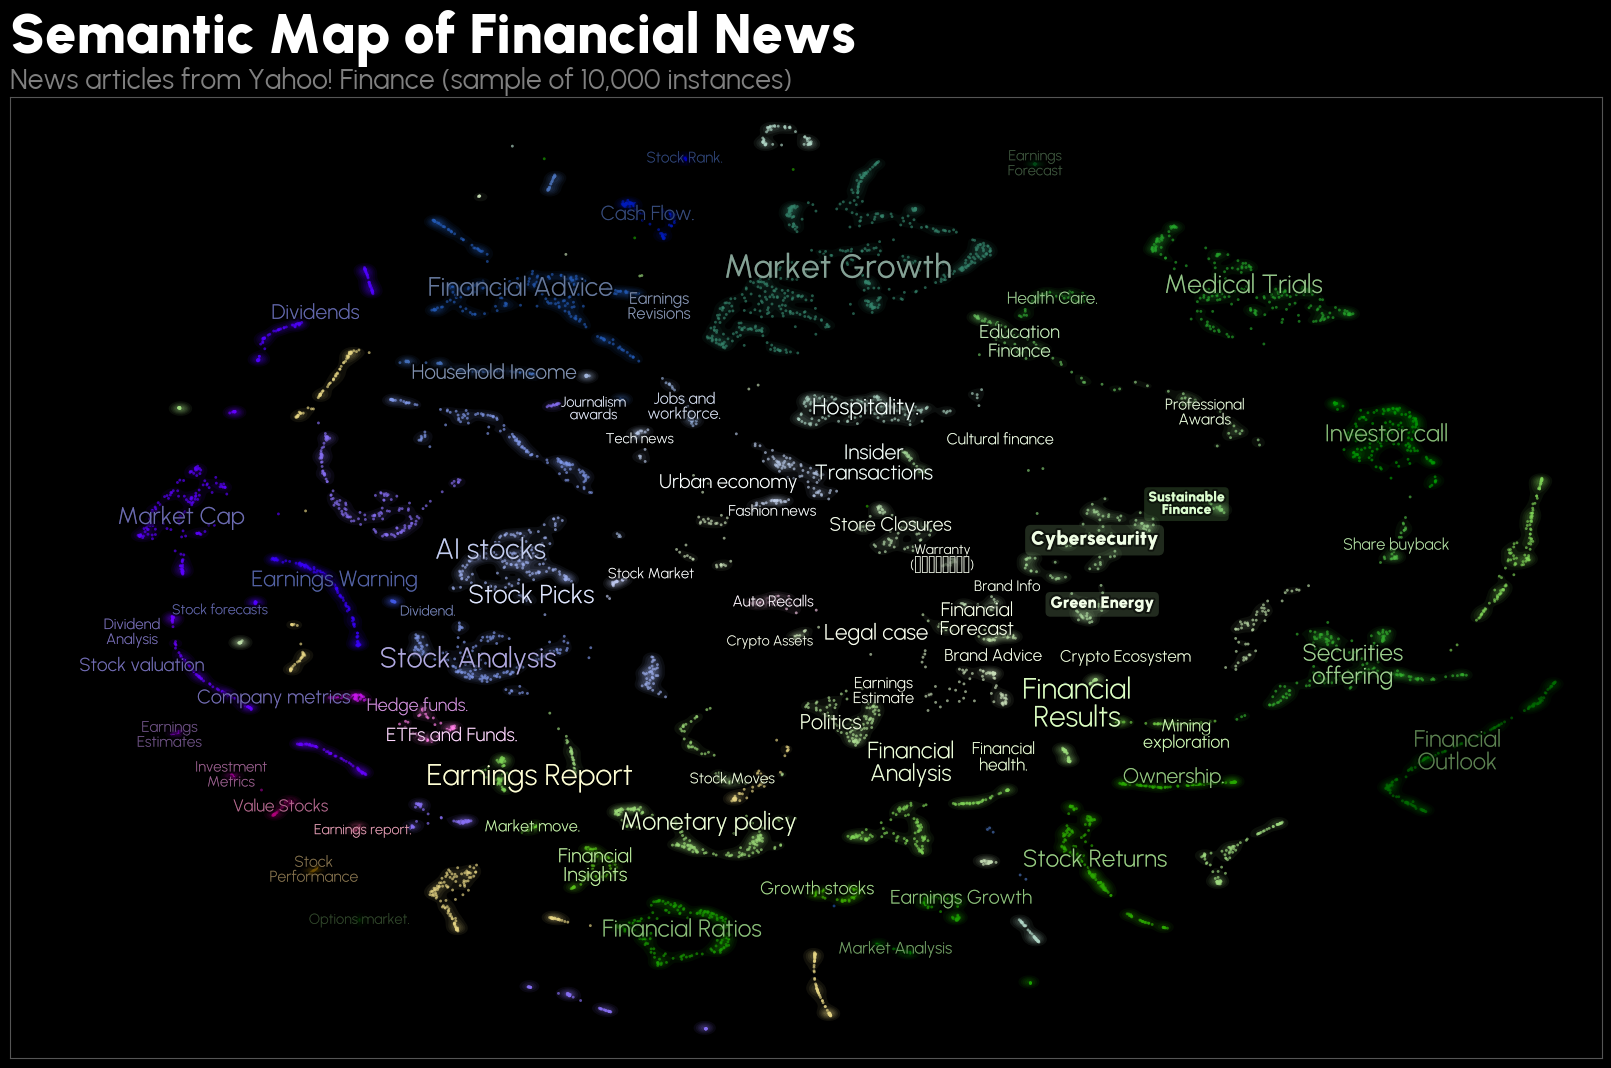
\includegraphics[width=1\linewidth]{img/semantic_map.png}
    \caption{Статичная семантическая карта, разработанная на основе подвыборки из 10 000 финансовых публикаций,
    опубликованных в период с 17.09.2023 по 18.04.2025, и кластеризованных по темам.}
    \label{fig:semantic_map}
\end{figure}

Для начала была реализована статическая версия карты, на которой отображены 100 000 финансовых статей за период
с сентября 2023 по март 2025 года, разбитые на кластеры по тематике (Изображение \ref{fig:semantic_map}).
Каждый кластер промаркирован автоматически сгенерированным словом-меткой без какой-либо ручной аннотации.
Несмотря на автоматический характер присвоения, метки получились репрезентативными: плотные группы статей,
посвящённые здравоохранению, «Устойчивым финансам», «Кибербезопасности» и «Зелёной энергетике», расположены
рядом, что отражает их семантическую близость; аналогично происходит с кластерами «Политика» и «Монетарная политика».

Однако статическая карта демонстрирует потенциал лишь UMAP-проекции. Интерактивная Семантическая
карта FinABYSS выходит далеко за рамки простой визуализации точек:

\begin{itemize}
    \item Наведение курсора на любую точку раскрывает метаданные статьи: заголовок, дата и время публикации,
    иерархическую тему (макро–/мезо–/микротема), автора и источник. При этом доступен предпросмотр полного
    текста и прямая ссылка на оригинал публикации.
    \item Механизм поиска по ключевым словам позволяет быстро отфильтровать статьи, содержащие специальные термины.
    Поиск можно комбинировать с фильтрами по диапазону дат, объёму публикаций и другим числовым признакам (например,
    объёму текста или количеству просмотров), что облегчает точечное обнаружение исторических событий и триггеров
    на графике.
    \item Раздел источники и темы даёт возможность включать и исключать источники новостей или целевые кластеры,
    помогая сфокусироваться на релевантных публикациях в сложных аналитических сценариях.
    \item Также для статей доступна функция облака слов, формируемого на основе наиболее частых слов, встречающихся
    в выделанной группе текстов. Облако слов мгновенно отображает доминирующие термины и паттерны обсуждения,
    что дополняет количественную канву графика качественными характеристиками.
\end{itemize}

Таким образом, Семантическая карта FinABYSS представляет собой полноценную аналитическую систему,
объединяющую мощь выбранных моделей UMAP и HDBSCAN, а при дальнейшем развитии и гибридной CNN-LSTM-архитектуры
и MoE-подхода к оценке тональностей. Она обеспечивает исследователю возможность не только визуально различать
именованные кластеры и их взаимное расположение, но и глубоко погружаться в содержание каждой публикации,
комбинируя автоматические и ручные методы анализа.

Разработанная интерактивная Семантическая карта выступает естественным продолжением предыдущих модулей FinABYSS.
Все звенья конвейера связаны в единую цепь. Инструмент предлагает пользователю прозрачный, масштабируемый
и гибко настраиваемый интерфейс для семантического исследования финансовых новостей, где каждый элемент ---
от кластерных меток до облака слов — отражает результаты вычислительной логики системы и поддерживает экспертные
решения при анализе рыночных процессов.

\subsubsection{Динамическое тематическое моделирование}

Помимо семантической карты, FinABYSS предоставляет мощный инструментарий для анализа лингвистических
особенностей сформированных тематических групп и динамического темпорального моделирования тем.
Все входящие тексты проходят описанный в \hyperref[sec:sys_dev]{Разделе 2.4} пайплайн постобработки в контексте Аналитического
GUI (см. \hyperref[sec:sys_dev]{Раздел 3.1.6}), где каждому документу присваивается превалирующая тема,
а затем извлекаются и агрегируются соответствующие лексические признаки.

Так, система визуализирует частотное распределение самых релевантных слов в рамках выбранной темы
(Изображение \ref{fig:topics_words_freqs}). Такая лингвистическая панель служит двум целям:

\begin{itemize}
    \item Во-первых, это позволяет после разработки системы в ручном режиме провалидировать качество сформированных
    тем и оценить насколько они уникальны и семантически однородны.
    \item Во-вторых, эта функциональность может быть весьма полезна при первичном знакомстве финансового аналитика
    с системой. Финансовый аналитик, впервые работающий с FinABYSS, мгновенно получает представление о содержании каждой темы без глубокого ознакомления с самими текстами.
\end{itemize}

Именно последний факт послужил причиной включения данной функциональности в набор основных инструменты GUI.

\begin{figure}[H]
    \centering
    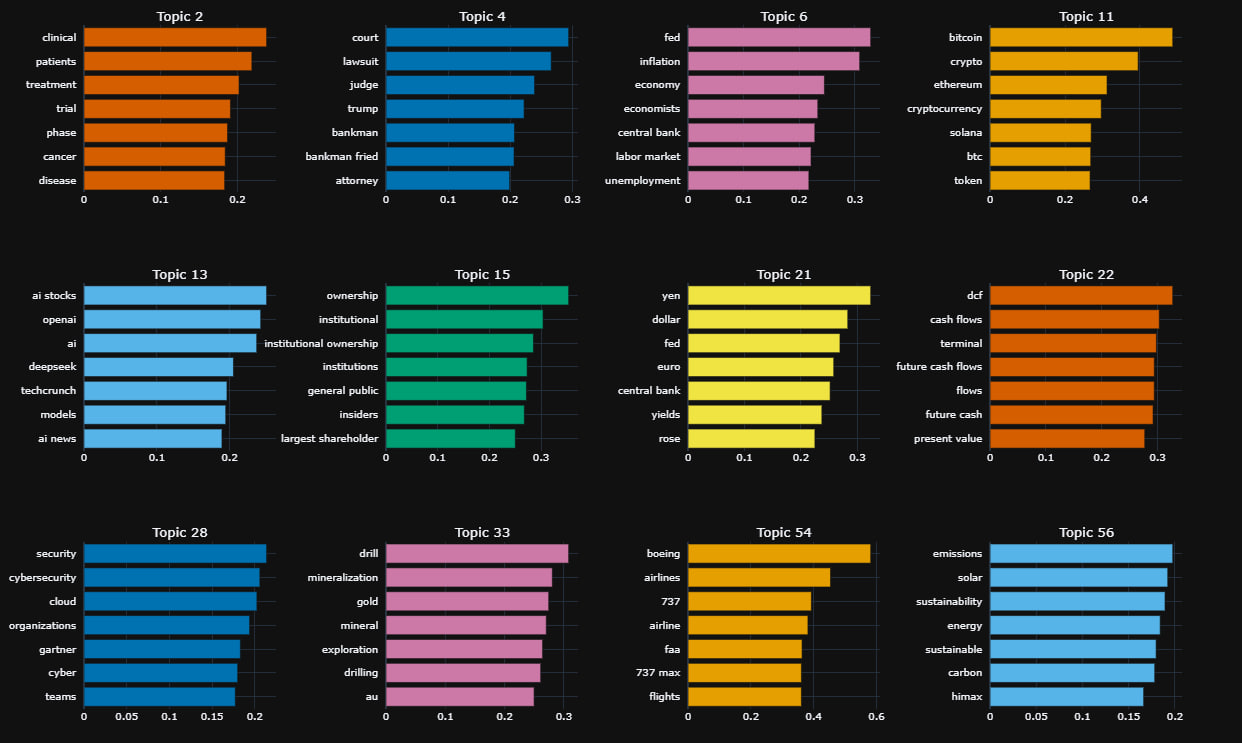
\includegraphics[width=1\linewidth]{img/topics_words_freqs.png}
    \caption{Ранжированные по релевантности термины выборки из 12 тем.}
    \label{fig:topics_words_freqs}
\end{figure}

Для иллюстрации данного функционала случайным образом была сформирована выборка из
125 000 публикаций, внутри которых было выбрано 12 тем для отображения. Среди выборки
все темы несомненно несут прикладное значение для финансовых рынков. Причем есть
более общие отраслевые темы, такие как:

\begin{itemize}
    \item Тема №2, связанная с фармацевтической отраслью;
    \item Тема №13, связанная с сектором искуственного интеллекта;
    \item Тема №28, связанная с кибербезопасностью;
    \item Тема №33, связанная с горнодобывающей отраслью;
    \item Тема №54, связанная с авиационной промышленностью.
\end{itemize}

С другой стороны в выборку попала и достаточно общая тема, которая стоит на повестке дня в том числе и в финансах ---
Тема №56, которая явно относится к ESG. Наконец, есть и узкоспециализированные финансовые темы,
которые также были выявлены автоматически:

\begin{itemize}
    \item Тема №4, связанная с судебными процессами и разбирательствами, потенциально она
    является крайне влиятельной в контексте ценообразования стоимости актива;
    \item Тема №6, связанная с внешнеэкономическими факторами и экономикой, в целом;
    \item Тема №11, напрямую связанная с рынком активов, а именно криптовалют;
    \item Тема №15, связанная с правами собственности, то есть держателями аккий компаний;
    \item Тема №21, связанная с валютным рынком;
    \item Тема №22, связанная с денежными потоками, включая будущие, настоящие и дисконтированные.
\end{itemize}

Так, мы можем наблюдать за лингвистическими особенностями тематических групп,
а также крайне быстро и эффективно изучать как различия между ними, так и конкретные темы вглубь.

С другой стороны, было бы крайне полезно понимать как темы меняются сквозь время, ведь информационное медиапространство
крайне нестабильно, а повестка дня в современном обществе меняется мгновенно. Так, FinABYSS реализует
динамическое тематическое моделирование через интерактивный график тематических временных рядов.

\begin{figure}[H]
    \centering
    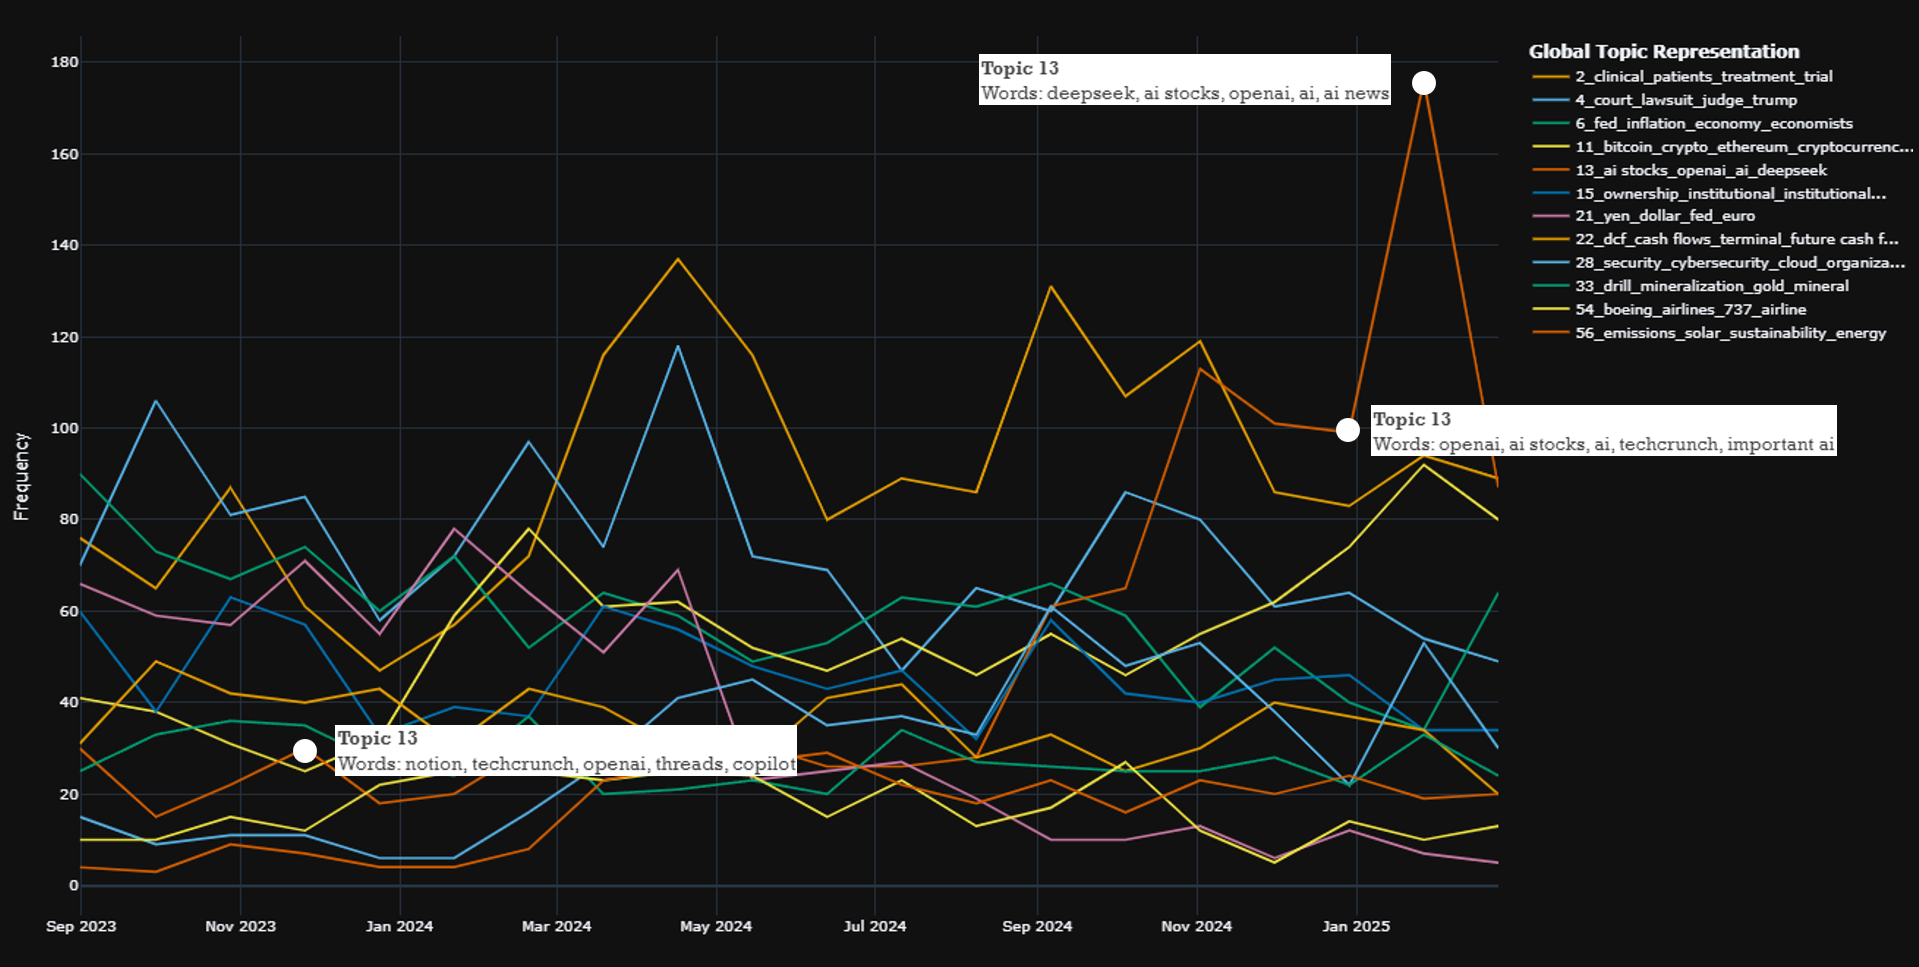
\includegraphics[width=1\linewidth]{img/dynamic_topic_modeling.png}
    \caption{Эволюционное тематическое моделирование и наиболее релевантные термины выборки из 12 тем за период с 17.09.2023 по 18.04.2025.}
    \label{fig:dtm}
\end{figure}

На Изображении \ref{fig:dtm} представлена та же выборка из 12 тем. Ось абсцисс отражает интервал публикаций (настраиваемый:
от дневного до годового), ось ординат --- число статей по каждой теме за соответствующий период. При наведении
курсора выводятся пять наиболее репрезентативных слов, характеризующих тему в данном временном окне. Пользователь может
изменить число отображаемых слов.

Преимущества такого подхода очевидны:

\begin{itemize}
    \item Раннее обнаружение трендов. Аналитик может наблюдать за появлением новых лексических маркеров
    или ростом публикационной активности в тематических группах, что служит сигналом зарождающихся событий.
    \item Отслеживание циклических явлений. Так, для Темы 13 (ИИ) на графике и в декабре 2023 года,
    и в декабре 2024 года появляется слово TechCrunch — название одной из крупнейших и самых престижных
    конференций в сфере IT и AI. Ежегодно конференция выпускает множество крупнейших стартапов, которые
    в дальнейшем получают крупное финансирования. Таким образом, имея данную визуализацию, аналитик может
    меньшими усилиями оставаться в курсе значимых для финансов циклических событий.
    \item Реакция на форс-мажорные события. В феврале 2025 по той же Теме 13 наблюдается резкий пик из-за
    выхода китайской LLM --- DeepSeek R1. Этот инцидент крайне важен, так как в последствии он стал причиной обрушения
    акций Nvidia, крупнейшей компании поставляющей вычислительное оборудование для обучения LLM.
\end{itemize}

Таким образом, FinABYSS не ограничивается статическим построением тематических кластеров:
взаимодействие с лингвистическими метриками и темпоральными трендами превращает систему
в универсальную платформу для финансовой аналитики. Эксперт может переходить от макро-трендов
к микро-лексическим деталям в несколько кликов, комбинировать фильтры по дате, источнику и тематике,
изучать эволюцию терминологии и оперативно реагировать на появление новых ключевых слов или аномальное
изменение релевантности. Это делает FinABYSS не просто инструментом кластеризации, а полноценной экосистемой
для семантического мониторинга рыночных трендов и прогнозирования воздействия медийных сигналов на динамику финансовых
активов.

\subsubsection{Прикладное значение}
\label{sec:practical_importance}

Подводя итоги, стоит подчеркнуть, что разработанная система FinABYSS представляет собой не просто набор моделей,
а полноценный инструмент для оперативного обнаружения критических сигналов на финансовых рынках. Семантическая
карта, глубокая тематическая кластеризация и временные ряды новостей позволяют финансовому аналитику мгновенно
реагировать на неожиданные события, снижать риски и извлекать прибыль.

Так, рассматривая исключительно функциональность Семантической Карты, можно найти несколько критически важных
событий, которые сразу же после попадания в сеть своевременно отразились в тематическом кластере «Судебные
разбирательства».

Так, первый иллюстративный пример (Изображение \ref{fig:citi_group}) демонстрирует, как статья от 22 мая 2024 года
повлияла на стоимость акций целевой компании. Данная новость осветила скандал с обвалом стоимости европейских акций
по причине недостаточного контроля за трейдинговыми операциями со стороны одного из 4 крупнейших банков в мире ---
Citi Group (C.NYSE) — акции которого торгуются на Нью-Йоркской фондовой бирже. После данной новости, которая так же
сообщала о назначении рекордного штрафа банку со стороны британского правительства, за ближайшие 28 часов акции компании
упали почти на 4\%. В последующие 23 дня, пока шли судебные разбирательства, появлялись дополнительные репортажи
и происходила отложенная рыночная реакция, цена уменьшилась почти на 10\%.

\begin{figure}[H]
    \centering
    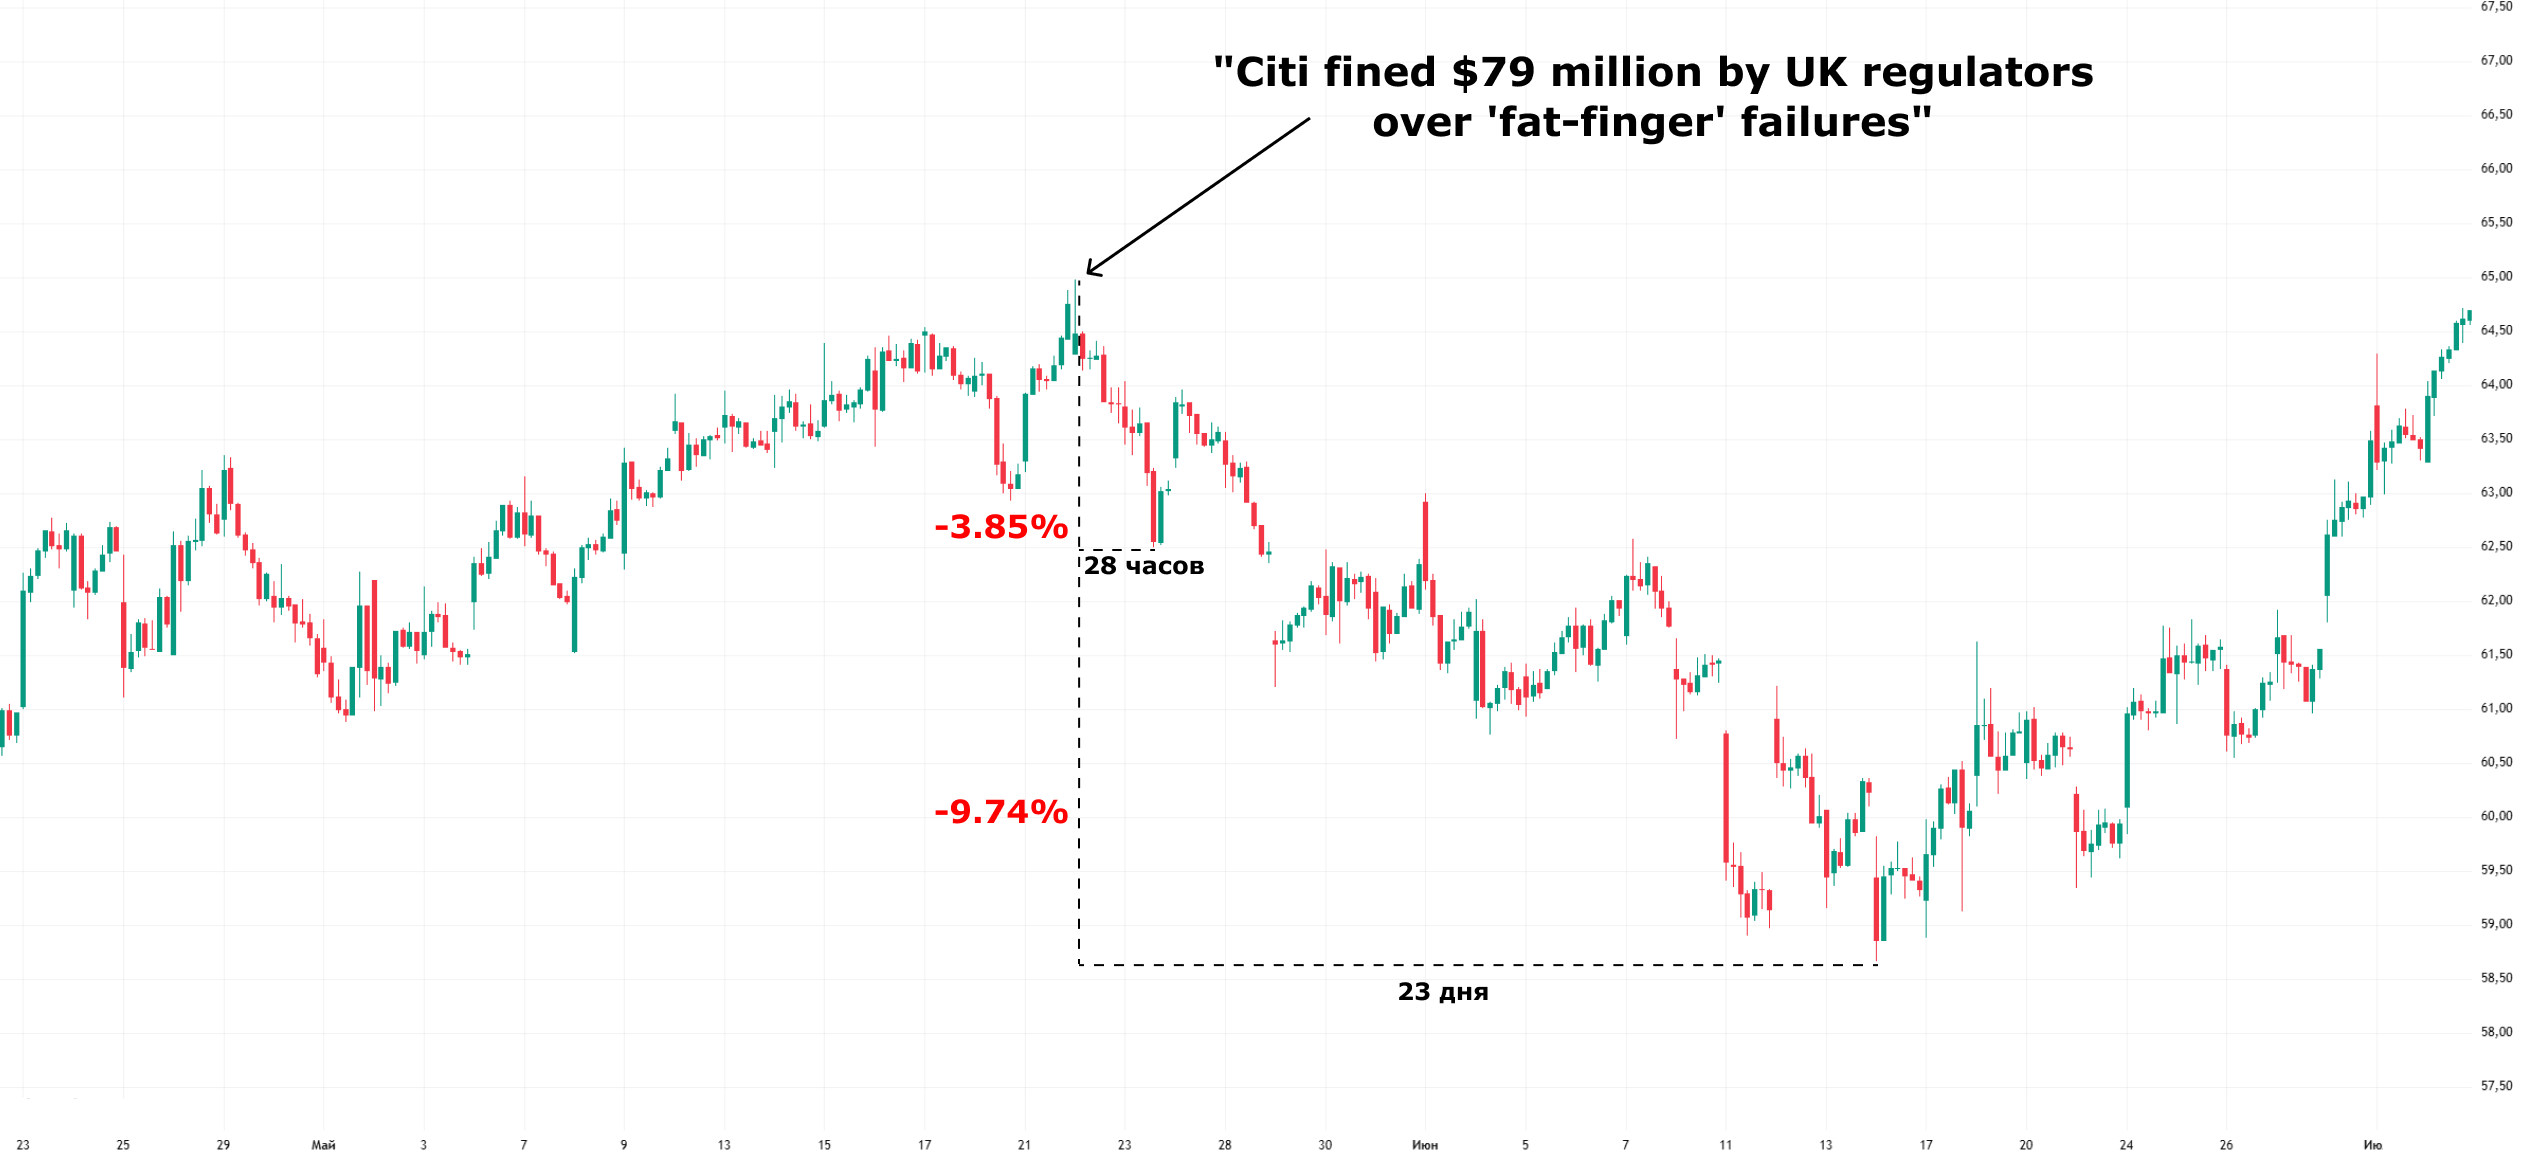
\includegraphics[width=1\linewidth]{img/citi_group.png}
    \caption{Пример падения цены акций одного из крупнейших банков США, Citi Group (C.NYSE),
    из-за обвинений в недостаточном контроле за торговыми операциями, что вызвало падение европейских акций}
    \label{fig:citi_group}
\end{figure}

Сама новостная статья от Reuters послужила сигналом для продажи актива, а на Изображении \ref{fig:citi_group} явно виден
переломный момент с резким падением цены, небольшим откатом и дальнейшей сменой глобального тренда почти на месяц.

Без FinABYSS подобные сигналы часто теряются в потоке новостей, в то время как разработанная система упрощает обнаружение
триггерных событий, посредством реализации возможности отслеживания значимых для конкретного портфеля кластеров.

Второй кейс связан с публикацией от 30 августа 2024 года о возможном отзыве лицензии и штрафе AU\$ 67 млн в отношении крупнейше
 австралийской компании по азартным играм --- The Star Entertainment Group LTD (рис. \ref{fig:star_entertainment}). Новость сообщала
 об обвинениях  в отмывании денег. Акции оказались заморожены на месяц, а при возобновлении торгов их стоимость рухнула на 55\%.

\begin{figure}[H]
    \centering
    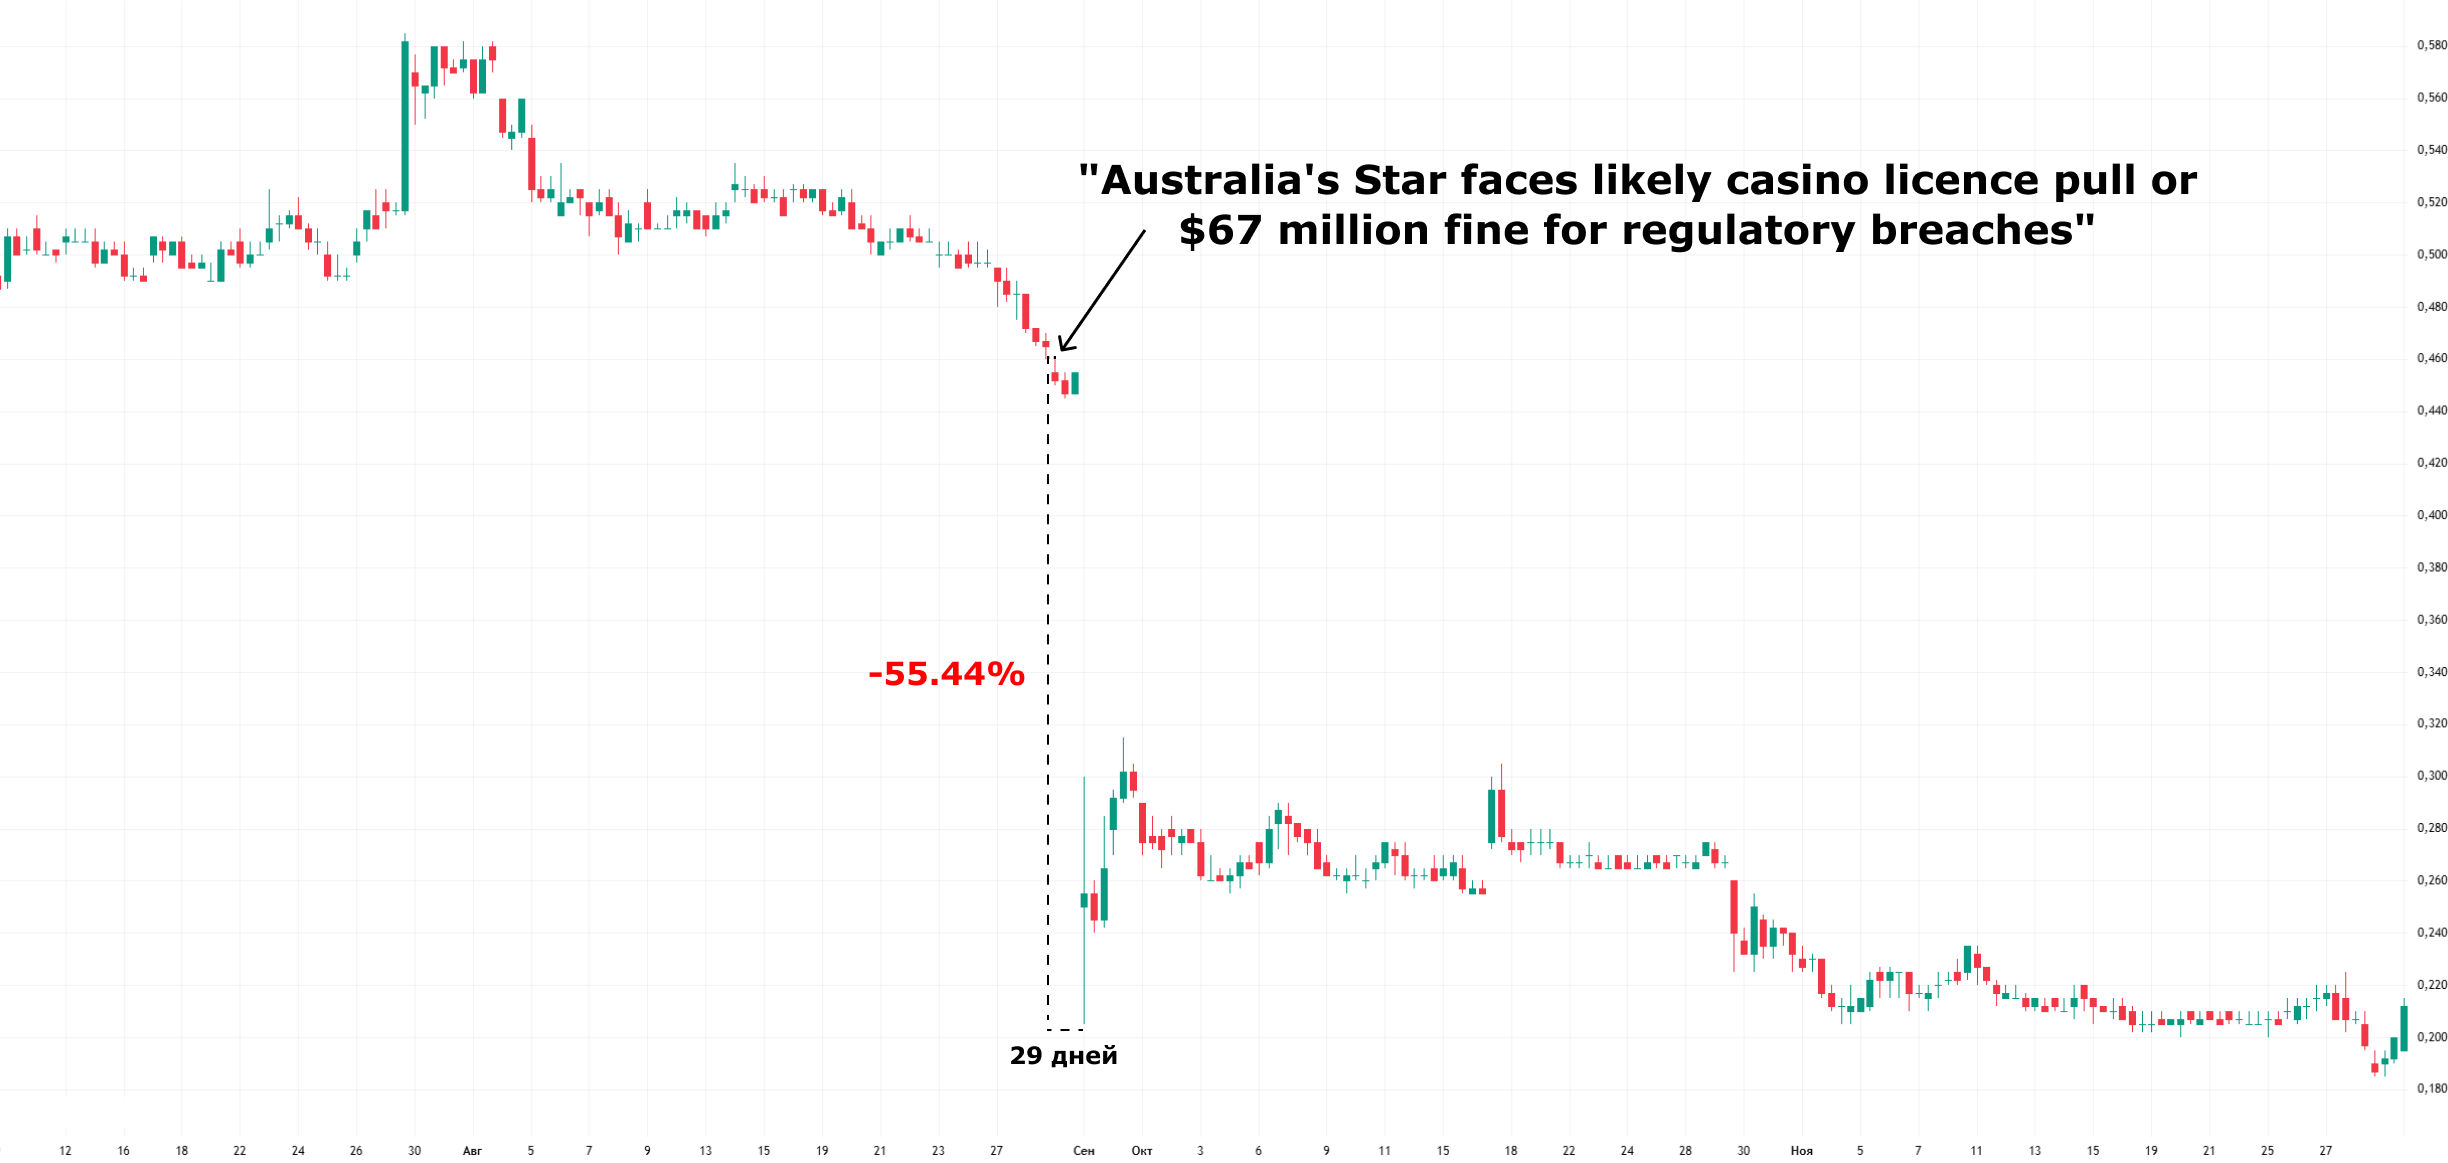
\includegraphics[width=1\linewidth]{img/star_entertainment.png}
    \caption{Пример того, как акции австралийской компании Star Entertainment Group LTD (SGR.ASX)
    обвалились и торговля ими была временно приостановлена из-за судебного разбирательства по отмыванию денег.}
    \label{fig:star_entertainment}
\end{figure}

Важно отметить, что торговля была приостановлена через сутки после публикации новости, что хоть
и является достаточным интервалом для обнаружения сигнала о продаже. Однако для рядового не вовлеченного
во внутридневную торговлю инвестора, данный сигнал весьма вероятно был бы незаметен, что привело бы
к ужасающей ситуации, когда инвестор не может продать обесценившийся актив и вынужден держать очевидный
убыток неопределенно длительный срок.

В обоих случаях, имея систему FinABYSS финансовый аналитик или инвестор мог бы одним из первых узнать
о данных инцидентах и незамедлительно отреагировать на рыночные сигналы. Простейшим способом своевременно
узнавать о триггерах является модуль активо-ориентированного отслеживания, который позволяет задать фильтры
по конкретному тикеру, источнику и тематике, чтобы получать только таргетированные сигналы.

В перспективе, после полной реализации и обучения архитектуры, предложенной в \hyperref[sec:architecture]{Разделе 3.1}, станет возможным
настройка фильтрации новостей по их сентименту, а также настройка пользовательского порога для обнаружения
значимо позитивных или негативных новостей.

Таким образом, FinABYSS выводит финансовую аналитику на совершенно новый уровень: вместо бессистемного
мониторинга СМИ и статей он получает готовые к действию алерты, визуализацию и прогнозную поддержку.
Семантическая карта уже сегодня становится неотъемлемой частью рабочего процесса, а по мере расширения
модальностей и внедрения предиктивного механизма её ценность будет лишь расти.


It is important to note that trading was halted 24 hours after the news was published, which is a sufficient
interval for a sell signal to be detected. However, for the average investor not involved in intraday trading,
this signal would very likely have been undetectable, leading to the dire situation of an investor unable to sell
a depreciating asset and forced to hold an obvious loss indefinitely.

In both cases, with FinABYSS, a financial analyst or investor would be among the first to recognize these incidents
and react immediately to market signals. The simplest way to learn about triggers in a timely manner is the asset-based
tracking module, which allows you to set filters by specific ticker, source, and topic to receive only targeted signals.

Eventually, once the architecture proposed in \hyperref[sec:architecture]{Section 3.1} is fully implemented and trained, it will be possible
to customize the filtering of news by its sentiment, as well as setting a custom threshold to detect meaningfully
positive or negative news.

FinABYSS thus takes financial analytics to a whole new level: instead of haphazard monitoring of media and articles,
it gets ready-to-action alerts, visualization, and predictive support. The semantic map is already becoming an integral
part of the workflow, and its value will only grow with the expansion of modalities and the introduction of a predictive
mechanism.

\subsection{Semantic De-duplication Solution}
\subsubsection{Математическая постановка}
\label{sec:semantic_deduplication}
\sloppy  % Helps to alleviate overfull hbox warnings

В рамках исследования был разработан новый подход к дедубликации, основанный на анализе семантического
одержимого объектов. Хотя в настоящей работе сущностью выступает текст, метод легко обобщается на любые
объекты, допускающие векторное представление в семантическом пространстве.

Каждая статья представляется в виде последовательности эмбеддингов:

\begin{equation}
    x_i \subset \mathbb{R}^{t\times d}
\end{equation}

где $t$ --- число токенов, а $d$ --- размерность семантического векторного пространства.
Для последующего анализа вместо набора эмбеддингов используется их выпуклая оболочка,
обозначаемая как $\operatorname{CH}(x_i)$ или, сокращенно, $\operatorname{CH}_i$. В качестве
меры уникальности текста применяется объем этой оболочки, $\mathrm{vol}(\operatorname{CH}_i)$.

\textbf{Пересечение выпуклых оболочек}. При прямом вычитании пересечений между
$\operatorname{CH}_i$ и оболочками других текстов может возникнуть проблема
множественного учета. Чтобы устранить кратное вычитание, применяется метод
включений–исключений.

Обозначим множество всех статей, кроме $i$, как

\begin{equation}
    \mathbb{I} = \{1, \ldots, N\} \setminus \{i\}.
\end{equation}

Пересечение $\operatorname{CH}_i$ с оболочками статей, индексированных подмножествами $\mathbb{J} \subseteq \mathbb{I}$, задается выражением:

\begin{equation}
    \mathrm{vol}\Big(\operatorname{CH}_i \cap \bigcap_{j \in \mathbb{J}}\operatorname{CH}_j\Big).
\end{equation}

Тогда объем пересечения $\operatorname{CH}_i$ с объединением оболочек остальных статей вычисляется по формуле:

\begin{equation}\label{eq:inclusion-exclusion_substituting}
    \mathrm{vol}\left(\operatorname{CH}_i \cap \bigcup_{j \in \mathbb{I}}\operatorname{CH}_j\right)
    =
    \sum_{k=1}^{N-1} (-1)^{k-1} \sum_{\substack{\mathbb{J} \subseteq \mathbb{I} \\ |\mathbb{J}| = k}}
    \mathrm{vol}\left(\operatorname{CH}_i \cap \bigcap_{j \in \mathbb{J}}\operatorname{CH}_j\right).
\end{equation}

Уникальность статьи $i$ определяется как доля объема её выпуклой оболочки, не задействованная в пересечениях с оболочками других статей:

\begin{equation}
    \mu_i = \frac{\mathrm{vol}\Big( \operatorname{CH}_i \setminus \bigcup_{j \in \mathbb{I}} \operatorname{CH}_j\Big)}{\mathrm{vol}\Big( \operatorname{CH}_i\Big)}.
\end{equation}

Преобразуя это определение с учетом разбиения $\operatorname{CH}_i$ на область пересечения и её дополнения, получаем:

\begin{equation}
    \mu_i = 1 - \frac{\mathrm{vol}\left(\operatorname{CH}_i \cap \bigcup_{j \in \mathbb{I}}\operatorname{CH}_j\right)}{\mathrm{vol}\left(\operatorname{CH}_i\right)}.
\end{equation}

Подставляя выражение по принципу включений–исключений, окончательная Формула \ref{eq:inclusion-exclusion_substituting} имеет вид:

\begin{equation}\label{eq:uniqueness}
    \mu_i = 1 - \frac{1}{\mathrm{vol}\big(\operatorname{CH}_i\big)}
    \sum_{k=1}^{N-1} (-1)^{k-1} \sum_{\substack{\mathbb{J} \subseteq \mathbb{I} \\ |\mathbb{J}| = k}}
    \mathrm{vol}\Big(\operatorname{CH}_i \cap \bigcap_{j \in \mathbb{J}}\operatorname{CH}_j\Big).
\end{equation}

Значение $\mu_i \in [0, 1]$ характеризует уникальность текста: $\mu_i = 1$ означает отсутствие пересечений с другими текстами
(полная уникальность), а $\mu_i = 0$ указывает на то, что семантический объём текста полностью занят пересечениями с оболочками других текстов.

\subsubsection{Преимущества и недостатки}
Предлагаемый метод основан на теоретически обоснованном представлении текста: каждая
статья трактуется как выпуклая оболочка эмбеддингов токенов, что позволяет четко определить
семантическое содержимое объекта, применить принцип включения–исключения, унаследованный из
теории множеств, для корректного вычисления объёма пересечений, а также нормировать результат
так, чтобы итоговая мера уникальности находилась в интервале $[0,1]$.

У данного подхода помимо теоретической стройности есть целый ряд дополнительных преимуществ:
\begin{itemize}
    \item Применение эмбеддингов для каждого токена позволяет уловить тонкие различия
    в семантическом содержании, а агрегирование посредством выпуклой оболочки обеспечивает
    обобщённое представление о содержании текста. Это даёт возможность сравнивать тексты
    различной длины и тематики в едином векторном пространстве.
    \item Нормировка метрики, выраженной числом в интервале $[0,1]$, упрощает интерпретацию.
\end{itemize}

С другой стороны, у метода есть и ряд основательных недостатков:

\begin{itemize}
    \item Выпуклая оболочка в высокоразмерном пространстве (например, 768-мерном) может существенно «растянуться».
    Это приводит к неинформативности получаемых объёмов, а геометрия оболочек может не отражать сложные распределения эмбеддингов.
    \item Эмбеддинги имеют сложную, зачастую нелинейную структуру. Выпуклая оболочка, являясь минимально необходимым выпуклым множеством,
    может включать экстремальные точки, что приводит к переоценке занимаемого пространства и, как следствие, к искажению оценок.
    \item Из-за того, что эмбеддинги могут содержать случайные шумовые компоненты или артефакты, выпуклая оболочка может быть чувствительна к выбросам.
    Это приводит к тому, что небольшие неточности в эмбеддингах могут непропорционально увеличить объём выпуклой оболочки, и, соответственно, исказить оценку уникальности.
    \item Построение выпуклой оболочки и вычисление объёмов в высокоразмерном пространстве является ресурсозатратной задачей. Применение принципа включения–исключения для
    корректного вычисления пересечений между оболочками текстов усложняет расчёты, особенно при большом количестве документов.
\end{itemize}

Все перечисленные проблемы могут критичным образом сказаться на использования данного метода на практике, однако некоторых проблем можно избежать инженерным образом.

Проблему чувствительности к шуму (пункт 3) можно частично нивелировать использованием токена [CLS] в качестве
центроида выпуклой оболочки. Введение коэффициента $\delta$ для нормирования «вогнутости» оболочки в направлении
эмбеддинга [CLS] позволяет снижать влияние шумовых компонентов.

Проблему вычислительных затрат (пункт 4) можно решать различными способами:

\begin{itemize}
    \item Регулирование числа включающих–исключающих пар (гиперпараметр $N$ в суммировании)
    позволяет получить приближённую оценку уникальности с уменьшением вычислительной нагрузки.
    \item Применение алгоритмов, таких как UMAP, t-SNE, PCA и других, может привести исходное пространство
    к более низкой размерности, что значительно сократит затраты на вычисления. При этом необходимо учитывать возможную потерю точности.
    \item Аппроксимация объёма методом Монте–Карло позволяет получить оценку при уменьшении вычислительных ресурсов.
\end{itemize}

Метод представления семантической уникальности текста через выпуклые оболочки эмбеддингов обладает рядом
теоретических преимуществ (сильная нормировка, применимость принципа включения–исключения и единообразная
интерпретация результата). Однако практическое применение требует решения проблем, связанных с высокой размерностью,
нелинейностью распределения эмбеддингов и существенными вычислительными затратами. Дальнейшие исследования
могут быть направлены на разработку более устойчивых и эффективных методов оценки уникальности с учетом
указанных ограничений.


    \newpage
    \specialsection{Заключение}
    \label{sec:conclusion}
    Настоящая работа затрагивает одну из наиболее перспективных и в то же время сложных задач современной
финансовой аналитики --- интерпретируемое  прогнозирование стоимости активов с точки зрения теории
эффективного рынка на основе аспектно-ориентированного анализа новостного потока с применением
современных архитектур глубокого обучения. Стремительное развитие LLM, а также их применение в задачах
финансовой аналитики продемонстрировали существенный прогресс по сравнению с классическими подходами,
однако одновременно обозначили ряд нерешённых проблем, касающихся как архитектурных ограничений
моделей, так и дефицита специализированных данных и средств интерпретации результатов. В рамках
настоящего исследования была предпринята попытка интеграции нескольких современных парадигм (DAPT,
ABSA, DTM, гибридная кластеризация и др.) в единое аналитическое решение с учётом специфики финансового
домена и требований к прозрачности модели.

Ключевым результатом работы стало проектирование и реализация прикладной архитектуры, позволяющей
обрабатывать длинные финансовые тексты (до 8192 токенов) с учётом их семантической и аспектной структуры.
Для этого была задействована новейшая архитектура ModernBERT, обладающая рядом существенных преимуществ
по сравнению с предыдущими версиями FinBERT и BERT. Среди них — повышенное контекстное окно, ротационные
позиционные кодировки, чередующийся механизм внимания и оптимизации, ориентированные на работу с большими
документами. Это позволило обрабатывать не только заголовки или краткие выдержки, как в большинстве
предыдущих исследований, но и полные статьи, пресс-релизы, аналитические обзоры, а также трансформировать
семантику длинных текстов в векторные представления, пригодные для кластеризации и последующего анализа.

Одним из наиболее значимых вкладов данной работы является построение пайплайна тематического моделирования,
в котором аспекты рассматриваются как тематические кластеры, выделяемые в эмбеддинговом пространстве текстов
с применением методов понижения размерности (UMAP) и иерархической кластеризации на основе плотности
(HDBSCAN). Такой подход позволяет обойти необходимость ручного определения аспектов и заранее фиксированных
словарей, что особенно важно в условиях постоянно изменяющейся терминологии, лексики и повестки дня финансового
домена. В отличие от классического ABSA, в предложенном решении извлечение аспектов осуществляется на уровне
нескольколатентных тем, что делает систему адаптивной и способной масштабироваться на новые информационные потоки
без ручной разметки.

Разработанная система сочетает  взаимодополняющих компонентов: глубокую эмбеддинговую модель,
компонент тематической агрегации, кластеризацию текстов, метрики плотностной валидации и визуализатор
интерактивной семантической карты. Совместное использование этих компонентов обеспечивает не только высокую
эффективность, но и интерпретируемость, которая является важнейшим требованием в управленческой и финансовой
аналитике. Например, предложенный механизм генерации названий тем с использованием GPT-4o и ранжирования
терминов на основе c-TF-IDF и MMR, позволяет наглядно представить, за счёт каких ключевых слов формируется
та или иная тема, а также какие документы вносят в неё основной вклад.

В ходе исследования было выявлено и проанализировано несколько существенных ограничений, возникающих
в процессе построения подобной системы. В частности, отсутствие открытых специализированных корпусов
финансовых текстов привело к необходимости создания собственного корпуса новостей с Yahoo! Finance, объём
которого превысил 15 ГБ. Также был зафиксирован ряд технических и теоретических проблем: отсутствие
консенсуса по методологии семантической дедубликации, трудности с обработкой длинных документов (например,
отчётов 10-K), а также невозможность справедливого сравнения моделей с помощью существующих бенчмарков,
основанных на коротких текстах (например, FLUE). Для преодоления этих проблем были предложены авторские
решения, включая математическую формализацию дедубликации на основе семантического объёма.

Метрики оценки качества кластеризации и тематического моделирования в данной работе также рассматривались
скрупулёзно. Помимо стандартного коэффициента силуэта, был задействован индекс DBCV --- специализированная
метрика для оценки кластеров произвольной формы с учётом плотности. Результаты показали, что применение
DBCV позволяет корректно отразить качество кластеризации в задачах, где классические метрики (например,
индекс Дэвиса–Болдена, Калински–Харабаша или VIASCKDE ) дают искажённую картину.

Особое внимание в работе было уделено не только архитектурной, но и методологической строгости. Этапы
построения пайплайна были продуманы с учётом требований воспроизводимости и масштабируемости, а также
потенциальной интеграции с количественными моделями. Поскольку задача аспектного анализа --- это не только
инструмент понимания текстов, но и средство улучшения прогноза динамики стоимости активов, предлагаемое
решение нацелено на последующую интеграцию с количественными предикторами. Тем самым работа закладывает
основу для гибридных подходов к прогнозированию, где сочетаются качественные и количественные источники
информации. Настоящее исследование является своего рода мостом между новейшими открытиями в области глубокого
обучения и областью финансов.

Важным теоретическим вкладом является также обсуждение связи между тематическим моделированием и аспектным
анализом. В данной работе показано, что аспекты в финансовых текстах могут быть интерпретированы как латентные
темы, выделяемые с помощью кластеризации в эмбеддинговом пространстве. Это открывает путь к унификации двух
ранее разрозненных направлений анализа текста — тематического моделирования и аспектного анализа сентимента.
Такой подход особенно эффективен в условиях отсутствия размеченных данных и высокой изменчивости тематики
финансовых публикаций. С другой стороны, исследование предлагает новый подход, который позволяет посмотреть
на определение и саму идею тональности текстов под другим, непредвзятым углом.

Подводя итоги, можно сформулировать основные достижения работы:

\begin{enumerate}
    \item Реализована архитектура интерпретируемой системы аспектно-ориентированного анализа финансовых новостей
    на основе ModernBERT, UMAP и HDBSCAN.
    \item Реализован подход к автоматическому извлечению тем (аспектов) без использования словарей и ручной разметки,
    для обеспечения возможности последующего агрегированием сентимента на уровне тем.
    \item Проведена детальная предобработка и сбор специализированного корпуса финансовых новостей, с учётом
    особенностей текстов (длина, дублирование, источники). Корпус исчисляется 1 миллиардом токенов и качественно
    спроектирован, включая богатые метаданные, что позволяет использовать его в смежных исследованиях.
    \item Разработан и формализован математический подход к семантической дедубликации, учитывающий ограниченность
    текстуального сравнения и необходимость анализа семантической уникальности.
    \item Проанализированы архитектурные преимущества ModernBERT по сравнению с BERT и FinBERT,
    а также выявлены направления дальнейшего повышения интерпретируемости моделей.
    \item Разработана высокофункциональная система для аналитики в области семантики финансовых публикаций,
    которая функционирует в режиме реального времени.
\end{enumerate}

Несмотря на достигнутые результаты, работа оставляет открытыми ряд направлений для будущих исследований.
Во-первых, необходимо обучение спроектированной архитектуры, включая экспертов и предиктивную модель,
с интеграцией временных рядов и количественными признаками для построения полноценного гибридного предиктора.
Во-вторых, перспективно развитие мультиагентной архитектуры, где модели различного уровня (например,
специализированные под различные типы документов) взаимодействуют в рамках единого пайплайна, что является
открытым полем для разработки финансового ассистента для семантического анализа публикаций. В-третьих,
дальнейшее исследование методов динамического тематического моделирования может позволить более точно
и интерпретируемо отслеживать эволюцию аспектов во времени, что критически важно в условиях изменчивого
информационного поля.

В целом, представленная работа закладывает фундамент для системного подхода к финансовому прогнозированию
с использованием больших языковых моделей в контексте теории эффективного рынка. Комбинация инженерной
реализации, математического анализа и теоретического обоснования делает предложенное решение не только
практико-ориентированным, но и значимым с точки зрения научной новизны.

    \newrefcontext[sorting=ntvy]
    \printbibliography[env=gostbibliography, title=Источники литературы]
\end{document}